\documentclass{beamer}
\usepackage{bm}
\usepackage{booktabs}
\usetheme{afm}

\usepackage[T1]{fontenc}
\usepackage{lmodern}
\title{Interest Rate Derivatives}
\subtitle{Part 2}
\course{Advanced Financial Modelling}
\author{\href{mailto:matteo.sani@unisi.it}{Matteo Sani}}

\begin{document}
	\begin{frame}[plain]
		\maketitle
	\end{frame}

	\section{No Arbitrage Theory}
	\subsection{No Arbitrage Principle\ldots}

		{
		\setbeamercovered{transparent}
		\begin{frame}{Fundamental Theorem of Asset Pricing I}
			Harrison and Pliska proved and formalized the following results:
			\begin{itemize}
				\item<1-> \textbf{The market is free of arbitrage if (and only if) there exists an \textcolor{maincolor}{equivalent martingale measure} (EMM) (i.e. a risk neutral measure)}.
				\item<0> The market is \textcolor{maincolor}{complete} if and only if the martingale measure is unique.

				(Note that market completeness means that any contingent claim can be replicated by a portfolio, or in other words that every asset in every possible state of the world has a price.)
				\item<0> In a complete and arbitrage-free market the price of any derivative is uniquely given, either by the value of the associated replicating strategy, or by the expectation of the discounted payoff under the risk-neutral measure
			\end{itemize}
		\end{frame}
	}

	\begin{frame}{No Arbitrage}
		\begin{itemize}
			\item Arbitrage opportunities rarely exist in practice. If and when they do, gains are extremely small, are typically short-lived and difficult to spot. \textcolor{maincolor}{Arbitrage exclusion in the mathematical model is close enough to reality}.
			\item An \textcolor{maincolor}{equivalent martingale measure} $\mathbb{Q}$ is a probability measure on the space $\Omega$ such that
			\begin{enumerate}
				\item $\mathbb{Q}$ is equivalent to $\mathbb{P}$ (real world measure);
				\item for any asset $A$ and for each time $t$, $0\le t\le T$ there exists a (martingale) price $\pi_t$
				\begin{equation*}
					\pi_t = \expect{Q}[D(t,T)V_A|\mathcal{F}_t]
				\end{equation*}
				More on $D(t, T)$ later.
			\end{enumerate}
		\end{itemize}
		\begin{block}{Definition}
			A \textbf{(probability) measure} ($\mathbb{P}, \mathbb{Q}\ldots$) is a mapping which associates a probability to each element in the sample space. Two measures are \textbf{equivalent} if they agree "on what is possible". Note the word \emph{possible}: the two measures can have different probabilities for the same event, but must have the same \emph{null-set} $\{x\in {\mathbb{P}}\mid p (x)=0\}$.
		\end{block}
	\end{frame}

	\begin{frame}{Martingales}
	\begin{itemize}
		\item In finance, a martingale is a process where the best guess for the future value (given all information today) is simply the current value.
		\item If the discounted price process $D_t S_t$ is a $\mathbb{Q}$-martingale, it guarantees that:
		\begin{enumerate}
			\item if the process weren't a martingale, there would be a systematic "drift" after accounting for the risk-free rate, implying a riskless profit by either borrowing to buy the asset or shorting it. The existence of $\mathbb{Q}$ ensures the market is mathematically "fair."
			\item without the martingale property, this simple expectation wouldn't work because you'd have to adjust for the "riskiness" of the payoff, which varies from person to person.
		\end{enumerate}
	\end{itemize}
	\end{frame}

	\subsection{Risk Neutral Measure}
	\begin{frame}{Risk Neutral Measure}
		\begin{itemize}
			\item The fundamental distinction between the \textbf{Physical Measure} ($\mathbb{P}$) and the \textbf{Risk-Neutral Measure} ($\mathbb{Q}$) lies in the \textcolor{maincolor}{drift of the underlying process}.

			\item \textbf{Physical Measure ($\mathbb{P}$):} reflects historical data and subjective expectations. The expected return of a risky asset includes a \textbf{risk premium} ($\mu = r + \text{risk premium}$), which is notoriously difficult to estimate.

			\item \textbf{Risk-Neutral Measure ($\mathbb{Q}$):} a mathematical construct (EMM) where all assets have an expected return equal to the \textcolor{maincolor}{risk-free rate} ($r$).

			\item It allows us to price derivatives using observable market data (like implied volatility) rather than unobservable risk preferences.

			\item Under the \textit{No-Arbitrage} assumption, $\mathbb{Q}$ is an \textit{implied distribution} extracted from liquid market instruments, used to ensure that the discounted price process is a \textcolor{maincolor}{$\mathbb{Q}$-martingale}.
		\end{itemize}
	\end{frame}

%		The Bottom Line: We don't use Q to predict where the stock will go. We use Q to ensure that our price for a complex derivative is consistent with the prices of simple derivatives already trading in the market.
%

	\begin{frame}{Breeden-Litzenberger Formula}
	\begin{itemize}
		\item Breeden and Litzenberger showed that with \emph{a continuous range of European call options} with different strikes ($K$), you can "tease out" the market's implied probability density function ($f_Q$).
		\begin{equation*}
		C(K,T)=e^{-rT}\int_K^{\infty}(S_T-K)f_Q(S_T)dS_T
		\end{equation*}
		\item Differentiate the call price $C$ with respect to $K$ (differentiating under the integral sign)
		\begin{equation*}
		\frac{\partial C}{\partial K}=e^{-rT}\frac{\partial}{\partial K} \int_K^{\infty}(S_T-K)f_Q(S_T)dS_T = \ldots = - e^{-rT}\int_K^{\infty}f(S_T)dS_T\,\,\text{(CDF } P(S_T > K))
		\end{equation*}
		\item By the Fundamental Theorem of Calculus
		\begin{equation}
			\frac{\partial^2 C}{\partial K^2}=-e^{-rT}\frac{\partial}{\partial K}\int_K^{\infty}f(S_T)dS_T = -e^{-rT}[-f(K)] \implies f(K)=e^{rT}\frac{\partial^2 C}{\partial K^2}
		\end{equation}
		\item The result tells us that the state-price density is proportional to the curvature of the call option price with respect to the strike.
	\end{itemize}
	\end{frame}

	\begin{frame}{Underlying PDF from Market Data}
		\begin{itemize}
			\item In the real world, we don't have a continuous line of strikes; we have discrete points. To find that second derivative, traders use a strategy called a \emph{Butterfly Spread}.
			\item A butterfly spread involves buying a call at strike $K-\Delta K$, selling two calls at strike $K$, and buying one call at $K+\Delta K$.
			\item The cost of this butterfly spread is essentially the market's "price" for the stock ending up exactly at strike $K$.
			\item If the market thinks a certain price is more likely under $\mathbb{Q}$, the butterfly at that strike will be more expensive.
		\end{itemize}
	\end{frame}

	\begin{frame}{Numerical Approach \colablink{https://colab.research.google.com/drive/1lEN6WOi-P4aj4kdb32W9SAcY4E24NQAT}}
		Take call option prices with the same maturity but different strikes on S\&P 500 (other parameters are $T=1.6329$, $r=0.009779$, $S=\$1036.2$).
		\begin{enumerate}
			\item With the option prices as a function of the strike, compute $\cfrac{d^2C}{dK^2}$ which should proxy the underlying PDF.
			\item Interpolate (with cubic-spline) the option prices, \emph{increasing} the number of points of the PDF;
			\item Remove strikes leading to negative density (brute force approach...surely there are better ways to deal with that).
		\end{enumerate}
	\end{frame}

	\begin{frame}{Numerical Approach (Results)}
		\begin{center}
			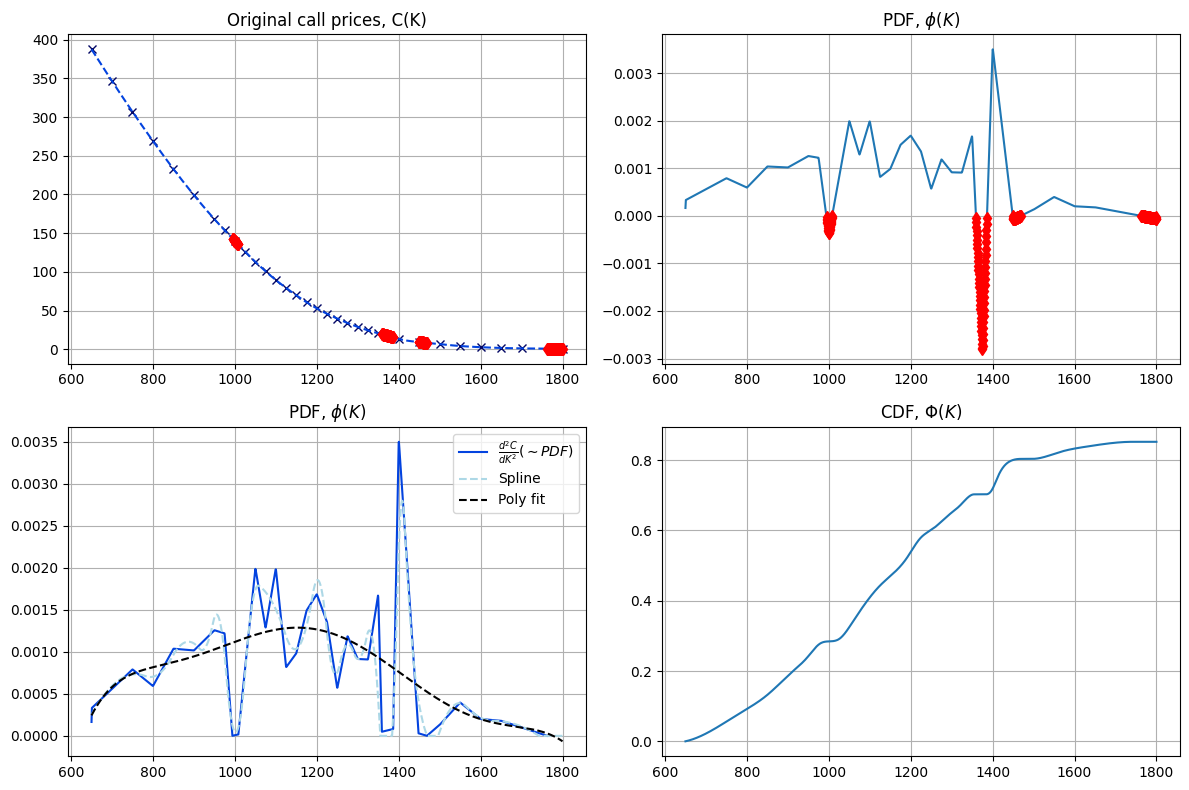
\includegraphics[width=0.75\linewidth]{images/Q_pdf_1}
		\end{center}
	\end{frame}

%		3. Extracting the "True" Q
%
%		When we apply this to market data, we see why the "Volatility Smile" matters.
%
%		In Black-Scholes the extracted $\mathbb{Q}$ distribution would be a perfect log-normal curve.
%
%		Because OTM Puts and Call are often "expensive" (high implied vol), the extracted $\mathbb{Q}$ distribution usually shows:
%		A fatter left tail, meaning the market assigns a higher risk-neutral probability to a market crash than a normal distribution would suggest.
%		"Fat tails" on both sides, suggesting "Black Swan" events are more likely than the math of the 1970s assumed.

	\begin{frame}{Numerical Approach (Vol Parametrization)}
		\begin{enumerate}
			\item Determine the implied volatilities from the option prices;
			\item fit the volatility surface (or a slice like in this case) with the preferred model (SVI);
			\begin{itemize}
				\item the name "Stochastic Volatility Inspired" comes from the fact that the model represents the asymptotic behavior of the Heston model;
				\item while Heston describes how volatility moves over time, SVI fits the volatility smile for a specific option expiration date.
				\begin{equation*}
					w(k) = a+b[\rho(k-m)+\sqrt{(k-m)^2+\sigma^2}]
				\end{equation*}
			\end{itemize}
			\item go back to the prices implied by the volatility fit;
			\item compute the second derivative of the obtained price distribution.
		\end{enumerate}
	\end{frame}


	\begin{frame}{Numerical Approach (SVI Model Results)}
	\begin{center}
		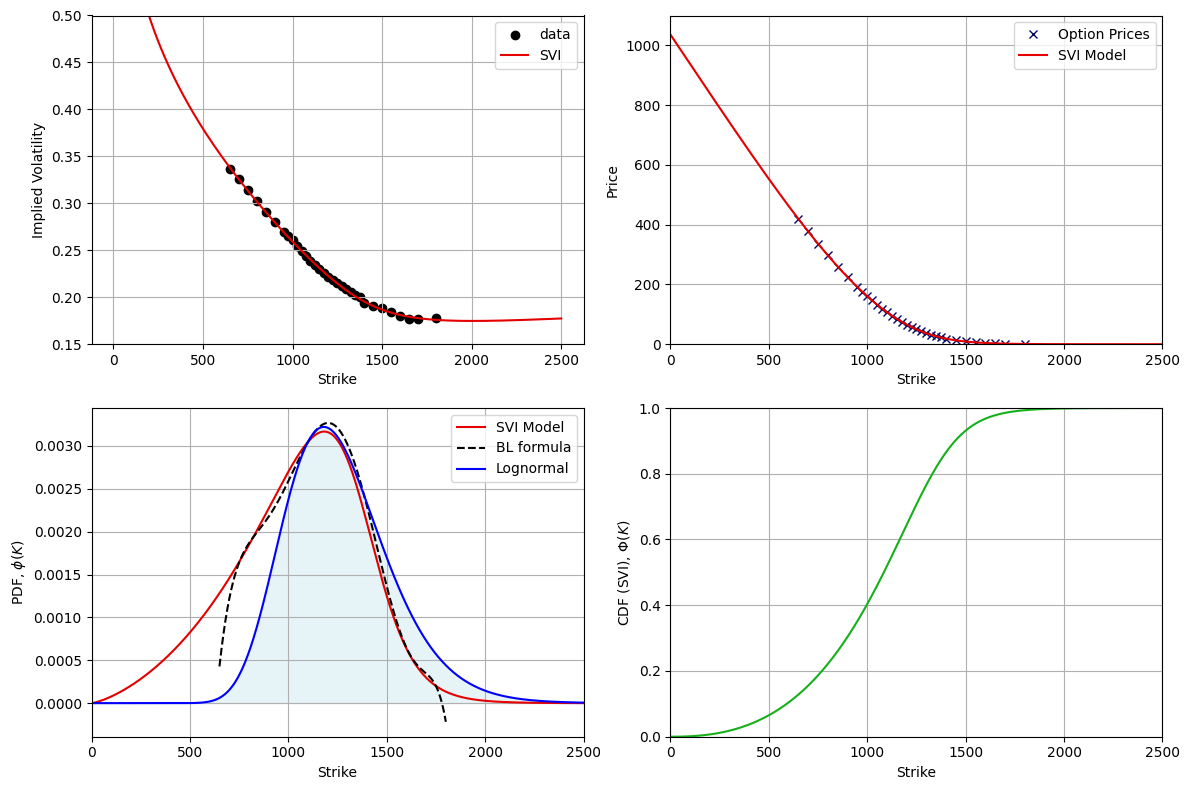
\includegraphics[width=0.75\linewidth]{images/Q_pdf_2}
	\end{center}
	\end{frame}


%		\begin{itemize}
%			\item  The difference between real world and risk neutral measures is in the treatment of the market price of risk.
%			\item If you tried to estimate the anticipated value of a stock based on how likely it is to go up or down, considering unique factors or market conditions that influence that specific asset, you would be including risk into the equation and, thus, would be looking at \textcolor{red}{real or physical probability}.
%			\item The \textcolor{red}{risk neutral measure}, instead, allows determination of a market-consistent value without making any assumption about the market price of risk. That is useful because the price of risk is not directly observable, but the market prices used to calibrate a risk-neutral generator are.
%			\item The risk neutral measure is a direct consequence of no arbitrage assumption. It is an \emph{implied probability distribution} from observable prices of tradable instruments, and used to determine \textcolor{red}{objective fair prices} for a financial instrument.
%		\end{itemize}
%	\end{frame}

	{
		\setbeamercovered{transparent}
	\begin{frame}{Fundamental Theorem of Asset Pricing II}
		Harrison and Pliska proved and formalized the following results:
		\begin{itemize}
			\item<0> The market is free of arbitrage if (and only if) there exists an \textcolor{maincolor}{equivalent martingale measure} (EMM) (i.e. a risk neutral measure).
			\item<1-> \textbf{The market is \textcolor{maincolor}{complete} if and only if the martingale measure is unique.}

			(Note that market completeness means that any contingent claim can be replicated by a portfolio, or in other words that every asset in every possible state of the world has a price.)
			\item<0> In a complete and arbitrage-free market the price of any derivative is uniquely given, either by the value of the associated replicating strategy, or by the expectation of the discounted payoff under the risk-neutral measure
			\begin{equation}
				\Pi_t = \expect{Q}[D(t,T)V_A|\mathcal{F}_t]
				\label{eq:risk_neutral_pricing}
			\end{equation}
		\end{itemize}
	\end{frame}
	}

	\begin{frame}{Market Completeness}
		\begin{itemize}
%		\item In a complete market any derivative payoff you can dream of can be perfectly "replicated" using a combination of the underlying stock and a bank account.
		\item  If you can build a synthetic version of a call option using $\Delta$ shares of stock and some cash, the price of the option must equal the cost of that synthetic portfolio.
		\item If there is only one way to replicate the payoff, there can only be one fair price. This "one fair price" corresponds to a unique Risk-Neutral Measure ($\mathbb{Q}$).
		\item In other words if you can perfectly \emph{hedge} an asset, your personal risk preference doesn't matter.
		\item  Whether you are a thrill-seeker or terrified of risk, the price is the same because the risk can be "traded away." In this case, Risk Neutrality is a mathematical result, not an assumption about human behavior.
	\end{itemize}
	\begin{block}{Definition}
		A \textbf{contingent claim} is a contract whose future payoff depends on the value of another “underlying” asset, or more generally, that is dependent on the realization of some uncertain future event $(S, X\ldots)$
	\end{block}
	\end{frame}

%Think of the Risk-Neutral Measure as a set of "shadow prices" for every possible future state of the world.
%
%In a Complete Market: Every future state is "reachable" by trading the available assets. Because you can trade into any state, the market "prices" every state perfectly. There is no room for ambiguity; hence, only one Q exists.
%
%In an Incomplete Market: There are "hidden" risks you cannot trade or hedge (e.g., sudden jumps in price, or volatility changing unexpectedly). Because you can't hedge these risks, there are multiple "valid" ways to price them depending on how much you dislike risk. This results in infinitely many valid Q measures.
%
%3. The Practical Consequences
%
%The difference between a unique measure and multiple measures is the difference between a single price and a price range.
%Market Status	Martingale Measure (Q)	Hedging Ability	Pricing
%Complete	Unique	Perfect replication (Delta hedging works)	A single "Fair Price"
%Incomplete	Infinitely Many	Residual risk remains (You can't hedge perfectly)	A "Bid-Ask" spread of theoretical prices
%4. Real-World Reality Check
%
%Is the real market complete? No.
%
%In the Black-Scholes model, the market is complete because we assume volatility is constant and there are no jumps. In that world, Q is unique.
%
%In the real world:
%
%Vol is stochastic: You can't perfectly hedge an option just by trading the stock; you'd also need to trade other options to hedge the "volatility risk" (Vega).
%
%Jumps happen: If a stock gaps down 20% overnight, you couldn't have traded "during" the jump to stay hedged.
%
%Because the real market is incomplete, we don't have a unique Q handed to us by God. Instead, we choose a Q by calibrating our models to the prices we see on our screens (the "Calibration Loop" we discussed earlier).
%Summary
%
%The theorem says: No gaps in hedging = No ambiguity in probability. If you can hedge everything, the math forces a single, unique probability distribution (Q) upon you. If you can't hedge everything, the "fair price" becomes a matter of opinion (or risk appetite), and many different Q measures could technically be "correct."
%
%
%1. The Connection: Uniqueness and Risk Neutrality
%
%The core "trick" of risk-neutral pricing is that if you can perfectly hedge an asset, your personal risk preference doesn't matter. * In a Complete Market (Unique Q): Because you can perfectly replicate a payoff using the underlying stock and cash, the "fair price" is simply the cost of that replication. Whether you are a thrill-seeker or terrified of risk, the price is the same because the risk can be "traded away." In this case, Risk Neutrality is a mathematical result, not an assumption about human behavior.
%
%In an Incomplete Market (Multiple $\mathbb{Q}$s): If you cannot perfectly hedge (e.g., because of sudden price jumps or changing volatility), you are left with "residual risk." To price that risk, you suddenly need to know how much someone is willing to pay to avoid it.
%
%Different "Risk-Neutral" measures Q1​,Q2​,... represent different levels of market-wide risk aversion.
%
%The "Uniqueness" disappears because the price now depends on the "Price of Risk."
%
%2. Why Incompleteness creates the "Volatility Smile"
%
%If the market were complete (as in the original Black-Scholes model), there would be only one Q—a perfect log-normal distribution. There would be no "Smile."
%
%The Volatility Smile exists precisely because the market is incomplete. Here is the chain of logic:
%
%Unhedgeable Risks: In the real world, stocks can "jump" (Gap risk) and volatility can "spike" (Vega risk). You cannot perfectly offset these with just the underlying stock.
%
%Risk Aversion: Because traders cannot perfectly hedge these "Black Swan" events, they demand a higher premium to take on that risk.
%
%The Smile as a "Risk Map": Traders bid up the price of Out-of-the-Money (OTM) puts to protect against crashes. When we "back-solve" these higher prices into the Black-Scholes formula, the volatility (σ) looks higher for those strikes.
%
%The Resulting Q: The "Implied" Q measure we extract from the smile is not a bell curve; it is skewed and fat-tailed. It represents the "Unique" measure the market has settled on by aggregating everyone's collective fear.
%
%3. The "Market Price of Risk" (λ)
%
%In a complete market, there is a unique relationship between the real-world P and the risk-neutral Q, governed by the Market Price of Risk (λ).
%
%Under P, the stock grows at μ=r+λσ.
%Under Q, we "subtract" that risk premium so the growth is just r.
%
%If the market is incomplete, λ is no longer a single number. It becomes a complex function (or even a stochastic process). This is why quantitative researchers spend so much time on Stochastic Volatility Models (like the Heston Model)—they are trying to find a mathematically consistent way to pick the "best" Q out of the infinite possibilities.

	\begin{frame}{Risk Neutral Pricing Foundations}
		Harrison and Pliska proved and formalized the following results:
		\begin{itemize}
			\item The market is free of arbitrage if (and only if) there exists an \textcolor{maincolor}{equivalent martingale measure} (EMM) (i.e. a risk-neutral measure).
			\item The market is complete if and only if the martingale measure is unique;
			\item \textbf{In a complete and arbitrage-free market the price of any derivative is uniquely given, either by the value of the associated replicating strategy, or by the expectation of the discounted payoff under the risk-neutral measure}
			\begin{equation}
				\Pi_t = \expect{Q}[D(t,T)V_A|\mathcal{F}_t]
				\label{eq:risk_neutral_pricing}
			\end{equation}
		\end{itemize}
	\end{frame}

	\begin{homework}
		\begin{frame}{\textcolor{white}{Homework}}
			\begin{itemize}
				\item[white] A stock is currently priced at $S_0=100$. In one year, it can either go up to $S_u=120$ or down to $S_d=90$. The risk-free rate is $r=5\%$ (annual compounding).
				\begin{itemize}
					\item[white] Calculate the risk-neutral probabilities $q$ and $1-q$;
					\item[white] If the "real-world" probability of an up-move is $p=0.7$, calculate the risk premium ($\mu - r$) that investors are demanding in the real world.
				\end{itemize}
				\item[white] Imagine you have to price a \emph{digital option} (a binary bet that pays \$1 if $S_T > K$), what can you do if you know PDF$_\mathbb{Q}$ ?
				\item[white] Suppose you are in a market with one underlying stock and two different risk-neutral measures, $\mathbb{Q}^1$ and $\mathbb{Q}^2$, both of which exclude arbitrage.
				\begin{itemize}
					\item[white] Is the market complete? Why or why not?
					\item[white] What does this imply for the pricing of a European Call option on that stock?
					\item[white] How does this relate to the Harrison-Pliska results in your slides?
				\end{itemize}
				\item[white] Consider the process $Y(t) = 2^{W(t)}$, where $\{W(T):t\geq 0\}$ is a standard Brownian motion. Is this a martingale ?
%				\item[white]  Show that the exponential SDE
%				\begin{equation*}
%					dX_t = A_t X_tdW_t,\quad X_0=x_0
%				\end{equation*}
%				has the following solution
%				\begin{equation*}
%					X_t = x_0 e^{-\frac{1}{2}\int_0^t A_0^2 ds+\int_0^t A_s dB_s}
%				\end{equation*}
			\end{itemize}
		\end{frame}
	\end{homework}


	\begin{frame}{Single Curve Approach}
		\begin{block}{Disclaimer}
			What follows is a detailed exposition of the classic \textcolor{maincolor}{single curve} approach mainly for interest rate derivatives.

			Today a \textcolor{maincolor}{multi-curve approach} is
			used in practical applications; nevertheless you need to understand
			deeply this basic approach as a prerequisite for the extension to the
			multi-curve model.
		\end{block}
	\end{frame}

\subsection{Money Market Account}
\begin{frame}{Money Market Account}
	\begin{itemize}
		\item<0-> The \textcolor{maincolor}{money market account} represents a risk-less investment, where profit is accrued continuously at the risk-free rate, and its value is denoted by $B(t)$.
		\item<1-> We assume $B(0)=1$ and by definition
		\begin{equation}
			dB(t) = r(t)B(t)dt
		\end{equation}
		\item<2-> This SDE can be solved through variable separation
		\begin{equation}
			\begin{gathered}
				\frac{dB_t}{B_t} = r_t dt \implies \int_0^t \frac{dB_t}{B_t} = \int_0^t r_s ds \\
				\implies \log\frac{B_t}{B_0} = \int_0^t r_s ds \implies \boxed{B(t) = \exp\left(\int_0^t r_s ds\right)}
			\end{gathered}
		\end{equation}
		where $r_t$ is referred to as \textcolor{maincolor}{instantaneous spot rate} or \textcolor{maincolor}{short rate}.
	\end{itemize}
\end{frame}

\begin{frame}{Money Market Account}
	\begin{itemize}
		\item<0-> The \emph{short rate} $r_t$ can be modeled either by a deterministic or a stochastic process.
		\item<1-> \textbf{Deterministic case}: from the definition of money market account, if I have $A$ units of currency at time 0, it follows that
		\begin{equation*}
			V(0) = A\cdot B(0) \implies V(t) = A\cdot B(t)
		\end{equation*}
		\item<2-> If we want to have at time $T$ exactly 1 unit of currency
		\begin{equation*}
			A\cdot B(T) = 1 \implies A = \frac{1}{B(T)} \implies AB(t) = \frac{B(t)}{B(T)}
		\end{equation*}
		hence $\frac{B(t)}{B(T)}$ is \textcolor{maincolor}{the value of one unit of currency payable at time $T$ seen from $t$}.
			\end{itemize}
\end{frame}

\subsection{Stochastic Discount Factor and Zero Coupon Bond}
\begin{frame}{Stochastic Discount Factor}
	\uncover<1->{
		\begin{block}{Definition}
			The \textcolor{maincolor}{(stochastic) discount factor} $D(t, T)$ is the amount at time $t$ that is \emph{equivalent} to one unit of currency payable at time $T$ and is given by
			\begin{equation}
				D(t, T) = \frac{B(t)}{B(T)} = e^{-\int_t^T r_s ds}
			\end{equation}
	\end{block}}
	\begin{itemize}
		\item<2-> Can you guess what is the unit of measurement of a discount factor ?
		\item<3-> In many pricing application (e.g. Black-Scholes formula) $r$ is assumed to be a \textcolor{maincolor}{deterministic} function of time, and so are $B(t)$ and $D(t,T)$:
		\begin{itemize}
			\item<3-> this is motivated by the small influence interest rate variations have on equity prices.
		\end{itemize}
		\item<4-> When dealing with interest rate products, $r$ becomes the main actor, so the deterministic assumption must be dropped.
	\end{itemize}
\end{frame}

\begin{frame}{Deterministic vs Stochastic}
	\begin{itemize}
		\item<0-> Recall the risk-neutral pricing formula
		\begin{equation*}
			\Pi_t = \expect{Q^B}[D(t,T)A|\mathcal{F}_t]
		\end{equation*}
		(the risk-neutral measure is often denoted by $\mathbb{Q}^0$, $\mathbb{Q}^B$ or simply $\mathbb{Q}$, and similarly for the expectations).
		\item<1-> When \textcolor{maincolor}{interest rates are deterministic}, the exponential can be brought out of the expectation
		\begin{equation*}
			\Pi_t = e^{-\int_t^T r_s ds} \expect{Q}\left[A|\mathcal{F}_t\right]
		\end{equation*}
		\item<2-> If in addition \textcolor{maincolor}{rates are constant} (e.g. Black-Scholes or Heston models)
		\begin{equation*}
			\Pi_t = e^{-r(T-t)}\expect{Q}\left[A|\mathcal{F}_t\right]
		\end{equation*}
	\end{itemize}
\end{frame}

\begin{frame}{Why the Money Market Account is "Special"}
	\begin{itemize}
		\item A fundamental requirement of the Asset Pricing Theorems is that the \textbf{discounted price process} must be a martingale. %(since a stock that grows on average cannot be martingale; it must be "leveled out" by the risk-free rate).
		\item You might wonder: why use $B_t$ ? Why not discount by the price of gold or another stock ?
		\item The money market account is the only asset with \textbf{locally}$^{*}$ zero variance. It grows predictably at rate $r$. %(Choosing $B_t$ as a \emph{numeraire} defines the Risk-Neutral Measure, whereas choosing $P(t,T)$ as a numeraire would define the Forward Measure.)
		\item When we change the measure from $\mathbb{P}$ to $\mathbb{Q}$, we are specifically looking for the probability set that makes the expected return of any asset equal to the return of $B_t$.
	\end{itemize}
	\vfill
	\begin{tcolorbox}[colback=gray!5, colframe=maincolor, arc=0mm, boxrule=0.5pt]
		\footnotesize
		 $^{*}$ At time $t$, $r_t$ is known ($\mathcal{F}_t$-measurable). In $[t, t+dt]$, $B_t$ is determined only by the drift $r_t B_t dt$, no "shock" from a Brownian motion. Over $[t,T]$, $B_T=\exp{\int_t^T r_s ds}$ is random because we don't know the future path of $r_s$.
	\end{tcolorbox}
\end{frame}

%This is a crucial technical point. In advanced stochastic calculus for finance, we distinguish between assets that are stochastic (risky) and those that are locally deterministic.
%
%When we say the Money Market Account ($B_t$) has locally zero variance, we are making a statement about its diffusion term (the $dW_t$ component) in a stochastic differential equation (SDE).
%
%Let’s look at the SDEs for a risky stock ($S_t$) and the money market account ($B_t$):
%
%For the Stock ($S_t$):
%
%$dS_t=\mu S_t dt+\sigma S_t dW_t$
%
%Variance over dt: The variance of the change $dS_t$ is $\sigma^2 S_t^2 dt$. This is non-zero as long as $\sigma >0$.
%
%For the Money Market Account:
%$dB_t =r_t B_t dt + 0\cdot dW_t


%Summary: B_t is locally riskless but globally risky (if rates are stochastic).
%
%3. Why this matters for the EMM
%
%This unique property is why we use B_t to define the "Risk-Neutral" world.
%
%If you tried to use a stock as a numeraire, the "baseline" you are measuring against would itself be jumping around due to its own diffusion term. Because B_t has no diffusion, it acts as a "clean" filter. When we divide a risky asset S_t by B_t, we aren't adding any new sources of noise; we are simply "peeling away" the predictable growth ($r$) to see if the remaining process is a martingale.


\begin{frame}{Zero Coupon Bond}
	\begin{itemize}
		\item<1-> \textcolor{maincolor}{Zero Coupon Bond} (ZCB) is a contract that pays one unit of money at time $T$. Its price at time $t$ is denoted by $P(t,T)$, and by definition $P(T,T) = 1$.
		\item<1-> What is the relation between $P(t,T)$ and $D(t,T)$ ? \\
	\end{itemize}
	\uncover<2->{
		\begin{table}[bt]
			\centering
			\footnotesize % Professional sizing for slides
			\renewcommand{\arraystretch}{1.4}
			\begin{tabular}{|l|c|c|}
				\hline
				\textbf{Property} & \textbf{Discount Factor $D(t,T)$} & \textbf{ZC Bond $P(t,T)$} \\ \hline
				\textbf{Nature} & Amount equivalent to \$1 & Price of a tradable contract \\ \hline
				\textbf{Deterministic} & \multicolumn{2}{c|}{$D(t,T) = P(t,T) = e^{-\int_t^T r_s ds}$} \\ \hline
				\textbf{Stochastic} & \textcolor{maincolor}{Random} ($\mathcal{F}_T$-measurable) & \textcolor{maincolor}{Known} ($\mathcal{F}_t$-measurable) \\ \hline
				\textbf{Relationship} & --- & $P(t, T) = \mathbb{E}^{\mathbb{Q}}[D(t, T)|\mathcal{F}_t]$ \\ \hline
			\end{tabular}
		\end{table}}
\end{frame}

\begin{frame}{Spot Interest Rate}
	\begin{itemize}
		\item  If you invest 1 unit of currency at time $t$ for a duration of $\tau = T-t$, and the annual simple interest rate is $L$, the (simply compounded) value at maturity $T$ is:
		\begin{equation*}
		V(T)=1+(L\cdot \tau)
		\end{equation*}
		\item A Zero-Coupon Bond $P(t,T)$ represents the price today ($t$) of 1 unit of currency to be received at maturity ($T$).
		\item If we invest $P(t,T)$ today, it must grow to exactly 1 at time $T$, so
		\begin{equation}
		P(t,T)\cdot (1+L\cdot\tau)=1 \implies L(t,T)=\frac{(1-P(t,T))}{\tau(t,T)P(t,T)}
		\end{equation}
		which represent the simply-compounded \textcolor{maincolor}{spot interest rate}
		\item The \textcolor{maincolor}{yield curve} at time $t$ is the graph of:
		\begin{equation*}
			T\rightarrowtail L(t, T)
		\end{equation*}
	\end{itemize}
\end{frame}

\begin{homework}
	\begin{frame}{\textcolor{white}{The Expectation Paradox}}
		\begin{itemize}
			\item[white] In a stochastic interest rate world, is it true that
			\begin{equation*}
				P(t,T)=\mathbb{E}^{\mathbb{Q}}\left[ \frac{1}{e^{\int_t^T r_s ds}} |\mathcal{F}_t \right] ?
			\end{equation*}
			\textbf{Hint}: use Jensen's inequality
		\end{itemize}
	\end{frame}
\end{homework}







\section{Forward Rate Agreement}
\begin{frame}{Forward Rate Agreement}
	\begin{itemize}
		\item<1-> A \textcolor{maincolor}{Forward Rate Agreement} (FRA) is a contract involving three time instants: %the current time $t$, the fixing time $T>t$, and the maturity time $S>T$.
		\begin{equation*}
			\underbrace{t}_{\text{current time}} \leq \underbrace{T}_{\text{fixing time}} \leq\underbrace{S}_{\text{maturity}}
		\end{equation*}
		\item<2-> The FRA payout consists of an exchange of interest rate flows calculated for the time period $\tau=S-T$. At the maturity $S$, a fixed payment based on a fixed rate $K$ is exchanged against a floating payment based on the spot rate $L(T, S)$ whose value is known only in $T$.
		\item<3-> This contract allows to lock-in the interest rate between times $T$ and $S$ at a desired value $K$.

%		\noindent
%		(\textbf{note:} interest rate flows are calculated using the simple compounding law).
	\end{itemize}
\end{frame}

\begin{frame}{FRA Example}
	\begin{itemize}
		\item A FRA is an agreement that enables to \emph{hedge} against unfavourable movements in interest rates by fixing a rate on a notional amount that is (usually) of the same size and term as the exposure that starts sometime in the future.
		\vfill
		\begin{center}
			\includegraphics[width=0.9\linewidth]{images/FRA_diagram}
		\end{center}
	\end{itemize}
\end{frame}

\begin{frame}{FRA Time Table}
	\begin{itemize}
		\item Consider a $1\times 3$ FRA (1-month into 3-month): the 1 in the $1\times 3$ refers to 1 month' time when settlement (fixing) takes place, and the 3 to the expiry date of the FRA from deal date.
		%, i.e. the rate quoted for the FRA is a 1-month rate at the time of settlement
		\begin{center}
			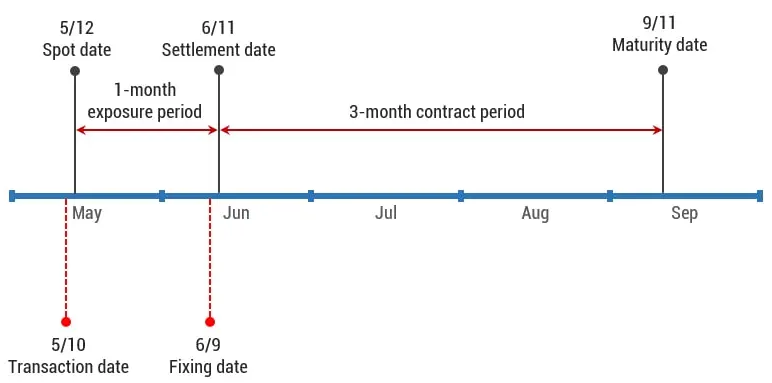
\includegraphics[width=0.8\linewidth]{images/fra_timeline}
		\end{center}
	\end{itemize}
\end{frame}

\begin{frame}{FRA: Formalization of the Contract}
	\begin{itemize}
		\item<1-> Formally, at time $S$ one receives $N\cdot\tau(T, S)\cdot K$ units of currency and pays the amount $N\cdot\tau(T,S)\cdot L(T,S)$, where $N$ is the contract nominal value.
		\item<2-> Thus, at time $S$, the future (and \textbf{today unknown}) payout of the contract is:
		\begin{equation}
			N\cdot\tau(T,S)\cdot(K-L(T,S))
			\label{eq:fra_payoff}
		\end{equation}
		\item<3-> In order to assign a \textbf{value} at this contract we have to tackle two issues:
		\begin{itemize}
			\item<3-> estimate the future value of $L(T, S)$;
			\item<3-> discount the result from $S$ to today (time $t$).
		\end{itemize}
		\item<4-> There are several ways to arrive at the final result: \textbf{no arbitrage is the common denominator.}
%
%		The "Law of One Price": Whether you value the FRA by:
%
%		Using the Expectation under a specific probability measure (Martingale approach).
%
%		Building a Replicating Portfolio (using existing bonds to mimic the FRA payoff).
%
%		Using the Forward Price formula.
%
%		...you must get the same price. If different methods gave different prices, an arbitrage opportunity would exist between the methods.
	\end{itemize}
\end{frame}

\begin{frame}{The Tower Property: "Information Nesting"}

	\begin{block}{Definition}
		Consider a filtered probability space: $(\Omega, \mathcal{F}_{t\geq 0}, \mathbb{P})$.
		For any $0\leq s \leq t$ and stochastic process $\{X_t\}_{t\geq 0}$, we have the following \emph{tower property}:
		\begin{equation}
		\mathbb{E}[\mathbb{E}[X|\mathcal{F}_t]|\mathcal{F}_s]=\mathbb{E}[X|\mathcal{F}_s]
		\end{equation}
		\textit{The best guess of a future best guess is just your current best guess.}
	\end{block}

	\begin{tcolorbox}[colback=gray!5, colframe=maincolor, arc=0mm, boxrule=0.5pt]
		\footnotesize
			Imagine you want to predict the price of a stock $X$ on \textbf{Friday}:
		\begin{itemize}
			\item $\mathcal{F}_s$ (Monday): You know today's price.
			\item $\mathcal{F}_t$ (Wednesday): You will know the mid-week earnings report.
		\end{itemize}
		\vspace{0.2cm}
		On \textbf{Monday}, if you try to guess what your \textbf{Wednesday} prediction will be, you can only rely on what you know \textbf{now}. The "extra" information arriving on Wednesday is currently unknown and averages to zero.

		\centering
		\textit{The "Tower" collapses because you cannot predict future news.}
	\end{tcolorbox}
\end{frame}

\subsection{FRA Valuation}
\begin{frame}{FRA Valuation: Brigo-Mercurio Approach}
	\begin{itemize}
		\only<1-1>{
			\item Substitute to $L(T,S)$ in \cref{eq:fra_payoff} its expression as a function of the zero-coupon bond price $P$, discount and take the expectation
			\begin{equation*}
				\mathbb{E}\Bigg[D(t, S) N\bigg(\tau K + 1 - \frac{1}{P(T, S)}\bigg)\bigg| \mathcal{F}_t\Bigg]
			\end{equation*}
			\item Under no-arbitrage, the "fair" future rate $L(T,S)$ isn't just a guess; it is mathematically locked to the prices of Zero-Coupon Bonds today. If the forward rate in the FRA were different from the rate you could create by buying and selling bonds of different maturities, a trader could exploit the difference for a guaranteed profit.
		}
		\only<2->{
			\item First interpret $A$ as an amount of money held at time $S$
			\begin{equation*}
				\mathbb{E}\Bigg[D(t, S) N\bigg(\tau K + 1 - \underbrace{\frac{1}{P(T, S)}}_{A}\bigg)\bigg| \mathcal{F}_t\Bigg]
			\end{equation*}
		}
		\item<2-> At time $T$ it's worth 1, indeed

		\begin{align*}
			\mathbb{E}_t\left[ D(T,S)\frac{1}{P(T,S)}\right]  = \mathbb{E}_t\left[D(t,T)\mathbb{E}_T\left[D(T,S)\frac{1}{P(T,S)}\right] \right] =\\
			= \mathbb{E}_t\left[D(t,T)P(T,S)\frac{1}{P(T,S)}\right] = \mathbb{E}_t[D(t,T)] = P(t,T)
		\end{align*}
		since $\mathbb{E}_T[D(T,S)]=P(T,S)$, and we discount it back to time $t$.
	\end{itemize}
\end{frame}

\begin{frame}{FRA Valuation: Brigo-Mercurio Approach}
	\begin{itemize}
		\item On the other hand $B$
		\begin{equation*}
			\mathbb{E}\Bigg[D(t, S) N\bigg(\underbrace{\tau K + 1}_{B} - \frac{1}{P(T, S)}\bigg)\bigg| \mathcal{F}_t\Bigg]
		\end{equation*}
		\item<1-> Since the payout is expressed at time $S$, at time $t$ it becomes:
		\begin{equation*}
			K\cdot\tau\cdot P(t,S) + P(t, S)
		\end{equation*}.
		\item<2-> Collecting the two terms we get
		\begin{equation}
			\boxed{\textbf{FRA}(t,T,S,\tau,N,K)=N[\underbrace{K\cdot\tau\cdot P(t,S)+P(t,S)}_{B}-\underbrace{P(t,T)}_{A}]}
			\label{eq:fra_valuation}
		\end{equation}
	\end{itemize}
	\only<2->\myendproof
\end{frame}

\begin{frame}{A Linear Derivative  \colablink{https://colab.research.google.com/drive/1jjryIuf_E0e51evaYGYpIkjq1ifi5kdt}}
	\begin{itemize}
		\item A Forward Rate Agreement (FRA) is classified as a linear derivative because its value at maturity changes in direct proportion to the change in the underlying interest rate.
		\item Unlike options, an FRA does not have a "kink" in its payoff profile. If the market interest rate moves up by 1 basis point, the value of the FRA moves by a fixed amount\ldots($\textbf{FRA}(L)=mL+c$).
		\item Understanding linearity is crucial for Portfolio Risk Management.
 		\begin{center}
		 	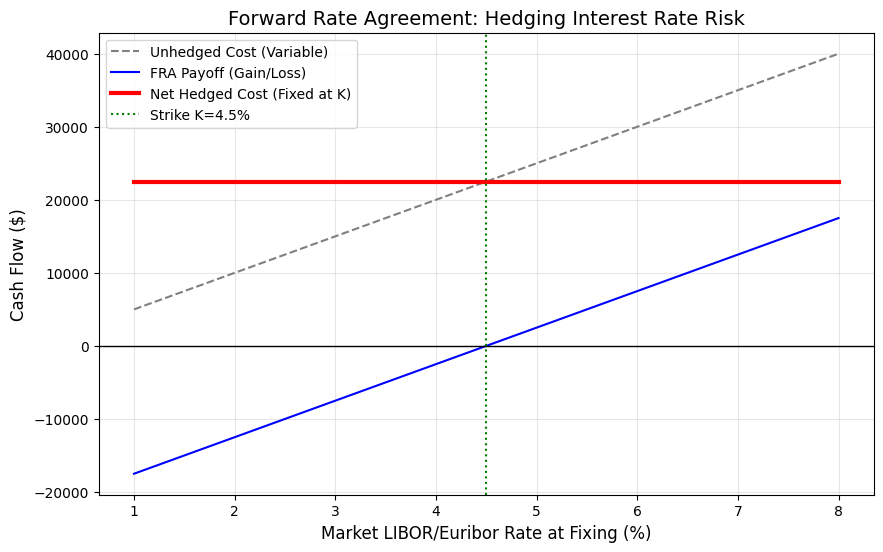
\includegraphics[width=0.5\linewidth]{images/FRA_linearity}
		 \end{center}
	\end{itemize}
\end{frame}

%\subsection{FRA Detailed Proof}
%\begin{frame}{FRA Detailed Proof}
%	\begin{itemize}
%		\item<1-> Let's start from the risk neutral pricing formula
%		\begin{equation} \textbf{FRA} =
%			\expectt{Q}{t}[\tau D(t,S)(K - L(T,S))] = 	\expectt{Q}{t}[\tau D(t,S)K - \tau D(t,S)L(T,S)]
%			\label{eq:fra_as_expectation}
%		\end{equation}
%		(\textbf{note:} to ease the notation $\expectt{Q}{t}[X] = \expect{Q}[X|\mathcal{F}_t]$).
%		\item<2-> From which we can easily derive using the definition of \textbf{ZCB} value
%		\begin{equation*}
%			\begin{aligned}
%				\textbf{FRA} = \tau &K\expectt{Q}{t}[D(t,S)] - \expectt{Q}{t}[\tau D(t,S)L(T,S)] = \\
%				&=\tau KP(t,S) - \expectt{Q}{t}[\tau D(t,S)L(T,S)]
%			\end{aligned}
%		\end{equation*}
%		\item<3-> For a discount factor the following holds
%		\begin{equation*}
%			D(t,S) = D(t,T)D(T,S)\quad(\text{since }e^{-\int_t^S r_s ds} = e^{-\int_t^T r_s ds - \int_T^S r_s ds})
%		\end{equation*}
%	\end{itemize}
%\end{frame}
%
%\begin{frame}{FRA Detailed Proof}
%	\begin{itemize}
%		\item<1-> So we get (omitting the risk-neutral symbol from the expectation)
%		\begin{equation*}
%			\textbf{FRA} = \tau KP(t,S)-\mathbb{E}_t[\tau D(t,T)D(T,S)L(T,S)]
%		\end{equation*}
%		\item<2-> Then using the tower expectation property
%		\begin{equation*}
%			\textbf{FRA} = \tau KP(t,S) - \mathbb{E}_t[\mathbb{E}_T[\tau D(t,T)D(T,S)L(T,S)]]
%		\end{equation*}
%		\item<3-> Last equation can be transformed as
%		\begin{equation*}
%			\textbf{FRA} = \tau KP(t,S) - \mathbb{E}_t[\tau D(t,T)L(T,S)\mathbb{E}_T[D(T,S)]]
%		\end{equation*}
%		\item<4-> From which
%		\begin{equation*}
%			\textbf{FRA} = \tau KP(t,S) - \expectt{Q}{t}[\tau D(t,T)L(T,S)P(T,S)]
%		\end{equation*}
%	\end{itemize}
%\end{frame}
%
%\begin{frame}{FRA Detailed Proof}
%	\begin{itemize}
%		\item<1-> Then using the definition of IBOR rate $L(t,T)=\frac{(1-P(t,T))}{\tau(t,T)P(t,T)}$
%		\begin{equation*}
%			\begin{aligned}
%				\textbf{FRA} &= \tau KP(t,S) - \mathbb{E}_t\left[\cancel{\tau}D(t,T)\left(\cfrac{1-P(T,S)}{\cancel{\tau} P(T,S)}\right)P(T,S)\right] = \\
%				&=\tau KP(t,S)-\mathbb{E}_t\left[D(t,T)P(T,S)\left(\frac{1}{P(T,S)}-1\right)\right]= \\
%				&=\tau KP(t,S)-\mathbb{E}_t[D(t,T)] + \mathbb{E}_t[D(t,T)P(T,S)]
%			\end{aligned}
%		\end{equation*}
%		\item<2-> The last term can be expressed in terms of $D$
%		\begin{equation*}
%			\textbf{FRA} = \tau KP(t,S)-\mathbb{E}_t[D(t,T)] + \mathbb{E}_t\left[D(t,T)\mathbb{E}_T[D(T,S)]\right]
%		\end{equation*}
%	\end{itemize}
%\end{frame}
%
%\begin{frame}{FRA Detailed Proof}
%	\begin{itemize}
%		\item<1-> Bringing the discount factor inside the expectation
%		\begin{equation*}
%			\begin{aligned}
%				\textbf{FRA} &= \tau KP(t,S)-\mathbb{E}_t[D(t,T)] + \mathbb{E}_t\left[D(t,T)\mathbb{E}_T[D(T,S)]\right] \\
%				&=\tau KP(t,S)-\mathbb{E}_t[D(t,T)] + \mathbb{E}_t\left[\mathbb{E}_T[D(t,T)D(T,S)]\right]=\\
%				&=\tau KP(t,S)-\mathbb{E}_t[D(t,T)] + \mathbb{E}_t\left[\mathbb{E}_T[D(t,S)]\right]
%			\end{aligned}
%		\end{equation*}
%		\item<2-> Then applying the law of iterated expectations we arrive at the final result
%		\begin{equation*}
%			\begin{aligned}
%				\textbf{FRA} &= \tau KP(t,S)-\expectt{Q}{t}[D(t,T)] + \expectt{Q}{t}[D(t,S)] = \\
%				&= \boxed{\tau KP(t,S) - P(t,T) + P(t,S)}
%			\end{aligned}
%		\end{equation*}
%		\myendproof
%	\end{itemize}
%	%\pause
%	%\begin{tikzpicture}[remember picture,overlay]
%	%	\node[xshift=6.cm,yshift=-4.cm] (image) at (current page.center) {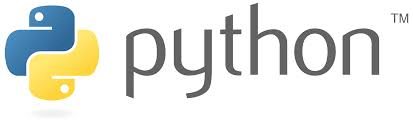
\includegraphics[width=80px]{python}};
%	%\end{tikzpicture}
%\end{frame}

\subsection{Forward Rate Definition}

\begin{frame}{The Simply-Compounded Forward Rate}
	\begin{block}{Definition}
		The \textcolor{maincolor}{Forward Libor Rate} $F(t; T, S)$ is the fixed rate $K$ that makes the value of a FRA equal to zero at time $t$.
		Setting $\textbf{FRA}(t, T, S, \tau, N, K) = 0$ in our previous result:
		\begin{equation*}
			F\cdot\tau\cdot P(t, S) + P(t, S) - P(t, T) = 0
		\end{equation*}
		and solving for $F$:
		\begin{equation}
			\boxed{F(t; T, S) = \frac{1}{\tau} \left( \frac{P(t, T)}{P(t, S)} - 1 \right)}
			\label{eq:forward_rate_definition}
		\end{equation}
		It is the rate observed in $t$ and spanning the time period $S-T$, its value depends on no-arbitrage consideration$^1$.
	\end{block}

	\begin{tcolorbox}[colback=gray!5, colframe=maincolor, arc=0mm, boxrule=0.5pt]
	\footnotesize
	$^{(1)}$ Assuming no-arbitrage, you shouldn't be able to enter a contract today that guarantees a riskless profit. Therefore, the \emph{forward rate} must be set so that neither the "buyer" nor the "seller" has an advantage at time $t$.
	\end{tcolorbox}
\end{frame}

\begin{frame}{FRA Reformulation}
	\begin{itemize}
		\item We can now re-write the value of the FRA in terms of the \emph{simply-compounded forward rate}
		\begin{equation}
			\begin{aligned}
				\textbf{FRA}&=N[K\cdot\tau\cdot P(t,S)-P(t,T)+P(t,S)] = \\
				&=N\cdot\tau\cdot P(t,S) \left[K +\frac{1}{\tau} \frac{P(t,S)-P(t,T)}{P(t,S)}\right] = N\cdot\tau\cdot P(t,S)(K-F(t;T,S))
			\end{aligned}
			\label{eq:fra_payoff_withF}
		\end{equation}
		(\textbf{note:} this formula will be used for the swap evaluation).
		\item<2-> \textcolor{maincolor}{The forward rate can be interpreted as an \emph{estimate} of the future spot rate}, which is unknown at time $t$ (random process based on the market conditions).
	\end{itemize}
\end{frame}

\begin{frame}{FRA Reformulation}
	Comparing \cref{eq:fra_payoff_withF} to \cref{eq:fra_valuation} it is just like we had replaced the rate $L(T,S)$ with the forward rate $F(t;T,S)$ in the payoff and then taken the present value of the (\emph{now deterministic}) quantity.
	\begin{equation*}
		\textbf{FRA}(t) = \mathbb{E}_t [ N\cdot \tau\cdot D(t,S) \underbrace{(K - \overbrace{\textcolor{maincolor}{F(t; T, S)}}^{\text{replaces } L(T,S)})}_{\text{deterministic quantity}}] = N\cdot \tau\cdot P(t,S) (K - F(t; T, S))
	\end{equation*}
	\emph{We'll see later that indeed $F(t;T,S)$ is the expectation of $L(T,S)$ under a particular probability measure.}
\end{frame}

\begin{frame}{Instantaneous Forward Rate}
	\begin{block}{Definition}
		The \textcolor{maincolor}{instantaneous forward rate} $f(t, T)$ is defined as
		\begin{equation}
			\begin{aligned}
				f(t, T) &:= \lim_{S\rightarrow T^+} F(t;T,S)
				= \lim_{\epsilon\rightarrow 0}  \frac{1}{\tau(T,T+\epsilon)}\frac{P(t,T)-P(t,T+\epsilon)}{P(t,T+\epsilon)} = \\
				& = \lim_{\epsilon\rightarrow 0} - \frac{1}{P(t,T)} \frac{P(t,T+\epsilon)-P(t,T)}{\epsilon}
				= -\frac{\partial \log P(t, T)}{\partial T}
			\end{aligned}
		\end{equation}
		\myendproof
	\end{block}
		\begin{itemize}
		\item From the previous equation we can derive
		\begin{equation}
			P(t, T) = e^{-\int_t^T f(t, s) ds}
		\end{equation}
		\item The \emph{instantaneous forward rate} represents the rate for a forward contract with an infinitesimal investment period after the settlement date.
		Notice that $r(t) = f(t,t)$.
	\end{itemize}
\end{frame}

\begin{homework}
	\begin{frame}{\textcolor{white}{Homework}}
		\begin{itemize}
			\item[white] Suppose we have a $1\times 4$ FRA with a notional principal of €1 million.  At contract expiration, the 90-day LIBOR at settlement is 6\% and the contract rate is 5.5\%. Calculate the value of the FRA at maturity.
			\item[white] The 1-year spot rate on US treasury bonds is 9\%, the 2-year spot rate is 9.5\% and the 3-year spot rate is 10\%.
			\begin{itemize}
				\item[white] Calculate the implied 1-year ahead, 1-year forward rate, $F(0;1,2)$. Explain why a 1-year forward rate of 9.6\% could not be explained by the market;
				\item[white] calculate the forward rates  $F(0; 2, 3)$ and $F(0; 1,3)$. Is there a link between $F(0;1,2),F(0;2,3)$ and $F(0;1,3)$ ?
			\end{itemize}
			\item[white] If the yield curve is upward sloping, will the FRA rate $K$ be higher or lower than the current 6-month EURIBOR ? If the treasurer "buys" the FRA (pays fixed, receives floating), show using the Brigo-Mercurio formula how the bank account $B_t$ disappears from the final payoff value at time $t$.
		\end{itemize}
	\end{frame}
\end{homework}

\section{Interest Rate Swap}
\begin{frame}{Interest Rate Swap}
	\begin{itemize}
		\item An \textcolor{maincolor}{Interest Rate Swap} (IRS) is a contract that exchanges payments between two differently indexed \emph{legs}, starting from a future time. At every pre-specified instant $T_i$, the \emph{fixed leg} pays the amount ($N$ is the contract nominal)
		\begin{equation*}
			C_{\text{fixed}} = N\cdot\tau(T_{i-1}, T_i)\cdot K
		\end{equation*}
		while the \emph{variable leg} pays the amount
		\begin{equation*}
			C_{\text{floating}} = N\cdot\tau(T_{i-1}, T_i)\cdot L(T_{i-1}, T_i)
		\end{equation*}
		where for simplicity we are assuming the same payment dates for the two legs.
		\item<2-> When the fixed leg is paid, the IRS is termed \textcolor{maincolor}{Payer IRS}. If the opposite holds, we have a \textcolor{maincolor}{Receiver IRS}.
		\item<3-> The discounted payoff of a \emph{Payer IRS} can be expressed as:
		\begin{equation}
			N\cdot \sum_{i=\alpha+1}^{\beta} D(t,T_i)\cdot \underbrace{\tau_i}_{\tau(T_{i-1},T_i)}\cdot
			\left[L(T_{i-1},T_i)-K\right]
			\label{eq:payoff_payer_irs}
		\end{equation}
	\end{itemize}
\end{frame}

\begin{frame}{Interest Rate Swap}
	\begin{center}
		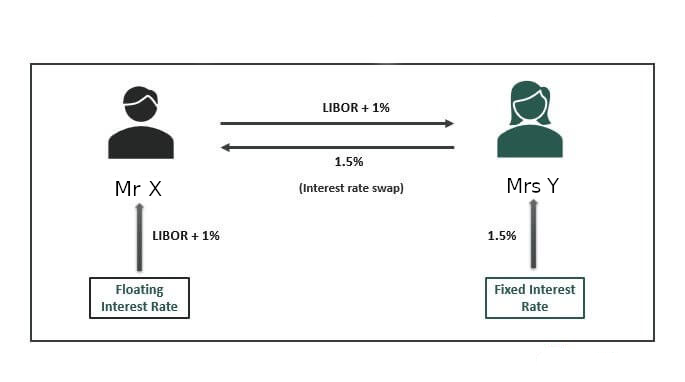
\includegraphics[width=0.9\linewidth]{images/Interest-Rate-Swap-diagram}
	\end{center}
\end{frame}

\begin{frame}{IRS as Sum of FRA}
	\begin{itemize}
		\item The swap payoff in \cref{eq:payoff_payer_irs} can be re-interpreted as a portfolio of FRAs.
		\item Indeed consider a \emph{Receiver IRS} and express its payoff as a sum of FRAs using \cref{eq:fra_payoff_withF}
		\begin{equation*}
			\begin{aligned}
				&\textbf{RFS}(t,T,\tau,N,K) = N\sum_{i=\alpha+1}^{\beta}\expect{Q}[D(t,T_i)\tau_i(K - L(T_{i-1},T_i))]=\\
				&=N\sum_{i=\alpha+1}^{\beta}\tau_i\cdot P(t,T_i)(K-F(t;T_{i-1},T_i))=
				N\sum_{i=\alpha+1}^{\beta}K\cdot \tau_i\cdot P_i-N\sum_{i=\alpha+1}^{\beta}(P_{i-1}-P_i)=\\
				&=N\sum_{i=\alpha+1}^{\beta}K\cdot\tau_i\cdot P_i-N\cdot[(P_\alpha -\cancel{P_{\alpha+1}}) + (\cancel{P_{\alpha+1}} - \cancel{P_{\alpha+2}}) + \ldots + (\cancel{P_{\beta-1}} - P_{\beta})] \\
			\end{aligned}
		\end{equation*}
	\end{itemize}

	\begin{tcolorbox}[colback=gray!5, colframe=maincolor, arc=0mm, boxrule=0.5pt]
	\footnotesize
	Note that the floating leg of a swap is equivalent to "Long a bond at the start ($T_\alpha$) and Short a bond at the end ($T_\beta$)".
	\end{tcolorbox}
\end{frame}

\begin{frame}{IRS as Sum of FRA}
	\begin{itemize}
		\item The swap payoff in \cref{eq:payoff_payer_irs} can be re-interpreted as a portfolio of FRAs.
		\item Indeed consider a \emph{Receiver IRS} and express its payoff as a sum of FRAs using \cref{eq:fra_payoff_withF}
		\begin{equation}
			\begin{aligned}
				&\textbf{RFS}(t,T,\tau,N,K) = 	N\sum_{i=\alpha+1}^{\beta}\expect{Q}[D(t,S)\cdot\tau_i\cdot(K - L(T_{i-1},T_i))]= \ldots =\\
				&=N\sum_{i=\alpha+1}^{\beta}K\cdot \tau_i\cdot P_i-N\cdot [(P_\alpha -\cancel{P_{\alpha+1}}) + (\cancel{P_{\alpha+1}} - \cancel{P_{\alpha+2}}) + \ldots + (\cancel{P_{\beta-1}} - P_{\beta})] =\\
				&=\boxed{N\sum_{i=\alpha+1}^{\beta}K\cdot\tau_i\cdot P(t,T_i)-N\cdot P(t,T_\alpha)+N\cdot P(t,T_\beta)}\quad\quad\quad\qedsymbol
			\end{aligned}
			\label{eq:swap_as_sum_fra}
		\end{equation}
		\begin{tcolorbox}[colback=gray!5, colframe=maincolor, arc=0mm, boxrule=0.5pt]
		\footnotesize
		Replacing $L(T,S)$ with bond ratios is a robust technique since it doesn't require assuming a specific model yet-it's entirely model-independent.
		\end{tcolorbox}
	\end{itemize}
\end{frame}

\begin{frame}{IRS as Sum of FRA}
	\begin{itemize}
		\item<1-> Even if a swap at inception has a zero NPV, not all the component FRAs will have zero value (\emph{except for the degenerate case of flat forward rates}): some of them will have positive, some other negative NPV; the only constraint being their sum to be zero.
		\item<2-> In a \emph{Payer Swap} with increasing forward rates the first FRAs will have negative value, the last positive.
		\begin{itemize}
			\item If the market doesn't move so much the contract buyer will have to pay a net interest differential in the first part of the contract life, and to receive net interest in the second.
			\item So she will have to fund the first payments then could invest at his best the receipt during the second part. (this is sometimes referred to as the \emph{funding profile of the contract}).
		\end{itemize}
	\end{itemize}

	\uncover<3->{\begin{tcolorbox}[colback=gray!5, colframe=maincolor, arc=0mm, boxrule=0.5pt]
	\footnotesize
	CVA Example: because the Payer, in an upward-sloping curve, \emph{"pays first and receives later"}, a bank actually has a negative exposure in the early years and a positive exposure in later. This makes the timing of a possible counterparty default very important !
	\end{tcolorbox}}
\end{frame}

\begin{frame}[fragile]{An Example \colablink{https://colab.research.google.com/drive/1jjryIuf_E0e51evaYGYpIkjq1ifi5kdt}}
	\begin{columns}
		\column{0.65\linewidth}
		\begin{ipython}
def makePFS(rates):
    vals = []
    today = GlobalConst.OBSERVATION_DATE
    dfs = [1/(1+rates[i])**i for i in range(1, len(rates))]
    dc = DiscountCurve([today+TimeInterval(f"{i}y") for i in range(1, len(rates))], dfs)
    dummy_irs = InterestRateSwap(1, today, "5y", ..., "1y", side=...)
    swap_rate = dummy_irs.swap_rate(dc)
    irs = InterestRateSwap(1, today, "5y", swap_rate, "1y", side=...)
    val, vals = irs.npv_with_FRA(dc)

makePFS([0.05, 0.07, 0.09, 0.11, 0.13, 0.15, 0.17])
makePFS([0.05] * 7)
makePFS(list(reversed([0.05, 0.07, 0.09, 0.11, 0.13, 0.15, 0.17])))
		\end{ipython}
		\begin{center}
		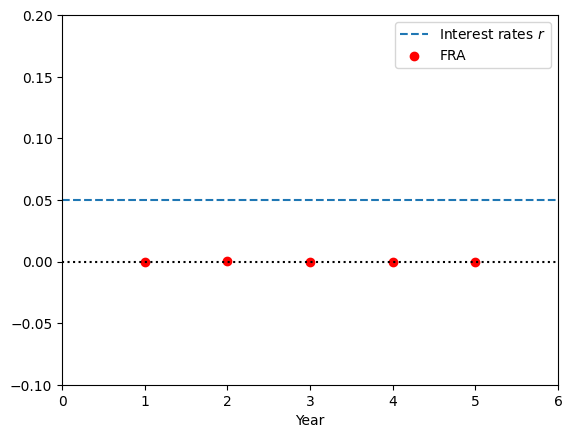
\includegraphics[width=0.42\linewidth]{images/swap_fra_flat.png}
		\end{center}
		\column{0.35\linewidth}
		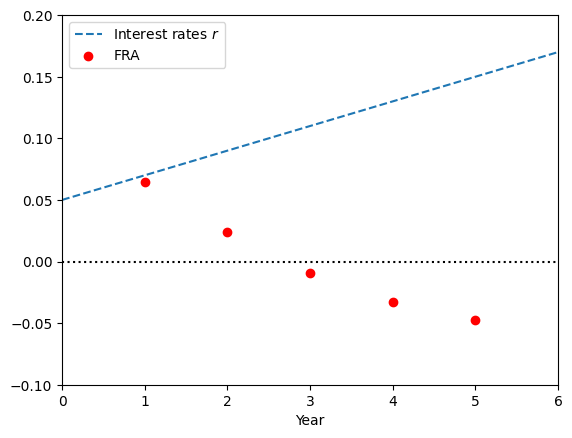
\includegraphics[width=0.82\linewidth]{images/swap_fra_up.png}\\
		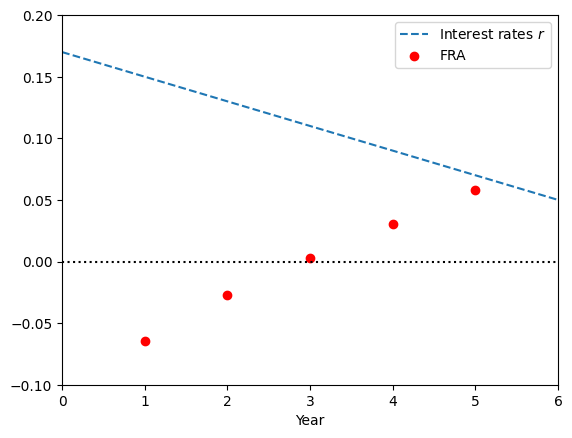
\includegraphics[width=0.82\linewidth]{images/swap_fra_down.png}
	\end{columns}
\end{frame}

\begin{homework}
	\begin{frame}{\textcolor{white}{Homework}}
		\begin{itemize}
			\item[white] Assume that company A has agreed to pay a 6-month Libor and receive a fixed interest rate of 8\% per annum (with interest payable every six months) from the face value of 100 million. Swap is 1.25 years to expire. The interest rates for 3, 9 and 15 months are: 10\%, 10.5\% and 11\% respectively. Assume that interest rates are continously compounded. The 6-month Libor is currently 10.2\%. Calculate the value of this swap for company A. Determine the value of the swap using the relationship between interest rate swap and FRA.
			\item[white] Which of the following strategies is (are) appropriate ?
			\small{
				\begin{itemize}
					\item[white] If a borrower has a fixed rate debt and is expecting interest rates to rise, then the borrower should not enter into a swap.
					\item[white] If an investor has floating rate assets and is expecting interest rates to rise, then the investor should enter into a receiver swap.
					\item[white] If a borrower has floating rate debt and is expecting interest rates to rise, then the borrower should enter into a payer swap.
					\item[white] If an investor has fixed income assets and is expecting interest rates to drop, then the investor should enter into a payer swap.
			\end{itemize}}
		\end{itemize}
	\end{frame}
\end{homework}

\subsection{Swap Rate}
\begin{frame}{Swap Rate as Break-Even Rate}
	\begin{block}{Definition}
		The fixed rate $K$ which makes the swap NPV zero is called \textcolor{maincolor}{forward swap rate}:
		\begin{equation}
			S_{\alpha,\beta}(t) = \frac{P(t, T_\alpha)-P(t,T_\beta)}{\sum_{i=\alpha+1}^{\beta}\tau_i P(t,T_i)} = \frac{P(t, T_\alpha)-P(t,T_\beta)}{A_{\alpha,\beta}(t)}
		\end{equation}
		where it has been defined the \textcolor{maincolor}{annuity} as  $A_{\alpha,\beta}(t) = \sum_{i=\alpha+1}^{\beta} \tau_i P(t, T_i)$.

		If $T_\alpha=0$ we have the \textcolor{maincolor}{spot swap rate}.
		Notice the swap rate makes the contract fair at inception by definition.
	\end{block}
\end{frame}

\begin{frame}{Swap Payoff Alternative Expression}
	\begin{itemize}
		\item<1-> Consider a Payer IRS with $N=1$ for simplicity (using \cref{eq:swap_as_sum_fra})
		\begin{equation*}
			\textbf{PFS} = P(t,T_\alpha)-P(t,T_\beta)-\sum_{i=\alpha+1}^{\beta}K\cdot\tau_i\cdot P(t,T_i)
		\end{equation*}
		\item<2-> By multiplying and dividing by the \textcolor{maincolor}{annuity}
		we get
		\begin{equation}
			\begin{gathered}
				\textbf{PFS}=\frac{A}{\sum\tau_iP(t, T_i)}\left[P(t,T_\alpha)-P(t,T_\beta)-K\sum_{i=\alpha+1}^{\beta}\tau_i P(t,T_i)\right]=\\
				= \boxed{A (S_{\alpha,\beta}(t)-K)}
			\end{gathered}
			\label{eq:swap_payoff_with_swap_rate}
		\end{equation}
		(\textbf{note:} this expression will be useful when pricing swaptions).
	\end{itemize}
\end{frame}

\begin{homework}
	\begin{frame}{\textcolor{white}{Homework}}
		\begin{itemize}
			\item[white] A bank enters into a 2-year Payer Interest Rate Swap with a notional $N=\$10,000,000$. The swap has annual payments ($\tau =1.0$). You are given the following market prices for Zero-Coupon Bonds (ZCBs) today ($t=0$):
			\begin{itemize}
				\item[white] 1-year ZCB price: $P(0,1)=0.9850$;
				\item[white] 2-year ZCB price: $P(0,2)=0.9600$.
			\end{itemize}
			Calculate the Annuity Factor ($A_{0,2}$) for this swap and the Par Swap Rate ($S_{0,2}$).
			Finally	calculate the 1-year Forward Libor rate $F(0;1,2)$ and show that the Par Swap Rate is indeed a weighted average of the forward rates.
		\end{itemize}
	\end{frame}
\end{homework}

\begin{frame}{Swap Curve}
	\begin{itemize}
		\item The \emph{swap curve} is a graphical representation of the relationship between the fixed interest rate and the IRS maturity (typically ranging from 1 to 30 years).
		\item These swap rates are determined through market transactions, reflecting the market's consensus on future interest rate expectations.
		\begin{columns}
			\column{0.45\linewidth}
			\begin{center}
				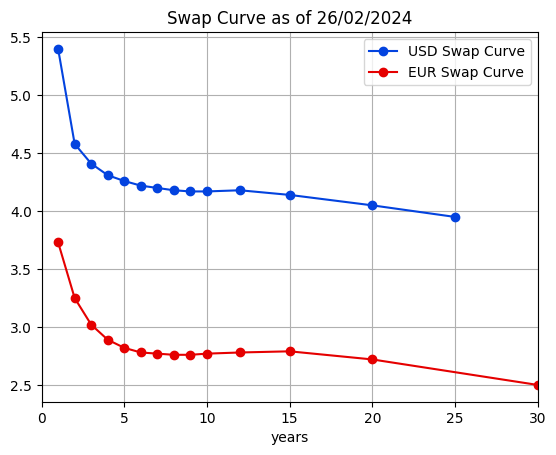
\includegraphics[width=1\linewidth]{images/swap_curve}
			\end{center}
			\column{0.55\linewidth}
			\small{
				\item An upward-sloping \emph{(normal)} curve indicates longer-term interest rates are higher than short-term rates (expectations of economic growth and inflation).
				\item A downward-sloping \emph{(inverted)} curve suggests short-term rates are higher than long-term rates (potential economic downturns or market uncertainties).}
	\end{columns}
%	\item Swap rates are often used as benchmarks for pricing other financial instruments, such as corporate bonds and loans.
\end{itemize}
\end{frame}

\begin{frame}{Yield vs Swap Curve}
\begin{itemize}
	\item Several factors can impact swap curve movements (changes in interest rates, market sentiment, economic indicators, central bank policies\ldots).
	\item One way to interpret it is through the \textbf{Swap Spread} = $S_{\alpha,\beta}(t) - \text{Yield}_{\text{Govt Bond}}$.
%	\item Since the swap curve reflects exchanged rates over various time horizons, it offers a more accurate representation of market expectations and risk perceptions, as it is based on actual transactions.
	\begin{columns}
		\column{0.55\linewidth}
		\item \textbf{Credit Component:} Reflects the perceived risk of the interbank sector (AA-rated banks) vs. the Sovereign.
		\item \textbf{Liquidity Component:} Swaps are often more liquid than specific bond issues, making the swap curve a smoother benchmark for "market expectations."
		\column{0.40\linewidth}
		\begin{center}
			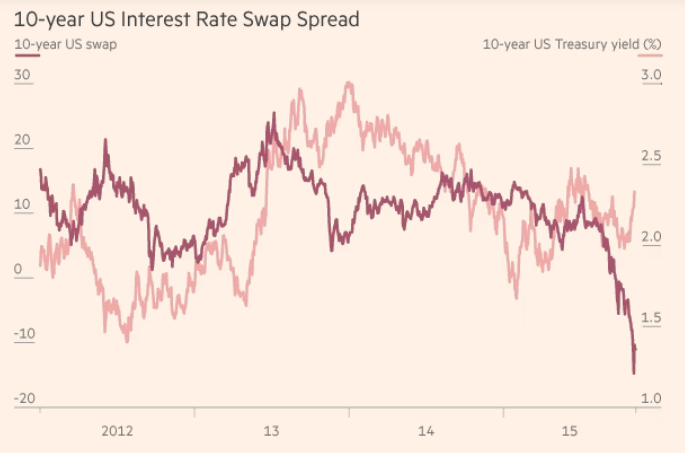
\includegraphics[width=1.\linewidth]{images/swap_spread}
		\end{center}
	\end{columns}
	\item A negative swap spread was once considered an "impossible" anomaly, but it has become a frequent reality since the 2008 crisis.
	\item Supply and Demand Imbalances is the most significant driver. If a government issues a massive amount of bonds to fund a deficit, the market becomes "flooded". High supply lowers the price of Treasuries, which pushes Treasury yields up.
\end{itemize}
\end{frame}

\begin{homework}
	\begin{frame}{\textcolor{white}{Homework}}
		\begin{itemize}
			\item[white]In a stochastic interest rate framework prove that the price of a Zero-Coupon Bond $P(t,T)$ is strictly greater than the exponential of the expected integrated short rate.
			Explain the financial intuition behind this 'paradox' and its implications for convexity adjustments."
			
			Provide a numerical example for the result.
			
			\textbf{Hint}: use Jensen's inequality
		\end{itemize}
	\end{frame}
\end{homework}

\subsection{Swap and Bond Switching}

\begin{frame}{Swap-Bond Equivalence}
	\begin{itemize}
		\item A Swap is effectively an exchange of two bonds with the same notional N:
		\begin{equation*}
			\textbf{PFS}(t) = \underbrace{N(P(t,T_\alpha)-P(t,T_\beta))}_{\text{Floating Leg (FRN)}} - \underbrace{NK \sum_{i=\alpha+1}^{\beta} \tau_i P(t,T_i)}_{\text{Fixed Leg (Coupon Stream)}}
		\end{equation*}
		\item Financial Interpretation:
		\begin{itemize}
			\item The \textcolor{maincolor}{Fixed Leg} is a stream of fixed coupons.
			\item The \textcolor{maincolor}{Floating Leg} is a Floating Rate Note (FRN) coupon stream (excluding the final principal).
		\end{itemize}
		\item No-Arbitrage: a Payer Swap is equivalent to being \textbf{Short a Fixed Rate Bond} and \textbf{Long a Floating Rate Note}.
	\end{itemize}
\end{frame}

\begin{frame}{Valuing the Floating Rate Note (FRN)}
	\begin{itemize}
		\item Consider an FRN paying EURIBOR at dates $\{T_{\alpha+1},\ldots,T_\beta\}$, plus the notional $N$ at $T_\beta$.
		\item Use the telescoping sum of Forward Rates to valuate the contract.
		\begin{equation*}
			\begin{aligned}
				\textbf{FRN}(t) &= \text{PV(Coupons)} + \text{PV(Principal)} \\
				&= N\cdot(P(t,T_\alpha) - P(t,T_\beta)) + N\cdot P(t,T_\beta) \\
				&= \boxed{N\cdot P(t, T_\alpha)}
			\end{aligned}
		\end{equation*}
		\item If $t=T_\alpha$ \textbf{(reset date)}, then $P(T_\alpha,T_\alpha)=1$ and $\textbf{FRN}=N$.
		\item \textit{"An FRN always trades at par on its reset dates."}
	\end{itemize}
\end{frame}

\begin{frame}{The "Sawtooth" Behavior of FRN Prices \colablink{https://colab.research.google.com/drive/114sF_max6lAIHDjaSz55O9TrJODH9Hei}}
	Between reset dates, the FRN price is determined by the next coupon ($C_{\text{fixed}}$) already fixed:
	\begin{equation*}
		\text{FRN}(t) = P(t, T_{\text{next}}) \cdot (N + C_{\text{fixed}})
	\end{equation*}

	\begin{columns}[T]
		\begin{column}{0.5\linewidth}
			Price Evolution:
			\begin{itemize}
				\item Right \textbf{after} a reset: the bond trades at par ($N$).
				\item \textbf{Towards} a reset: the price rises as the coupon "accrues."
				\item Right \textbf{before} payment: $\text{Price} = N + C$.
			\end{itemize}
		\end{column}

		\begin{column}{0.5\linewidth}
			\begin{center}
				% Ensure the image path is correct or use a placeholder
				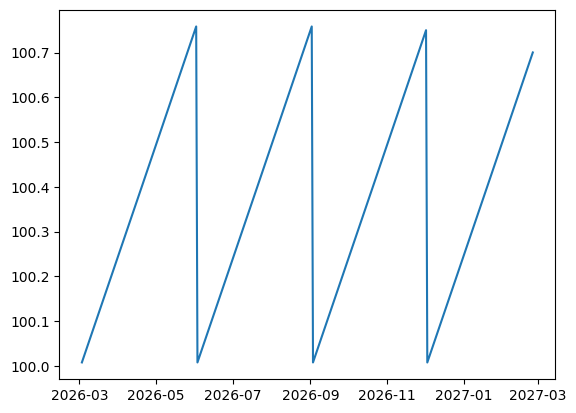
\includegraphics[width=0.9\linewidth]{images/frn_sawtooth}
			\end{center}
		\end{column}
	\end{columns}
\end{frame}

\begin{frame}{A Counterexample}
	\begin{itemize}
		\item<1-> \emph{"Why did Italian CCTs trade below par in 2011 even though they are FRNs ?"}
		\item<2-> An FRN trades at par only if the coupon is exactly equal to the discount rate.
		\item<2-> In 2011, the market became extremely worried about Italy's ability to repay its debt. This added a Credit Spread to the required return.
		\item<2-> The bond was "locked" into paying a small spread, but the market now demands a huge spread.
		\item<2-> To make up for the fact that the coupon is "too low" compared to the new risk, the Price must drop below 100.

\begin{equation*}
	P = \sum_{i=1}^{n}\left(\frac{(L_i+s)\tau_i}{1+r_i\tau_i}\right) + \cdots \xrightarrow{r_i = L_i+s} \text{ Trade at Par}
\end{equation*}

\begin{equation*}
	P = \sum_{i=1}^{n}\left(\frac{(L_i+s)\tau_i}{1+(L_i+s+\gamma)\tau_i}\right) + \cdots \xrightarrow{\text{credit spread $\gamma$}} \text{ Trade below Par}
\end{equation*}
%
%		Because the market perceived a Credit Spread over EURIBOR. The "at par" proof assumes we discount at the same rate the bond pays. If the Issuer's risk increases, the bond trades at a discount (Price $<$ Par).
%
%
%
%
%		The Coupon: CCTs typically paid a coupon linked to the 6-month BOT (Treasury Bill) or Euribor. This "spread" over the base rate was fixed when the bond was issued (often close to zero or very small).
%
%		As the crisis hit, investors demanded a much higher return to compensate for the risk of default. They wanted Euribor+500 basis points.
%
	\end{itemize}
\end{frame}


\section{Economic Intuition: Why Banks Use Swaps}

\begin{frame}{Trading and Hedging Strategies}
	\begin{itemize}
		\item Directional Bets
		\begin{itemize}
			\item \textbf{Payer Swap:} effectively a "short" position. You profit when rates rise because the fixed rate you pay is lower than the new market equilibrium.
			\item \textbf{Receiver Swap:} effectively a "long" position. You profit as rates fall because your locked-in fixed coupon becomes more valuable.
		\end{itemize}

		\item Curve Trades
		\begin{itemize}
			\item \textbf{Steepener} (Long the Spread): pay 30Y / receive 10Y.
			\begin{itemize}
				\item \textit{Rationale:} expectation of rising inflation or increased fiscal supply at the long end.
				\item \textit{P\&L:} profit if $(L_{30y} - L_{10y})$ increases.
			\end{itemize}
			\item \textbf{Flattener} (Short the Spread): receive 30Y / pay 10Y.
			\begin{itemize}
				\item \textit{Rationale:} expectation of aggressive central bank tightening (lifting the short/belly) or a looming recession (lowering long-term growth expectations).
				\item \textit{P\&L:} profit if the 30Y rate falls relative to the 10Y.
			\end{itemize}
		\end{itemize}
	\end{itemize}
\end{frame}

\begin{frame}{The Financing Dilemma: Fixed vs. Floating}
	\begin{itemize}
		\item Imagine \textit{MyFavouriteBank} needs to raise $\$N$ in the market.
		\item At inception ($t=0$), two strategies are NPV-equivalent:
		\begin{enumerate}
			\item \textbf{Floating Strategy:} issue a FRN paying EURIBOR;
			\item \textbf{Fixed Strategy:} issue a Coupon Bond paying $K=S_{\alpha, \beta}$ (the Swap Rate).
		\end{enumerate}
		\item The bank selects based on \textbf{both} its \textcolor{maincolor}{Asset Liability Management} needs and investor demand.
	\end{itemize}
\end{frame}

\begin{frame}{Asset-Liability Matching (ALM)}
	\begin{itemize}
		\item \textbf{The Retail Paradox:} individuals dislike floating rates because salaries are fixed.
		\item \textbf{The Bank Perspective:} banks, instead, often prefer \textbf{floating liabilities} to match their \textbf{floating assets} (commercial loans).
		\item Imagine a scenario with increasing interest rates:
		\begin{itemize}
			\item \textbf{Liability Side:} the bank pays higher coupons to bondholders;
			\item \textbf{Asset Side:} the bank earns higher interest from its loan portfolio;
			\item \textbf{Result:} the Net Interest Margin remains stable.
		\end{itemize}
		\item This "natural hedge" is the essence of bank risk management.
	\end{itemize}
	\begin{tcolorbox}[colback=gray!5, colframe=maincolor, arc=0mm, boxrule=0.5pt]
		\footnotesize
		The Swap as a Transformation Tool: as said many investors (Insurance, Pension Funds) demand fixed coupons for long-term certainty. The bank issues a Fixed Rate Bond to satisfy investors. Then it enters a \textbf{Payer Swap}. The \emph{"Received Fixed"} leg cancels the \emph{"Fixed Coupon"} of the bond. The bank is left with a synthetic Floating Rate Liability.
	\end{tcolorbox}
\end{frame}

\subsection{Basis Swaps}
\begin{frame}{What is a Basis Swap?}
	\begin{itemize}
	\item A \textcolor{maincolor}{Basis Swap} exchanges two floating legs with different tenors (e.g., EURIBOR 3M vs. EURIBOR 6M).
	\item One leg is paid "flat," while a \textcolor{maincolor}{spread $s$} is added to the other (usually the shorter tenor) to make the NPV zero at inception.
	\end{itemize}
	\begin{center}
		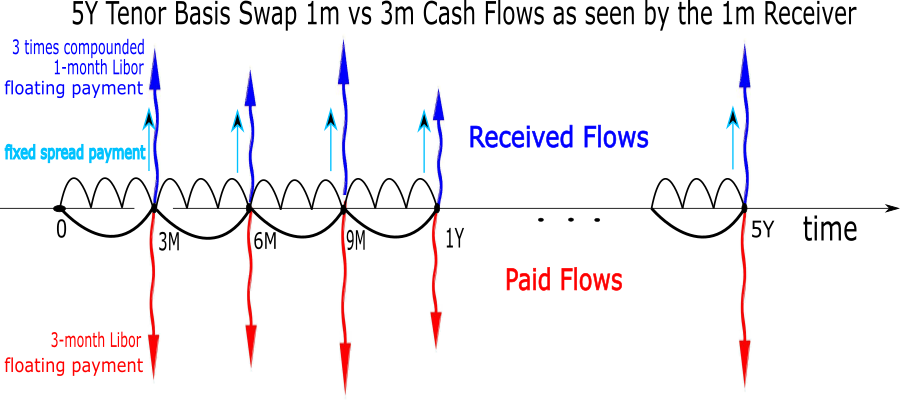
\includegraphics[width=0.6\linewidth]{images/tenor_basis_swap}
	\end{center}
\end{frame}

\begin{frame}{Basis Swap Valuation}
	\begin{itemize}
		\item A Basis Swap can be priced according to the following expression
		\begin{equation}
			\begin{aligned}\textbf{TBS}(t) = \sum_{i=1}^n \tau_i^{L} F^{L}&(t;T_{i-1},T_i)P(t,T_i) - \\
			&-\sum_{j=1}^m \tau_j^{S} (F^{S}(t;T_{j-1},T_j)+\textcolor{maincolor}{s})P(t,T_j)
			\end{aligned}
		\end{equation}
		where $L$ (long index) denotes the index with the longer tenor and $S$ (short index) the other with the shorter tenor.

		\item Basis Swaps usually quote at par, meaning that the price of the swap is zero and that the present value (PV) of each of the traded legs is the same, due to the basis spread.
	\end{itemize}
\end{frame}

\begin{frame}{Single Curve Framework Paradox}
	\begin{itemize}
		\item In the pre-2008 framework, any floating leg (assuming no credit risk) was worth:
		\begin{equation*}
			\text{Value} = P(t, T_\alpha) - P(t, T_\beta)
		\end{equation*}
		\item If both legs started at $T_\alpha$ and ended at $T_\beta$, their values had to be identical (telescoping sum).
		\item E.g. if Leg3M=Leg6M, then the basis spread $s$ should always be zero.
		\item Formally a couple of assumptions must hold: reinvestability at the same risk-free rate, and that the Forward Rate is perfectly consistent with the Zero-Coupon Bond prices (i.e., $F(t;T_1,T_2)=1/\tau(P_2/P_1-1)$).
		\item In reality the market treats a 6-month loan as riskier than two consecutive 3-month loans. This difference reflects Credit and Liquidity Risk that the single-curve model ignores.
	\end{itemize}
\end{frame}

\begin{frame}{The Post-Crisis Shift: Multi-Curve Pricing}
	\begin{itemize}
		\item Today, we no longer use one curve. We use:
		\begin{enumerate}
			\item \textbf{Discounting Curve:} Usually the OIS (Overnight Index Swap) curve (risk-free).
			\item \textbf{Forward Curves:} Separate curves for each tenor (3M, 6M, 12M).
		\end{enumerate}
		\item \textbf{The spread $s$} represents the market's preference for liquidity. In times of stress, the spread between 3M and 6M widens significantly as banks become reluctant to lend for longer periods.
	\end{itemize}

\end{frame}

\section{Credit Risk and Asset Swap}

\begin{frame}{The Impact of Credit Risk}
	\begin{itemize}
		\item In the real world, entities (Banks/Corporates) pay a \textcolor{maincolor}{credit spread} over the risk-free rate (EURIBOR/OIS).
		\item A "Risky" Issuer must offer higher yields to attract investors:
		\begin{enumerate}
			\item \textbf{Fixed Bond:} a higher coupon $K_{risky} > S_{\alpha,\beta}$;
			\item \textbf{Floating Bond:} a spread over the variable rate ($L+s$).
		\end{enumerate}
		\item To hedge interest rate risk, a bank often swaps its fixed-rate risky debt into floating, leading to the Asset Swap structure.
	\end{itemize}
\end{frame}

\begin{frame}{Par Asset Swap: The Synthetic FRN}
	\begin{itemize}
		\item An \textcolor{maincolor}{Asset Swap (AS)} transforms a risky fixed-rate bond into a synthetic floating-rate note, keeping the credit risk profile unchanged.
		\item The Package:
		\begin{enumerate}
			\item purchase a risky bond at market price $\overline{\text{CBP}}$.
			\item enter into an Interest Rate Swap to exchange fixed coupons for $L+s_{AS}$.
		\end{enumerate}
		\item At $t=0$, the buyer pays exactly \textbf{Par (100\%)}:
		\begin{itemize}
			\item if Bond price $\overline{\textbf{CBP}}<1$: buyer pays 1 total (Bond + upfront to seller);
			\item if Bond price $\overline{\textbf{CBP}}>1$: buyer pays 1 total (Bond - upfront from seller).
		\end{itemize}
	\end{itemize}
	
\end{frame}

\begin{frame}{Asset Swap: Strategic Motivations \& Players}
	\begin{itemize}
		\item Why consider an Asset Swap ?
		\begin{itemize}
			\item \textcolor{maincolor}{Interest Rate Risk Decoupling}: isolate credit risk by hedging out the underlying interest rate duration.
			\item \textcolor{maincolor}{Yield Enhancement}: access credit spreads in a floating-rate format that may offer higher returns than standard FRNs.
			\item \textcolor{maincolor}{Customization}: synthetically create a security with a specific maturity or seniority that does not exist in the cash FRN market.
		\end{itemize}
		
		\item Who are the key participants ?
		\begin{itemize}
			\item \textbf{Banks \& Treasury Desks}: to manage \textit{Asset-Liability Mismatch} (ALM) by converting fixed-rate assets to floating to match their funding base ($L + \text{spread}$).
			\item \textbf{Institutional Investors}: insurance companies or pension funds looking to capture the "excess spread" of a specific corporate bond without the rate volatility.
			\item \textbf{Arbitrageurs}: to exploit mispricings between the cash bond market and the Credit Default Swap (CDS) market (the \textit{Basis Trade}).
		\end{itemize}
		
		\item The Core Objective:
		\begin{itemize}
			\item Transform a \textbf{directional} bet on interest rates into a \textbf{pure credit play} on the issuer.
		\end{itemize}
	\end{itemize}
\end{frame}

\begin{frame}{Transforming the Risk Profile}
	Imagine you believe \emph{SolidCompany} won't default anytime soon, but you are terrified that the ECB will hike interest rates, causing bond prices to crash.
	
	\begin{table}[]
		\centering
		\scriptsize
		\begin{tabular}{|p{2cm}|p{6cm}|p{6cm}|}
			\hline
			\textbf{Scenario} & \textbf{Fixed-Rate Bond} (4\%) & \textbf{Asset Swap} Pay Fixed 4\% / Receive $Euribor + 1.50\%$ \\ \hline
			Rates Rise $+2\%$ & Bond Price Crashes. You are stuck with a low yield. & No Impact. Your income rises automatically with Euribor. \\ \hline
			Rates Fall $-2\%$	 & Bond Price Soars. You gain on duration. & No Impact. Your income falls, but stays 1.5\% above market. \\ \hline
			Credit Quality Improves & Bond price rises slightly. & ASW Spread tightens. The value of your package increases. \\ \hline
			Credit Quality Worsens & Bond price falls. & ASW Spread widens. The value of your package decreases. \\ \hline
		\end{tabular}
	\end{table}
	
	\begin{itemize}
		\item \textbf{Neutralization}: the \textcolor{maincolor}{Interest Rate Risk} (Macro) is cancelled out by the swap leg.
		\item \textbf{Isolation}: investor left with \textbf{Credit Play} (Micro) on SolidCompany to pay Euribor + s.
		\item \textbf{Suitability}: best for investors "Bullish" on issuer, "Bearish" on market environment.
	\end{itemize}
\end{frame}

\begin{frame}{Valuation of the Asset Swap}
	\begin{center}
		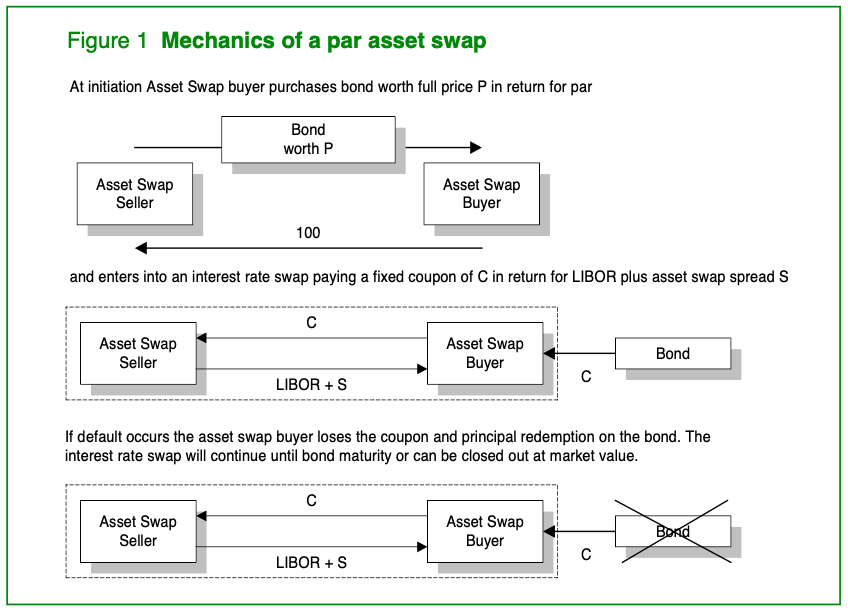
\includegraphics[width=0.7\linewidth]{images/asset_swap}
	\end{center}
\end{frame}

\begin{frame}{Valuation of the Asset Swap}
	\begin{itemize}
		\item From the perspective of the Asset Swap seller the value of the package is given by (we are considering spot trading so $T_\alpha = t = 0$)
		\begin{equation}
			\begin{aligned}
				\textbf{AS}=1&-\overline{\textbf{CBP}}+K\sum_{i=1}^{\beta}\tau_i P(0,T_i)-\sum_{i=1}^{\beta}\tau_i P(0,T_i)(L(T_{i-1},T_i)+s) =\\
				=1&-\overline{\textbf{CBP}}+K\sum_{i=1}^{\beta}\tau_i P(0,T_i)\\
				&-\sum_{i=1}^{\beta}\tau_i P(0,T_i)L(T_{i-1},T_i)-\sum_{i=1}^{\beta}\tau_i P(0,T_i)s=0
			\end{aligned}
			\label{eq:asset_swap_value}
		\end{equation}
	\end{itemize}
\end{frame}

\begin{frame}{Valuation of the Asset Swap}
	\begin{itemize}
		\item We can replace the future rates with the forward rates definition in terms of ZCB, and by its definition (\cref{eq:forward_rate_definition})
		\begin{equation*}
			\begin{aligned}
				\sum_{i=1}^\beta &\tau_i P(0,T_i)F(t;T_{i-1},T_i) =  \sum_{i=1}^\beta \cancel{\tau_i P(0,T_i)}\frac{P(0,T_{i-1})-P(0,T_i)}{\cancel{\tau_i P(0,T_i)}} = \\
				= &P(0,0) \cancel{- P(0,T_1)} + \cancel{P(0,T_1)} \cancel{- P(0,T_2)} + \cancel{P(0,T_2)} + \\
				&\ldots \cancel{- P(0, T_{\beta-1})} \cancel{+ P(0, T_{\beta-1})}-P(0,T_\beta) = 1-P(0,T_\beta)
			\end{aligned}
		\end{equation*}
		\item Substitute into \cref{eq:asset_swap_value} to get
		\begin{equation*}
			\begin{aligned}
				\textbf{AS}=1&-\overline{\textbf{CBP}}+K\sum_{i=1}^{\beta}\tau_i P(0,T_i) -(1-P(0,T_\beta))
				+ \sum_{i=1}^\beta\tau_i P(0,T_i)s=0
			\end{aligned}
		\end{equation*}
	\end{itemize}
\end{frame}

\begin{frame}{Valuation of the Asset Swap}
	\begin{itemize}
		\item Canceling out the 1s
		\begin{equation*}
			\textbf{AS}=-\overline{\textbf{CBP}}+K\sum_{i=1}^\beta\tau_i P(0,T_i) + P(0,T_\beta) + \sum_{i=1}^{\beta}\tau_i P(0,T_i)s=0
		\end{equation*}
		\item Finally we know that
		\begin{equation*}
			\textbf{CBP} = P(0,T_\beta) + K\sum_{i=1}^\beta\tau_i P(0,T_i)
		\end{equation*}
		represents the price of coupons and principal of a  risk-free bond which can be denoted by \textbf{CBP}.
		\item Solving for $s$ we arrive at the final expression
		\begin{equation}
			\boxed{s = \frac{\textbf{CBP}-\overline{\textbf{CBP}}}{\sum_{i=1}^{\beta}\tau_iP(0,T_i)} =  \frac{\textbf{CBP} - \overline{\textbf{CBP}}}{A_{\alpha,\beta}(0)}}
		\end{equation}
		\myendproof
	\end{itemize}
\end{frame}

\begin{frame}[fragile]{ASWP Spread and Default Probability \colablink{https://colab.research.google.com/drive/1I6hgddp0yYaVRWlQ0ltZQvgErERDE-zX}}
	Consider ASWP on a 5Y fixed rate bond (yearly coupons 3\%). If the counterparty has nonull default probability, let's see how ASWP spread varies.
	
	\begin{columns}
		\column{0.5\linewidth}
		\begin{ipython}
			import numpy as np
			
			pds = np.arange(0, 1.0, 0.01)
			
			bond = FixedRateBond(today, 0.03, "5y", "1y", 100)
			asw = ParAssetSwap(bond)
			
			spreads = []
			prices = []
			for pd in pds:
			market_price_bond = bond.npv_default(dc, pd=pd, R=0.4)
			prices.append(market_price_bond)
			spreads.append(asw.asspread(dc, pd))
		\end{ipython}
		\column{0.5\linewidth}
		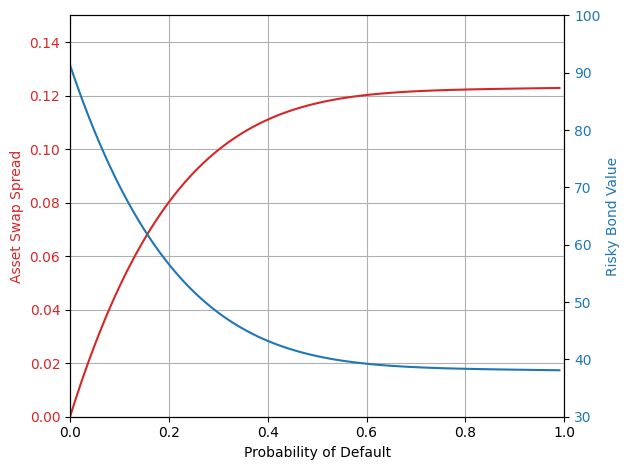
\includegraphics[width=0.9\linewidth]{images/aswp_spread}
	\end{columns}
\end{frame}

\begin{frame}{AAA-Rated ASW Spread \colablink{https://colab.research.google.com/drive/1I6hgddp0yYaVRWlQ0ltZQvgErERDE-zX}}
	Consider the bond NVIDIA 2030 2.85\% currently yielding 3.99\%. The associated ASW spread can be estimated by $\text{ASWS} = \text{yld} - \text{SOFR}$.
	The curve can be compared to the ASWS for AAA-rated bond estimated as $(\text{OAS} + \text{5y Treasury}) - \text{SOFR}$.
	\begin{center}
		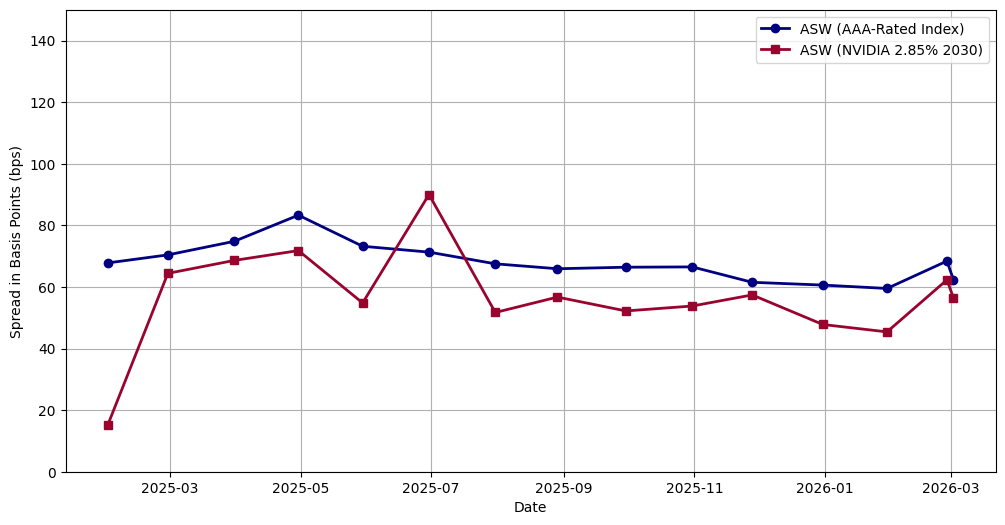
\includegraphics[width=0.75\linewidth]{images/nvidia_spread}
	\end{center}
\end{frame}

\begin{frame}{Why OIS Implies the ASW Spread}
	\begin{itemize}
		\item In an Asset Swap, the investor effectively exchanges fixed coupons for a floating rate (OIS/SOFR). The ASW Spread is the \textbf{residual premium} over OIS that the market demands for holding the bond's credit risk.		
		\[ PV_{\text{Bond}} + \text{Upfront} = PV_{\text{Floating Leg (OIS)}} + PV_{\text{ASW Spread}} \]
		\item Since OIS is nearly risk-free, the gap between the bond's yield and the OIS-based swap rate is the purest measure of the issuer's \textbf{Credit Risk}.
	\end{itemize}
\end{frame}

\begin{frame}{Asset Swap: Credit Considerations}
	\begin {itemize}
	\item A trader may want to hedge anyway the credit risk carried on with the asset swap entering into a \emph{Credit Default Swap (CDS)}.
	\item A CDS is a credit insurance contract where the protection buyer pays \emph{spread} ($s_{CDS}$) and in case of a credit event, the protection seller must pay the contingency payment so that the buyer receives no losses from the default.
\end{itemize}
\begin{center}
	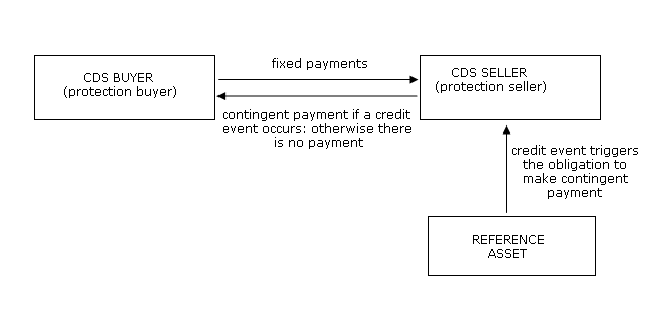
\includegraphics[width=0.7\linewidth]{images/credit-default-swaps}
\end{center}
\end{frame}

\begin{frame}{Hedging Credit: AS vs. CDS \colablink{https://colab.research.google.com/drive/1I6hgddp0yYaVRWlQ0ltZQvgErERDE-zX}}
\begin {itemize}
\item Like $s_{AS}$, also $s_{CDS}$ is quoted on the market, tracking the perceived credit worthiness of the underlying reference entity.
\item In theory, the cost of protecting a bond (CDS) should equal the spread earned for holding it (ASW).
\begin{itemize}
	\item if $s_{AS} - s_{CDS} > 0$ the market pays you more for the risk ($s_{AS}$) than it costs to insure it ($s_{CDS}$). So the investor can buy the bond, financing the purchase, enters in AS and buying protection, making an (almost) risk free profit (\emph{negative basis trading});
	\item if $s_{AS} - s_{CDS} < 0$ can do the opposite.
\end{itemize}
\end{itemize}
\begin{columns}
\column{0.4\linewidth}
The \emph{CDS-Bond Basis} can be estimated considering the HY OAS index and comparing it with CDX.NA.HY.5Y
\column{0.6\linewidth}
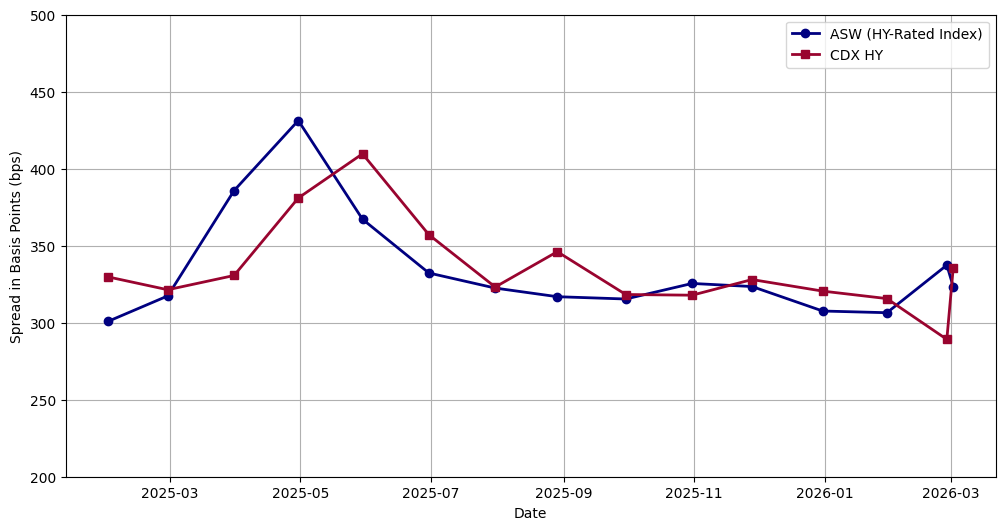
\includegraphics[width=0.85\linewidth]{images/asw_vs_cds}
\end{columns}
\end{frame}

\begin{homework}
\begin{frame}{\textcolor{white}{Homework}}
\begin{itemize}
	\item[white] Describe the asset swap contract for a coupon bond with coupons equal to \textbf{C} and dirty Price equal to $P(t)$. What will happen to the price if the spread increases, all the rest being equal ? What does it mean in term of credit quality expectation by the market for the bond's issuer ?
	\item[white]  Consider the 10-year German Bund DBR 0.5\% 2026 which is currently trading at a clean price of 104.58.
	Given that the 10-year EUR swap rate is 0.44\% what is the par-par asset swap spread for this bond ?
	For this exercise assume that all annuity factors have a value of 10.0 for simplicity.
	\item[white] Consider the 10-year Greek Government Bond GGB 3.0\% 2026 which is currently trading at a clean price of 75.280. Given that the 10-year EUR swap rate is 0.440\% what is the par-par asset swap spread for this bond ?
	\item[white] How does the bond price change with non-zero default probability for the issuer ? Write down the formula for a zero coupon when the issuer has a flat default probability of default $p_{\text{def}}$ and a recovery rate $R$.
	How would you extend it to a fixed coupon bond ?
\end{itemize}
\end{frame}
\end{homework}

\section{Cap and Floor}
\begin{frame}{Caps and Floors}
\begin{itemize}
\item<1-> A \textcolor{maincolor}{Cap} is a Payer IRS in which the payment is done \textcolor{maincolor}{only} if the payoff is positive. Its value results from the expectation of
\begin{equation}
	\expect{Q}_t \left[\sum_{i=\alpha+1}^{\beta}N\cdot\tau_i\cdot D(t,T_i)\max\left[L(T_{i-1},T_i)-K,0\right]\right]
	\label{eq:cap}
\end{equation}
\item<2-> The cap allows investors which have a debt at a variable rate to buy insurance against high rates in the future.
\item<3-> A \textcolor{maincolor}{Floor} is the same kind of object but analogous to a Receiver IRS:
\begin{equation}
	\expect{Q}_t \left[\sum_{i=\alpha+1}^{\beta} N\cdot\tau_i\cdot D(t,T_i)\max\left[K-L(T_{i-1},T_i),0\right]\right]
	\label{eq:floor}
\end{equation}
\end{itemize}
\end{frame}

\subsection{Caplets}
\begin{frame}{Caplet and Floorlet}
\begin{itemize}
\item<1-> Considering each element of the sum in \cref{eq:cap} or \cref{eq:floor} we see that Cap/Floor can be split into forward starting options over a floating rate, called \textcolor{maincolor}{Caplet/Floorlet}.
\item<2-> A Caplet/Floorlet payoff is defined as
\begin{equation*}
	N\cdot\tau_i\cdot D(t,T_i)\max\left[L(T_{i-1},T_i)-K,0\right]
\end{equation*}
and its value is given by
\begin{equation}
	\textbf{Cpl}(t,T_{i-1},T_i,\tau,N,K)=\expect{Q}\left[N\cdot\tau_i\cdot e^{-\int_t^{T_i}r_s ds}(L(T_{i-1},T_i)-K)^+ | \mathcal{F}_t\right]
\end{equation}
\item<3-> This can also be written
\begin{equation*}
	\textbf{Cpl}=N\cdot\expect{Q}\left[\tau_i\cdot e^{-\int_t^{T_{i-1}}r_s ds}\cdot P(T_{i-1},T_i)\cdot  (L(T_{i-1},T_i)-K)^+ | \mathcal{F}_t\right]
\end{equation*}
\end{itemize}
\end{frame}

\begin{frame}{Caplets as ZCB Options}
\begin{itemize}
\item<1-> Using the LIBOR rate definition we get
\begin{equation*}
	\begin{aligned}
		\textbf{Cpl} &=N\cdot\expect{Q}\left[e^{-\int_t^{T_{i-1}}r_s ds}\cdot P(T_{i-1},T_i)\cdot\left(\frac{1}{P(T_{i-1},T_i)}-1-K\tau_i\right)^+ \Big\rvert \mathcal{F}_t\right] \\
		& = N\cdot\expect{Q}\left[e^{-\int_t^{T_{i-1}}r_s ds}\left(1-(1+K\tau_i)\cdot P(T_{i-1},T_i)\right)^+ | \mathcal{F}_t\right]
	\end{aligned}
\end{equation*}
\item<2-> Factoring out $1+K\tau_i$ we finally get
\begin{equation}
	\boxed{\textbf{Cpl}=N\cdot(1+K\tau_i)\cdot\expect{Q}\left[e^{-\int_t^{T_{i-1}}r_s ds}\cdot\left(\frac{1}{1+K\tau_i}-P(T_{i-1},T_i)\right)^+ \Big\rvert \mathcal{F}_t\right]}
\end{equation}
\end{itemize}
\end{frame}

\begin{frame}{Caplets as ZCB Options}
\begin{block}{Intepretation}
\begin{enumerate}
	\item Caplets can be seen as \textcolor{maincolor}{put options} on ZCBs
	\begin{equation*}
		\textbf{Cpl}=N'\cdot\expect{Q}\left[D(t,T_{i-1})\cdot\left(K'-P(T_{i-1},T_i)\right)^+ \Big\rvert \mathcal{F}_t\right]
	\end{equation*}
	\item Similarly floorlets are \textcolor{maincolor}{call options} on ZCBs
	\begin{equation}
		\textbf{Flr}=N'\cdot\expect{Q}\left[D(t, T_{i-1})\cdot\left(P(T_{i-1},T_i)-K'\right)^+ \Big\rvert \mathcal{F}_t\right]
	\end{equation}
\end{enumerate}
\end{block}
It highlights that a Caplet is not just a "rate option" but a Put option on the Bond price. If the bond price drops (rates rise), the Put gains value. This is a very powerful way to link interest rate volatility to bond volatility.
\end{frame}

\section{The Black Model}
\begin{frame}{The Black Model - Overview}
\begin{itemize}
\item The \textcolor{maincolor}{Black Model} extends the Black-Scholes formula to \emph{caplets} (and \emph{swaptions}). 
\item The main difference with respect to the Black-Scholes set up is that \textcolor{maincolor}{forward rates $F(t;T_{i-1},T_i)$ (or swap rates $S_{\alpha\beta}(t)$) are log-normally distributed}, rather than the spot price of the equity underlying.
\item It should be stated that Black’s formulas \emph{did not originally correspond to prices that arise from the application of martingale pricing theory} to some particular model.
\item The advent of the \emph{market models} will provide a belated justification for these formulas but we shall see that the justifications are mutually inconsistent.
\item Indeed, it may be shown that Black’s formulas for caplets and swaptions cannot both hold within the same model.
\end{itemize}
\end{frame}

\begin{frame}{Pricing Caps with the Black-76 Formula}
\begin{block}{Definition}
\begin{equation}
	\begin{aligned}
		\textbf{Cap}_{Bl}(0, \tau,N,K,\sigma_{\alpha,\beta}) &= N\sum_{i=\alpha+1}^{\beta}\textbf{Cpl}_{Bl}(T_i, \tau,K,\sigma_{\alpha,\beta}) = \\ &=N\sum_{i=\alpha+1}^{\beta}\tau P(0,T_i) \textbf{Bl}(K,F(0;T_{i-1},T_i),v_i)
	\end{aligned}
	\label{eq:cap_black}
\end{equation}
where
\begin{equation*}
	\begin{gathered}
		\boxed{\textbf{Bl}(K,F_i,v_i)=F\Phi(d_1(K,F_i,v_i)) - K\Phi(d_2(K,F_i,v_i))} \\
		d_{1,2} = \frac{\log{\cfrac{F_i}{K}} \pm \cfrac{v_i^2}{2}}{v} \\[0.2cm]
		v_i = \sigma_{\alpha,\beta}\sqrt{T_{i-1}}
	\end{gathered}
\end{equation*}
\end{block}
\end{frame}

\begin{frame}{Problems with the Black Model}
\begin{itemize}
\item It is widely used in practice as the metric by which traders translated volatilities into prices until rates became too low and the model collapsed under the assumption of positive rates.
\item In the Black model \textcolor{maincolor}{negative rates are not allowed}.
\begin{equation*}
	d_{1,2} = \frac{\boxed{\log{\frac{F}{K}}} \pm \cfrac{v^2}{2}}{v}
\end{equation*}
but in the last years in the inter-bank market it was not so unusual to find prices for -1\% strike floors.
\item Moreover in the Black model the empirical evidence of the "smile" (volatility vs $K$) is not accounted for, i.e. $\sigma$ is a constant. Two caps identical but for the strike need a different volatility to recover two different market prices if one uses Black formula.
\end{itemize}
\end{frame}

\begin{frame}{The Practitioner Solutions}
\begin{itemize}
\item \textbf{"Smile" issue}: the model is used with \textcolor{maincolor}{different input volatilities for different strikes}. In practice it is a mapping of implied volatilities into prices and vice versa.
\item \textbf{Non-positive rates}: could have switched to a different dynamics, like ABM, where negative values are "normal". But there are large differences in the tails between normal and log-normal distributions.
So Black model has been \textcolor{maincolor}{shifted}. The technique was already known but in the last years became crucial to shift the lower bound of prices admitted by the model.
\end{itemize}
\end{frame}

\begin{frame}{Shifted Log-normal Model \colablink{https://colab.research.google.com/drive/1ZEEw1KP8-e6LL4l17Odoj4GjtlRyQ_I_}}
\begin{itemize}
\item The formula $\textbf{Bl}(K+\alpha,F+\alpha,v_T$) is the standard market fix. By shifting the "zero" floor to $-\alpha$, you allow $F$ to go negative while the argument inside the log stays positive.
\item It can be shown that Black formula provides valid solutions if strike and forward rate are \textcolor{maincolor}{shifted}. For a $(T,S)$ caplet with strike $K$ we get
\begin{equation}
	\textbf{Cpl}_{Bl}(t,T,S,\tau,K,v_T,\alpha) = P(t,S) Bl(K+\alpha,F(t;T,S)+\alpha,v_T)
\end{equation}
where $d_1$ and $d_2$ read as before and instead $v_i$ is now given by
\begin{equation*}
	v_i = \sigma^{\text{shifted}}\sqrt{T_{i-1}}
\end{equation*}
\item The market quotes of $\sigma^{\text{shifted}}$ referred to shifts $\alpha$ of the order of [2\%,3\%].
\end{itemize}
\end{frame}


\section{Swaptions}
\begin{frame}{Swaptions Overview}
\begin{itemize}
\item<1-> The purchaser of an \textcolor{maincolor}{European swaption} has the right but not the obligation to enter into a swap contract, at a given future time, called the \textcolor{maincolor}{swaption maturity}.
\item<2-> There are two types of \textcolor{maincolor}{swaptions} (as the underlying swaps): a \emph{payer} in which at maturity the buyer could become the fixed-rate payer and a \emph{receiver} where she could become the fixed-rate receiver.
\item <3-> \emph{The strike price of the swaption determines the fixed rate of the underlying swap.}
\item<4-> A swaption provides protection for a borrower as it ensures a maximum fixed interest rate payable in the future. Furthermore, it gives her the flexibility, if the rate does not rise above the swaption strike rate at expiry, to choose not to exercise it and take advantage of the lower market rates.
\end{itemize}
\end{frame}

\begin{frame}{Strategic View and Risks}
\begin{itemize}
\item<1-> Usually, the swaption maturity coincides with the first reset date of the underlying IRS (the IRS maturity is called the \textcolor{maincolor}{tenor} of the swaption).
\item<1-> If you are on the buyer side (you are long payer swaption) which is your view on rates ? Why ?
\item<2-> The buyer of a Payer Swaption is Bearish on bond prices (Bullish on rates). They want rates to rise above $K$.
\item<3-> Are there any risks associated with a Swaption?
\begin{itemize}
	\item<4-> The primary risk with a Swaption occurs after you have exercised your right and proceeded with the Swap. Should interest rate movements be different to your expectations, the Swap may have the opposite effect to what you were trying to achieve with the transaction.
	\item<5-> If interest rates do not rise above the strike on the exercise date, you have not obtained any benefit from the premium paid for the purchase of the Swaption. The premium is the cost of obtaining protection against a rise in interest rates.
\end{itemize}
\end{itemize}
\end{frame}

\begin{frame}{Swaption Payoff: The Summation Problem}
\begin{itemize}
\item<1-> The discounted payoff of a payer Swaption (with maturity $T_\alpha$) is given, recalling the value of a payer IRS (\cref{eq:swap_as_sum_fra}) by
\begin{equation}
	\textbf{PSw}=D(t,T_\alpha)\left(\sum_{i=\alpha+1}^\beta \tau_i\cdot P(T_\alpha,T_i) (F(T_\alpha;T_{i-1},T_i) - K)\right)^+
	\label{eq:swaption_payoff_std}
\end{equation}
\item<2-> Unfortunately this payoff \textcolor{maincolor}{cannot} be easily decomposed into elementary parts (as done for Cap/Floor). Indeed the \emph{positive part operator} $(\cdot)^+$ is "outside" the summation (while for Caps it is "inside").
\item<3-> Nevertheless it can be simplified by writing it in a different way...
\end{itemize}
\end{frame}

\begin{frame}{Swaption Payoff}
\begin{itemize}
\item<1-> Recall that the Swap Rate $S_{\alpha,\beta}(t)$ is the rate that sets the NPV of a swap to zero at time $t$. We can express the Payer Swap (PFS) value as:
\begin{equation*}
	\textbf{PFS}(t) = A(t) \left( S_{\alpha,\beta}(t) - K \right)
\end{equation*}
where $A(t)$ is the \textcolor{maincolor}{Annuity} factor.
\item<2-> By modeling the swap rate $S_{\alpha,\beta}(t)$ as the stochastic variable, the Swaption value at time $t$ becomes the expectation of:
\begin{equation}
	\textbf{PSw} = \mathbb{E}^{\mathbb{Q}} \left[ D(t, T_\alpha)\cdot A(T_\alpha)\cdot \max(S_{\alpha,\beta}(T_\alpha) - K, 0) \right]	
	\label{eq:swaption_payoff_annuity}				
\end{equation}
\item<3-> This formulation is intuitive: it is an option on the swap rate, scaled by the value of the fixed-leg cash flows (the annuity).
\end{itemize}
\end{frame}

\begin{frame}{An Example}
\begin{itemize}
\item \textbf{A} has raised a $10y$ loan with floating interest rates fixed every three months (IBOR + margin).
\item \textbf{A} wants to \emph{hedge the loan against rising interest rates but also to benefit from the floating rate}, i.e. should interest rates not rise above a certain level (the swaptions strike-rate $K$).
\item The purchase of a payer swaption could hedge this risk:
\begin{columns}
	\column{0.45\linewidth}
	\begin{itemize}
		\item \textbf{interest rates increase}: \textbf{A} may exercise the swaption and be a party of a swap as a payer of a fixed interest rate;
		\item \textbf{swap-rate below $K$}: it will not be exercised and \textbf{A} will continue to have floating-rate funding.
	\end{itemize}
	\column{0.45\linewidth}
	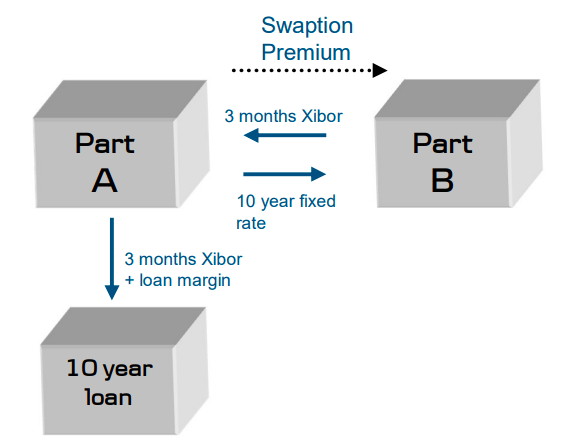
\includegraphics[width=1.\linewidth]{images/swaption_example}
\end{columns}
\end{itemize}
\end{frame}

\begin{homework}
\begin{frame}{\textcolor{white}{Homework}}
\begin{itemize}
	\item[white] In order to hedge your position against interest rate movements which kind of contract would you use:
	\begin{itemize}
		\item[white] a Swap
		\item[white] a Cap/Floor
		\item[white] a Swaption
	\end{itemize}
	List the pros and cons about each one and declare your favourite.
	\item[white] Prove that the difference between the price of a Cap and a Floor with the same strike $K$ and the same maturity structure is equal to the value of a Payer Interest Rate Swap (IRS).
\end{itemize}
\end{frame}
\end{homework}

\begin{frame}{Black Formula for Swaptions}
\begin{itemize}
\item The market standard for pricing European Swaptions is the \textbf{Black-76 formula}, assuming $S_{\alpha,\beta}$ follows a log-normal process.
\item The price of a Payer Swaption is given by:
\begin{equation}
	\boxed{\textbf{PSw}_{Bl} = N \cdot A(0) \left[ S_{\alpha,\beta}(0)\Phi(d_1) - K\Phi(d_2) \right]}
\end{equation}
where:
\begin{equation*}
	\begin{gathered}
		d_{1} = \cfrac{\log\left(\frac{S_{\alpha,\beta}(0)}{K}\right) + \frac{v^2}{2}}{v}, \quad d_2 = d_1 - v \\[0.2cm]
		v = \sigma_{\alpha,\beta}\sqrt{T_\alpha}
	\end{gathered}
\end{equation*}
\item Note: $A(0)$ is the current value of the annuity, and $\sigma_{\alpha,\beta}$ is the \emph{implied volatility} for the specific maturity $T_\alpha$ and tenor $T_\beta - T_\alpha$.
\end{itemize}
\end{frame}

\begin{frame}{Swaptions Volatility Calibration}
\begin{itemize}
\item Swaption volatilities are quoted for different maturities and tenors (length of the underlying swap).
\item Both for ATM and away from ATM on both sides ("swaption smile").
\item The quotes are parametrized according to
\begin{itemize}
	\item maturites;
	\item tenors;
	\item strikes.
\end{itemize}
\item After we have constructed the volatility surface we can fit the smile at each (expiry, tenor) pair.
\end{itemize}
\end{frame}

\begin{frame}{SABR Model}
\begin{itemize}
\item SABR model is the industry standard to model "volatility smile" in the interest rat world. An approximated solution has been given by \emph{Hagan et al.}

\begin{eqnarray} \sigma _{B}(K,f) &=&\frac{\textcolor{red}{\alpha} \left\{ 1+\left[ \frac{\left( 1-\textcolor{red}{\beta} \right) ^{2}}{24}\frac{\textcolor{red}{\alpha} ^{2}}{(fK)^{1-\textcolor{red}{\beta}}}+\frac{1}{4}\frac{\textcolor{red}{\rho \beta \nu\alpha}}{(fK)^{(1-\textcolor{red}{\beta})/2}}+\frac{2-3\textcolor{red}{\rho} ^{2}}{24}\textcolor{red}{\nu}^{2}\right] T\right\} }{(fK)^{(1-\textcolor{red}{\beta})/2}\left[ 1+\frac{(1-\textcolor{red}{\beta})^{2}}{24}\ln ^{2} \frac{f}{K}+\frac{(1-\textcolor{red}{\beta})^{4}}{1920}\ln^{4}\frac{f}{K}\right] } \cdot \frac{z}{\chi (z)} \notag \\ z &=&\frac{\textcolor{red}{\nu}}{\textcolor{red}{\alpha}}(fK)^{(1-\textcolor{red}{\beta})/2}\ln \frac{f}{K};\quad \notag \chi (z) =\ln \left[ \frac{\sqrt{1-2\rho z+z^{2}}+z-\textcolor{red}{\rho}}{1-\textcolor{red}{\rho}}\right] . \notag \end{eqnarray}

\begin{itemize}
	\item $\alpha$: determines the overall level of volatility (the "At-The-Money" level);
	\item $\beta$:determines the backbone of the smile (usually = to 0.5 or 1 to represent log-normal or normal-like behavior);
	\item $\rho$: controls the Skew (slope). A negative $\rho$ creates a downward slope (volatility higher for lower strikes);
	\item $\nu$: controls the Convexity (the "Smile" or curvature).
\end{itemize}
\end{itemize}
\end{frame}

\begin{frame}{SABR Parameters Estimate}
\begin{columns}
\column{0.5\linewidth}
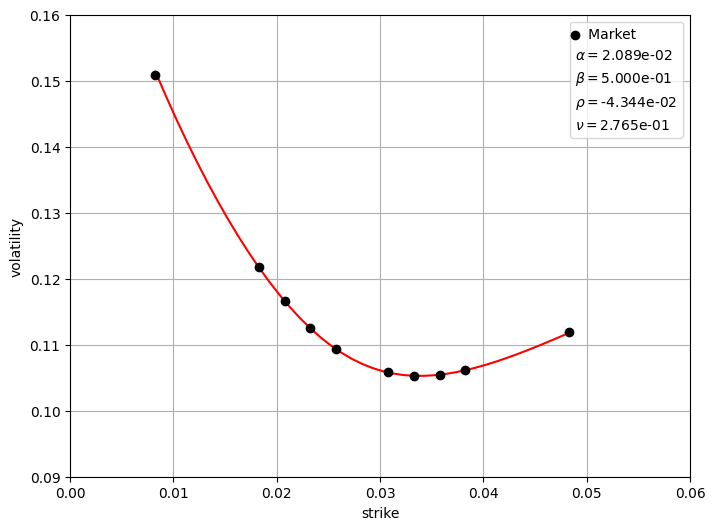
\includegraphics[width=1.\linewidth]{images/10y_10y}
\column{0.5\linewidth}
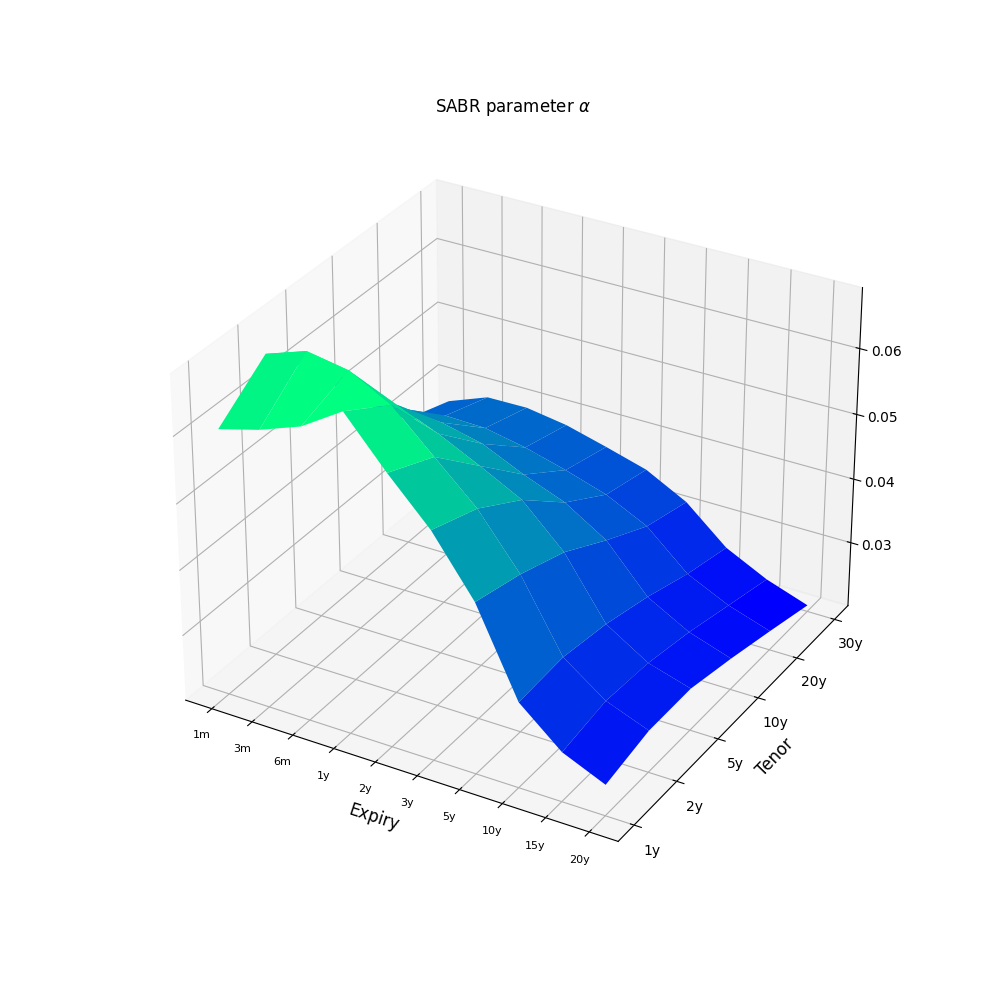
\includegraphics[width=0.45\linewidth]{images/alpha}\\
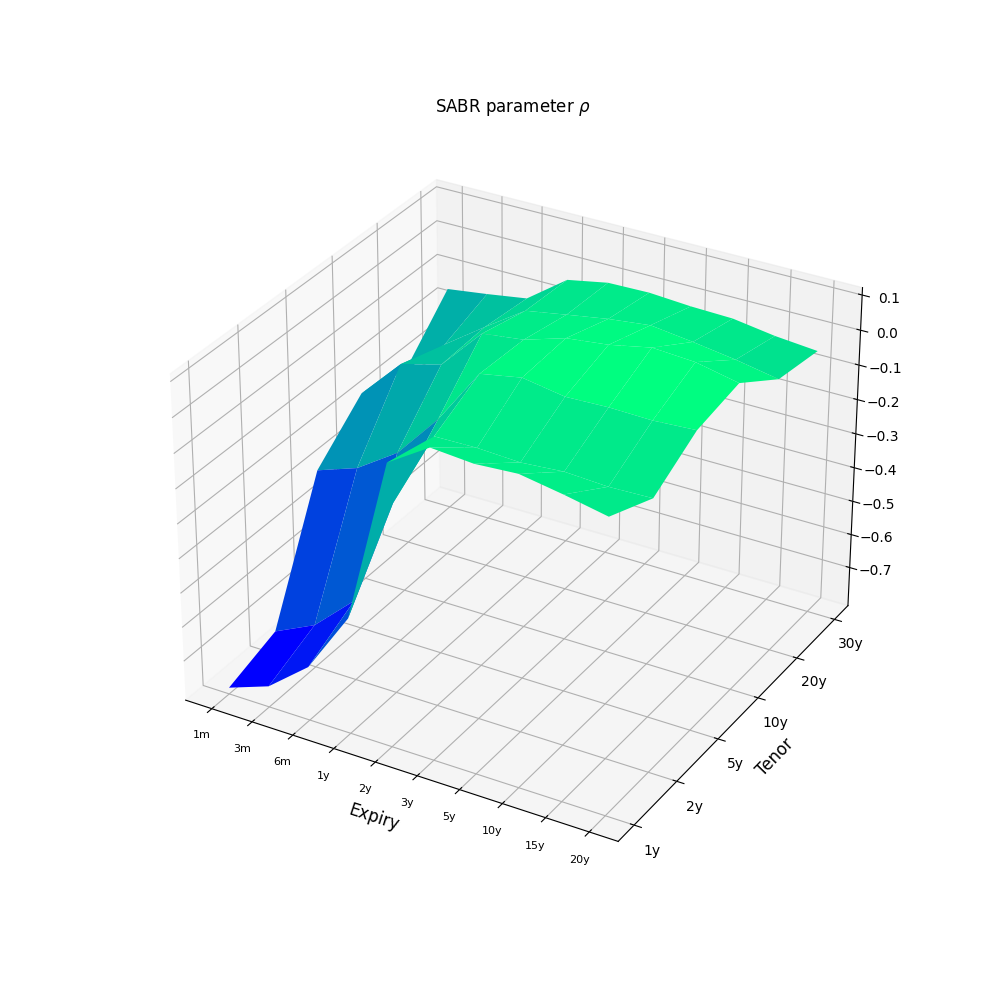
\includegraphics[width=0.45\linewidth]{images/rho}
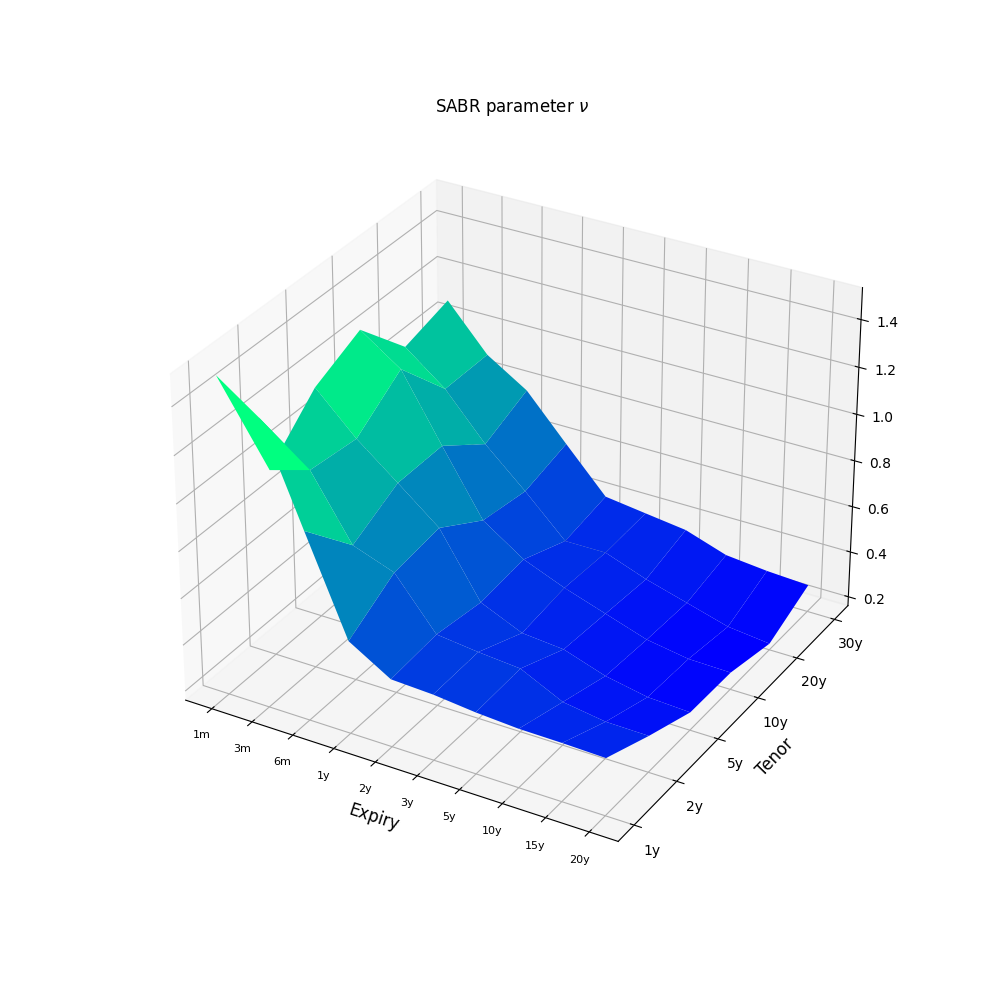
\includegraphics[width=0.45\linewidth]{images/nu}
\end{columns}
\end{frame}

\begin{frame}{Exploiting SABR Model}
\begin{itemize}
\item Smoothing the volatility surface): market swaption data is often "holy"—you might have quotes for 2Y, 5Y, and 10Y tenors, but nothing for 7Y. Use the SABR formula to generate the implied volatility for any strike ($K$). This allows you to price swaptions without "guessing" the volatility.
\item Pricing exotic options: standard calibration usually happens on European swaptions. You can use those parameters to price:
Bermudan Swaptions (use SABR volatility for a Monte Carlo simulation to price options that can be exercised on multiple dates), 
CMS (Constant Maturity Swaps) since SABR is the standard for pricing CMS Caps and Floors. Since CMS payoff is non-linear, you need the "volatility smile" provided by SABR to calculate the convexity adjustment.
\item Risk sensitivity: you can derive how your portfolio reacts to shifts in the underlying market.
\item Assessing market "stress": the SABR parameters themselves tell a story about market sentiment: e.g. highly negative $\rho$ the market is pricing in a "fear" of falling rates, a high $\nu$ indicates the market expects the volatility surface itself to be very unstable.
\end{itemize}
\end{frame}

\section{Risk Measures}
\begin{frame}{Estimating Risk}
\begin{itemize}
\item The assignment of the correct price to a derivative is not the whole story.
\item Usually it is important to assess the \emph{interest rate risk} of a portfolio; in other words check how its value moves with the rates (its \emph{sensitivity}).
\item There are several metrics to estimate the risk and different ways to measure its actual value:
\begin{itemize}
	\item \textbf{analytical}: involves deriving a closed-form expression which can be complex (and not always feasible);
	\item \textbf{numerical}: one bumps the yield curve calibration instruments and reprice the derivative. The change in price gives the risk;
	\item \textbf{curve Jacobians}: when yield curves have been calibrated, the solver slope 'Jacobian' can be kept and used to give the change in derivative price for a change in forwards/discount factors;
	\item \textbf{algorithmic differentiation}: is becoming the gold standard. It can be used to compute risk "automatically" along with the price. It produces "exact" and fast risk estimates, without the noise of numerical bumping.
\end{itemize}

\end{itemize}
\end{frame}


\begin{frame}{PV01}
\begin{itemize}
\item<1-> \textcolor{maincolor}{PV01} is computed by changing the value of the fixed coupon by 1~bp and evaluating the impact on the NPV. It is equal to the discounted value of the cash-flows for a rate of 0.01\% for all periods of the fixed leg
\begin{equation}
	\textbf{PV01} = 0.01\% \frac{\partial \textbf{PFS}}{\partial K} = 0.01\% \sum_{i=\alpha+1}^\beta\tau_iP(t,T_i)
\end{equation}
\item<2-> PV01 is essentially the Annuity ($A_{\alpha,\beta}$). It measures how the NPV changes if the fixed coupon $K$ changes.
\item<3-> It is used for pricing and sales margins.This is a useful measure for dealers calculating the exact P\&L generated by applying a spread (or margin) to a fixed rate away from the mid-market rate.
\end{itemize}
\end{frame}

\begin{frame}{DV01}
\begin{itemize}
\item<1-> If you want to know the \emph{linear} risk associated to a Interest Rate Swap if the market actually moves, you can make a slightly different calculation than above.
\item<2-> The \textcolor{maincolor}{Dollar value of a basis point} measures how the NPV changes if the market rates change (an \textbf{up-shift} move of 1~bp in the forward rate curve).
\item<3-> In the \emph{real} scenario the fixed rate is, well, fixed and floating rates move, so you can consider what happens to the NPV if every rate $r_i$ is changed in parallel by the same amount

\begin{equation*}
	\textbf{DV01} = \sum_j \frac{\partial \textbf{PFS}}{\partial r_j} = -\sum_{j}\tau_jP_j+\sum_{j}\left(K\sum_{i=\alpha+1}^\beta\tau_i\frac{\partial P_i}{\partial r_j} - \sum_{k=\alpha+1}^\beta L_k\tau_k\frac{\partial P_k}{\partial r_j}\right)
\end{equation*}
\item<4-> In the multi-curve framework DV01 would be calculated for the forecast curve, and for the discounting curve, resulting in two actual DV01 measurements.
\end{itemize}
\end{frame}

\begin{frame}{DV01 Numerical Calculation \colablink{https://colab.research.google.com/drive/1eUuEtedqTO6SjDN-I9vsvWOtyQyVqd3D}}
\begin{itemize}
\item<1-> Assume the P\&L on a Swap could be approximated by its linear P\&L plus its convexity
\begin{equation*}
	\Delta \textbf{PFS}(\delta r)\approx \frac{\partial \textbf{PFS} }{\partial r}\delta r + \frac{1}{2}\frac{\partial^2 \textbf{PFS}}{\partial r^2}\delta r^2
\end{equation*}
\item<2-> Then bumping $\delta r$ by $\pm 1$~bp and dividing by 2 eliminates the convexity element and very accurately approximates the DV01
\begin{equation*}
	\textbf{DV01} = \frac{\Delta \textbf{PFS}(+1~bp)-\Delta \textbf{PFS}(-1~bp)}{2}=\frac{\partial \textbf{PFS} }{\partial r}
\end{equation*}
\item<3-> Another common method of calculation is to use a single bumped curve by, say, $\frac{1}{100}$th of a bp, and scale the result by 100 (less accurate, since the convexity is marginalised and not eliminated)
\begin{equation*}
	100\Delta \textbf{PFS}\left(\frac{1}{100}~bp\right)=\frac{\partial \textbf{PFS}}{\partial r}+\frac{1}{200}\frac{\partial^2\textbf{PFS}}{\partial r^2}
\end{equation*}
\end{itemize}
\end{frame}

\begin{frame}{Market Rate Sensitivity}
While DV01 assumes a parallel shift across the entire term structure, \textbf{Market Rate Sensitivity} (often called 'Bucket Risk' or 'Pillar Risk') provides a granular view of risk.
This process involves shocking each individual market instrument used in the bootstrap (e.g., specific 3M Futures, 2Y Swaps, 5Y Swaps) by 1 basis point independently.
This results in a vector of sensitivities that accounts for the fact that the curve does not always move in parallel; it may twist or butterfly.
Because the Swap NPV is a \textbf{convex} function of these underlying rates, the sum of these bucketed risks will closely approximate, but not perfectly match, the parallel DV01.
\end{frame}

	\section{Risk Measures}
\begin{frame}{Estimating Risk}
	\begin{itemize}
		\item The assignment of the correct price to a derivative is not the whole story.
		\item Usually it is important to assess the \emph{interest rate risk} of a portfolio; in other words check how its value moves with the rates (its \emph{sensitivity}).
		\item There are several metrics to estimate the risk and different ways to measure its actual value:
		\begin{itemize}
			\item \textbf{analytical}: involves deriving a closed-form expression which can be complex (and not always feasible);
			\item \textbf{numerical}: one bumps the yield curve calibration instruments and reprice the derivative. The change in price gives the risk;
			\item \textbf{curve Jacobians}: when yield curves have been calibrated, the solver slope 'Jacobian' can be kept and used to give the change in derivative price for a change in forwards/discount factors;
			\item \textbf{algorithmic differentiation}: is becoming the gold standard. It can be used to compute risk "automatically" along with the price. It produces "exact" and fast risk estimates, without the noise of numerical bumping.
		\end{itemize}
		
	\end{itemize}
\end{frame}


\begin{frame}{PV01}
	\begin{itemize}
		\item<1-> \textcolor{maincolor}{PV01} is computed by changing the value of the fixed coupon by 1~bp and evaluating the impact on the NPV. It is equal to the discounted value of the cash-flows for a rate of 0.01\% for all periods of the fixed leg
		\begin{equation}
			\textbf{PV01} = 0.01\% \frac{\partial \textbf{PFS}}{\partial K} = 0.01\% \sum_{i=\alpha+1}^\beta\tau_iP(t,T_i)
		\end{equation}
		\item<2-> PV01 is essentially the Annuity ($A_{\alpha,\beta}$). It measures how the NPV changes if the fixed coupon $K$ changes.
		\item<3-> It is used for pricing and sales margins.This is a useful measure for dealers calculating the exact P\&L generated by applying a spread (or margin) to a fixed rate away from the mid-market rate.
	\end{itemize}
\end{frame}

\begin{frame}{DV01}
	\begin{itemize}
		\item<1-> If you want to know the \emph{linear} risk associated to a Interest Rate Swap if the market actually moves, you can make a slightly different calculation than above.
		\item<2-> The \textcolor{maincolor}{Dollar value of a basis point} measures how the NPV changes if the market rates change (an \textbf{up-shift} move of 1~bp in the forward rate curve).
		\item<3-> In the \emph{real} scenario the fixed rate is, well, fixed and floating rates move, so you can consider what happens to the NPV if every rate $r_i$ is changed in parallel by the same amount
		
		\begin{equation*}
			\textbf{DV01} = \sum_j \frac{\partial \textbf{PFS}}{\partial r_j} = -\sum_{j}\tau_jP_j+\sum_{j}\left(K\sum_{i=\alpha+1}^\beta\tau_i\frac{\partial P_i}{\partial r_j} - \sum_{k=\alpha+1}^\beta L_k\tau_k\frac{\partial P_k}{\partial r_j}\right)
		\end{equation*}
		\item<4-> In the multi-curve framework DV01 would be calculated for the forecast curve, and for the discounting curve, resulting in two actual DV01 measurements.
	\end{itemize}
\end{frame}

\begin{frame}{DV01 Numerical Calculation \colablink{https://colab.research.google.com/drive/1eUuEtedqTO6SjDN-I9vsvWOtyQyVqd3D}}
	\begin{itemize}
		\item<1-> Assume the P\&L on a Swap could be approximated by its linear P\&L plus its convexity
		\begin{equation*}
			\Delta \textbf{PFS}(\delta r)\approx \frac{\partial \textbf{PFS} }{\partial r}\delta r + \frac{1}{2}\frac{\partial^2 \textbf{PFS}}{\partial r^2}\delta r^2
		\end{equation*}
		\item<2-> Then bumping $\delta r$ by $\pm 1$~bp and dividing by 2 eliminates the convexity element and very accurately approximates the DV01
		\begin{equation*}
			\textbf{DV01} = \frac{\Delta \textbf{PFS}(+1~bp)-\Delta \textbf{PFS}(-1~bp)}{2}=\frac{\partial \textbf{PFS} }{\partial r}
		\end{equation*}
		\item<3-> Another common method of calculation is to use a single bumped curve by, say, $\frac{1}{100}$th of a bp, and scale the result by 100 (less accurate, since the convexity is marginalised and not eliminated)
		\begin{equation*}
			100\Delta \textbf{PFS}\left(\frac{1}{100}~bp\right)=\frac{\partial \textbf{PFS}}{\partial r}+\frac{1}{200}\frac{\partial^2\textbf{PFS}}{\partial r^2}
		\end{equation*}
	\end{itemize}
\end{frame}

\begin{frame}{Market Rate Sensitivity}
	While DV01 assumes a parallel shift across the entire term structure, \textbf{Market Rate Sensitivity} (often called 'Bucket Risk' or 'Pillar Risk') provides a granular view of risk.
	This process involves shocking each individual market instrument used in the bootstrap (e.g., specific 3M Futures, 2Y Swaps, 5Y Swaps) by 1 basis point independently.
	This results in a vector of sensitivities that accounts for the fact that the curve does not always move in parallel; it may twist or butterfly.
	Because the Swap NPV is a \textbf{convex} function of these underlying rates, the sum of these bucketed risks will closely approximate, but not perfectly match, the parallel DV01.
\end{frame}

\begin{frame}{$\Delta$ Sensitivity \colablink{https://colab.research.google.com/drive/1eUuEtedqTO6SjDN-I9vsvWOtyQyVqd3D}}
	\begin{itemize}
		\item In a linear world (FRAs, Swaps), your exposure is constant regardless of where the market moves.
		\begin{itemize}
			\item If interest rates go up by 1 bp, the value of the FRA changes by a fixed amount. It has $\Delta=\frac{\partial V}{\partial r}$ but zero $\Gamma=\frac{\partial^2 V}{\partial r^2}$.
		\end{itemize}
		\item In a non-linear world (Caps, Floors), your exposure changes dynamically as rates shift.
		\begin{itemize}
			\item Its sensitivity to rates ($\Delta$) depends on whether the option is In-The-Money (ITM) or Out-Of-The-Money (OTM). It has $\Delta$ AND $\Gamma$.
		\end{itemize}
		\small
		\begin{columns}
			\column{0.4\linewidth}
			\item Hedging an FRA is a \emph{"set it and forget it"} task.
			\item With a Cap, you must constantly adjust your position as rates move (Dynamic Hedging).
			\item If rates jump from 4\% to 5\% overnight, the FRA is unchanged, but the Cap risk doubled.
			\column{0.6\linewidth}
			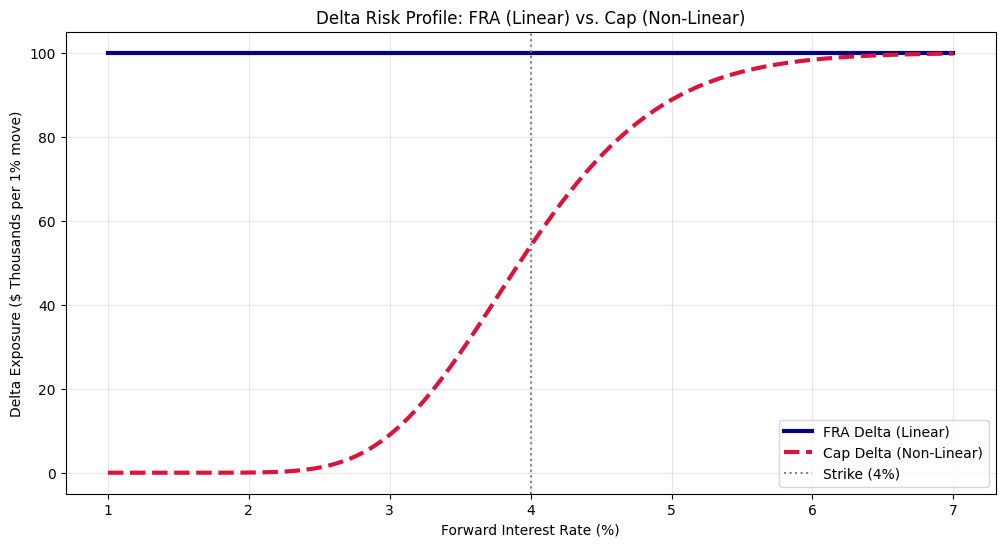
\includegraphics[width=1\linewidth]{images/delta_sensitivity}
		\end{columns}
	\end{itemize}
	
\end{frame}

\begin{frame}{Volatility Sensitivity}
	\begin{itemize}
		\item When we add volatility to the mix, the difference between linear and non-linear portfolios becomes even more dramatic.
		\item While a linear portfolio has a $\Delta$ "blind" to volatility, a non-linear portfolio has a $\Delta$ profile that "warps" whenever market uncertainty changes. %This interaction is known as Vanna (the change in Delta with respect to Volatility).
		\begin{center}
			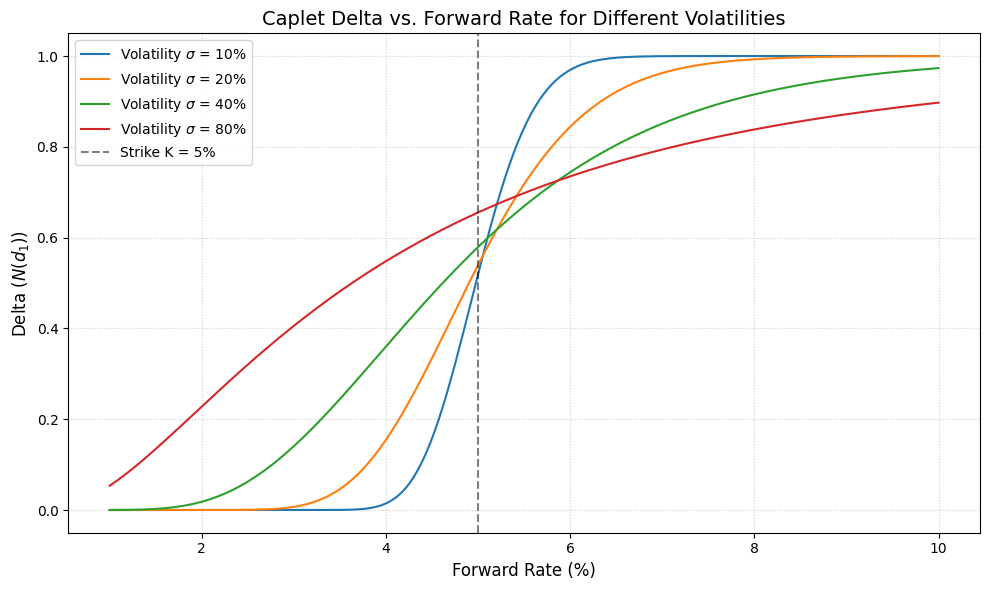
\includegraphics[width=0.5\linewidth]{images/delta_vs_vola}
		\end{center}
		\item The same Cap reacts to interest rates under different volatility regimes. The FRA remains a perfectly flat, its risk is 100\% predictable regardless of volatility.
	\end{itemize}
\end{frame}

\begin{frame}{Vega Sensitivity}
	\begin{itemize}
		\item Vega measures how much the value of your Cap portfolio will change if volatility moves by 1\%.
		\item Unlike $\Delta$, which is highest when the option is deep in-the-money, Vega is highest when the rate is At-The-Money (ATM).
		\item This is because when the rate is exactly at the strike, the "uncertainty" of whether the option will finish in or out of the money is at its peak.
		\begin{center}
			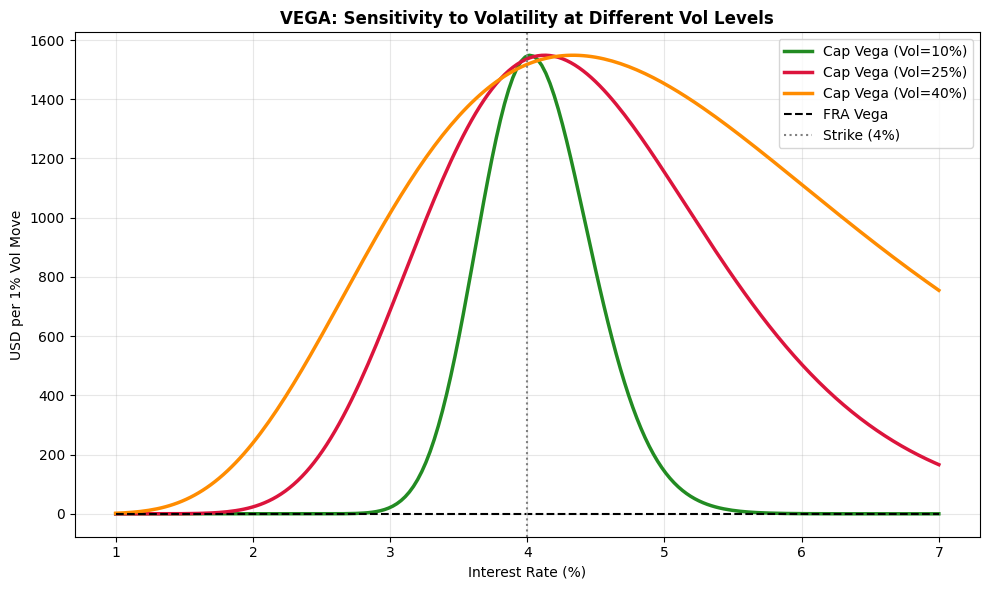
\includegraphics[width=0.5\linewidth]{images/vega_vs_vola}
		\end{center}
	\end{itemize}
\end{frame}

\begin{frame}{Theta ($\Theta$) Sensitivity}
	\begin{itemize}
		\item $\Theta$ refers to the loss of value over time. For a risk manager, though, the more interesting effect is how time changes $\Delta$ profile ("Pinning Risk").
		\item Long Time to Expiry you have $\Delta$ exposure even if the rate is 1\% away from the strike.
		\item As you get closer to expiry, the curve becomes a cliff. If the rate is 3.99\% and the strike is 4.00\%, you have zero $\Delta$. If the rate moves to 4.01\%, you suddenly have 100\% $\Delta$.
		\item This is where traders get "pinned." You have to hedge and re-hedge frantically as the rate dances around the strike in the final hours, because your $\Delta$ is jumping between 0 and 1 (infinite $\Gamma$).
		\begin{center}
			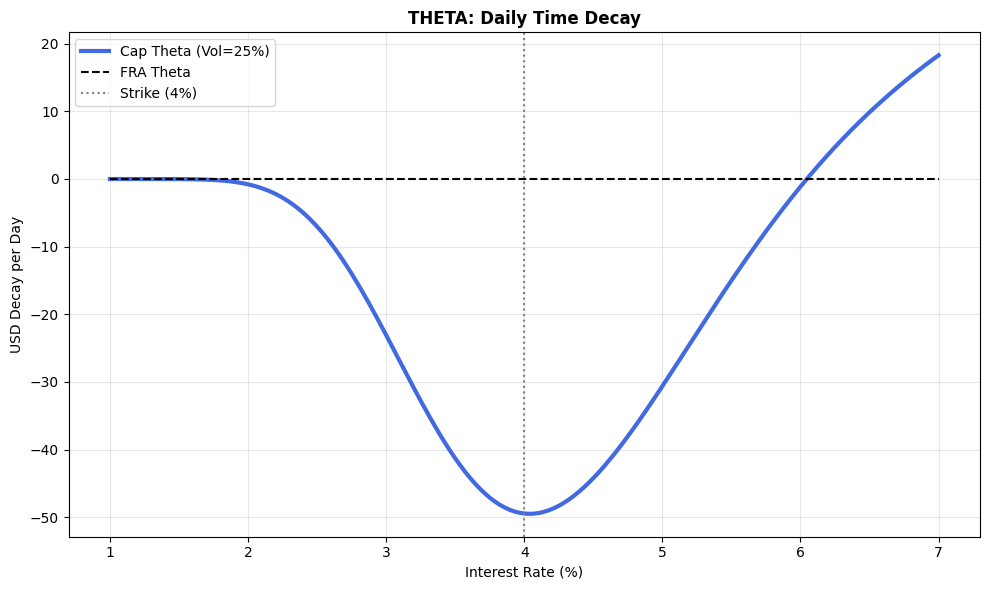
\includegraphics[width=0.45\linewidth]{images/theta}
			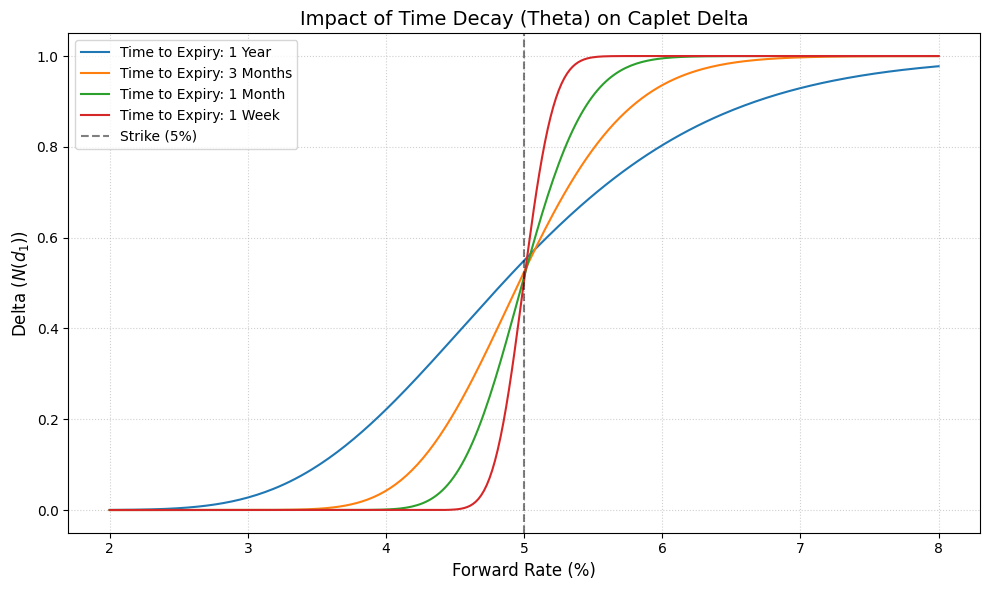
\includegraphics[width=0.45\linewidth]{images/delta_vs_theta}
		\end{center}
	\end{itemize}
\end{frame}

\begin{homework}
	\begin{frame}{\textcolor{white}{Homework}}
		\begin{itemize}
			\item[white] Consider a 2-year Interest Rate Swap on a notional of 1M, with a fixed rate of 5\% and paying Libor rate annually. The term-structure of interest rates is flat at 5\%.
			Estimate the DV01 of the swap numerically.
			\item[white] Calculate the analytical expressions for:
			\begin{itemize}
				\item[white] Delta Sensitivity analytically, that is the first derivative of caplet price w.r.t. the forward rate, using the black model to price a generic caplet;
				\item[white] Delta Vega analytically, that is the first derivative of caplet price w.r.t. the volatility, using the black model to price a generic caplet.
			\end{itemize}
		\end{itemize}
	\end{frame}
\end{homework}

%When moving from linear derivatives (Swaps) to options on those derivatives (Swaptions), calculating the Delta becomes significantly more complex. In a Swaption, the Delta measures the sensitivity of the option price to a change in the underlying swap rate.
%\begin{frame}{The Delta of a Swaption}
%
%	\begin{itemize}
	%		\item Unlike a Swap, where Delta is constant (linear), a Swaption's Delta is non-linear and depends on the "moneyness" of the option.
	%		\item The value of a European Swaption is typically given by the \textbf{Black-76 formula}:
	%		\begin{equation*}
		%			V_{pay} = A_{\alpha,\beta}(t) \left[ S_{\alpha,\beta}(t) \Phi(d_1) - K \Phi(d_2) \right]
		%		\end{equation*}
	%		\item The Delta is the derivative of this price with respect to the forward swap rate S:
	%		\begin{equation*}
		%			\Delta = \frac{\partial V}{\partial S} = A_{\alpha,\beta}(t) \Phi(d_1)
		%		\end{equation*}
	%		\item \textbf{The Complication:} In the market, we often distinguish between:
	%		\begin{itemize}
		%			\item \textbf{Sticky-Strike Delta}: Assumes volatility σ stays constant as the rate moves.
		%			\item \textbf{Sticky-Delta (Shadow Delta)}: Accounts for the \emph{Volatility Smile}. As the rate moves, the implied volatility usually changes (skew), requiring an adjustment: ∂S∂V​+∂σ∂V​∂S∂σ​.
		%		\end{itemize}
	%	\end{itemize}
%\end{frame}

\begin{frame}{Black vs. Stochastic Rates}
	Choosing between the Black-76 formula and a Short Rate model (like Hull-White) depends on the goal of your desk:
	\vfill
	\begin{itemize}
		\item \textbf{Market Standard.} Used for quoting prices and communicating implied volatilities.
		\begin{itemize}
			\item \emph{Use case:} pricing standard vanilla Swaptions in a "flat" vol environment.
			\item \emph{Limitation:} it assumes the swap rate is log-normal; it cannot price path-dependent products.
		\end{itemize}
		\vfill
		\item \textbf{Risk Management \& Exotic Options.} Models like Hull-White ensure the whole yield curve evolves consistently.
		\begin{itemize}
			\item \emph{Use case:} pricing Bermudan Swaptions or managing a portfolio of mixed interest rate products.
			\item \emph{Advantage:} allows for mean reversion and consistent pricing across different tenors.
		\end{itemize}
	\end{itemize}
\end{frame}

\begin{frame}{Swaption Pricing under Affine Models}
	\begin{itemize}
		\item One of the most striking properties of \emph{Affine Models} (e.g. Vasicek, Hull-White) is that the ZCB price is an exponential function of the short rate:
		\begin{equation*}
			P(T_\alpha, T_k) = A(T_\alpha, T_k) e^{-B(T_\alpha, T_k) r(T_\alpha)}
		\end{equation*}
		\item A payer swaption (PSw) value can be calculated as (derivation left as exercise):
		\begin{equation}
			\textbf{PSw} = N\cdot P(t, T_\alpha)\cdot \mathbb{E}^{Q}_t \left[ \left( 1 - \sum_{k=\alpha+1}^\beta c_k P(T_\alpha, T_k) \right)^+ \right]
			\label{eq:swaption_payoff_std_v2}
		\end{equation}
		\item As previously said unfortunately the summation is \emph{inside} the $\max$ operator, so we cannot solve for a "swaplet" object\ldots
		%		\item By Jamshidian's Decomposition, we find $r^*$ such that $\sum c_k P(T_\alpha, T_k, r^*) = 1$.
	\end{itemize}
\end{frame}

\begin{frame}{Jamshidian's Decomposition \colablink{https://colab.research.google.com/drive/1NSytELQY4QciO4zRPGOiRro1FDtnD1N_}}
	\begin{block}{Theorem}
		Consider a sequence of functions $f_i$, a random variable $W$ and a constant $K\ge0$. If each $f_i$ is monotone (decreasing), that is $\cfrac{\partial f_i}{\partial W} < 0;\;\forall i$, then
		\begin{equation*}
			\left(K - \sum_i f_i(W)\right)^+ = \sum_i \left(K_i - f_i(W)\right)^+
		\end{equation*}
		In financial terms it means that the payoff of an option on a portfolio of assets can be expressed in terms of a portfolio of options on each asset.
	\end{block}
\end{frame}

\begin{frame}{Jamshidian's Decomposition Proof}
	\begin{itemize}
		\item<1-> Since each $f_i$ is monotone also $\sum_i f_i$ is decreasing. Hence there is a unique solution $\hat{w}$ to
		\begin{equation*}
			\sum_i f_i(\hat{w}) = K
		\end{equation*}
		\item<2-> Each $f_i$ is decreasing so
		\begin{columns}
			\column{0.7\linewidth}
			\uncover<2->{\begin{equation*}
					\left(K - \sum_i f_i(W)\right)^+ = \left(\sum_i f_i(\hat{w}) -  \sum_i f_i(W)\right)^+ =
			\end{equation*}}
			\uncover<3->{\begin{equation*}
					= \left(\sum_i (f_i(\hat{w}) -  f_i(W))\right)^+= \sum_i (f_i(\hat{w}) - f_i(W))\mathbbm{1}_{W\ge \hat{w}}
			\end{equation*}}
			\uncover<4->{\begin{equation*}
					= \sum_i \left(K_i - f_i(W)\right)^+\quad\qedsymbol
				\end{equation*}
			}
			\column{0.35\linewidth}
			\uncover<1->{
				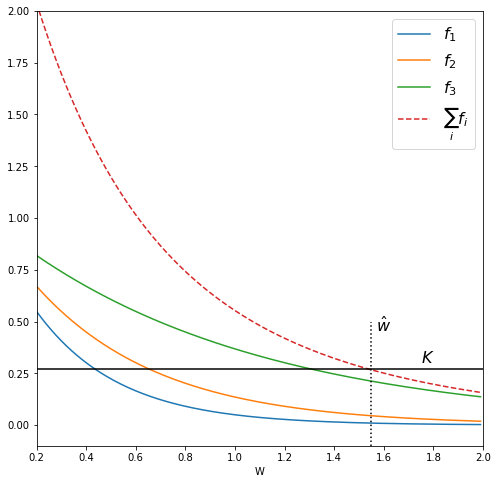
\includegraphics[width=1\linewidth]{images/jamshidian_trick}}
		\end{columns}
	\end{itemize}
\end{frame}

\begin{frame}{Swaption as a Portfolio of ZCB Options \colablink{https://colab.research.google.com/drive/1NSytELQY4QciO4zRPGOiRro1FDtnD1N_}}
	\begin{itemize}
		\item Since each ZCB price is monotone in $r$, the swaption price is the sum of European Put options on the individual Zero-Coupon Bonds:
		\begin{equation}
			\boxed{\textbf{PSw}(t) = N\cdot\sum_{k=\alpha+1}^\beta c_k\cdot \textbf{ZBP}(t, T_\alpha, T_k, X_k)}
		\end{equation}
		where $X_k = P(T_\alpha, T_k, r^*)$ is the strike of the $k$-th ZCB option.
		\item In one-factor affine models, swaptions are not "new" products; they are simply a \textcolor{maincolor}{static portfolio of ZCB options}.
	\end{itemize}
	\vfill
	\begin{block}{Efficiency Note}
		Jamshidian's decomposition is the reason why the Hull-White model is so fast. To calibrate the model to a Swaption, we don't need a Monte Carlo simulation; we just need a sum of Black-Scholes-like formulas for ZCB options.
	\end{block}
\end{frame}

\begin{homework}
	\begin{frame}{\textcolor{white}{Homework}}
		\begin{itemize}
			\item[white] Derive swaption valuation formula as expressed in \cref{eq:swaption_payoff_std_v2}. \textbf{Hint}: start from \cref{eq:swaption_payoff_std}.
		\end{itemize}
	\end{frame}
\end{homework}

%\subsection{Bond Options}
%\begin{frame}{An Option to Exchange Fixed with Float}
%\begin{itemize}
%	\item<1-> We have seen that a Swap can be viewed as an exchange of bonds (fixed for float).
%	\item<2-> Hence a Swaption can be regarded as an \textcolor{red}{option to exchange fixed for floating} bonds (or vice versa).
%	\item<3-> In case it would be possible to get a simple expression for a \textcolor{red}{Coupon Bond Option} we could use to price Swaptions.
%	\item <4-> It would be even simpler if we could express a Coupon Bond Option as a portfolio of Zero Coupon Bond Options.
%	\item<5-> Luckily we can do that thanks to a recipe known as \textcolor{red}{Jamshidian's decomposition}.
%\end{itemize}
%\end{frame}
%
%\begin{frame}{Jamshidian's Decomposition}
%\begin{block}{Theorem}
%	Consider a sequence of functions $f_i$, a random variable $W$ and a constant $K\ge0$. If each $f_i$ is monotone (decreasing), that is $\cfrac{\partial f_i}{\partial W} < 0;\;\forall i$, then
%	\begin{equation*}
	%		\left(K - \sum_i f_i(W)\right)^+ = 	\sum_i \left(K_i - f_i(W)\right)^+
	%	\end{equation*}
%	In financial terms it means that the payoff of an option on a portfolio of assets can be expressed in terms of a portfolio of options on each asset.
%\end{block}
%\end{frame}
%
%\begin{frame}{Jamshidian's Decomposition Proof}
%\begin{itemize}
%	\item<1-> Since each $f_i$ is monotone also $\sum_i f_i$ is decreasing. Hence there is a unique solution $\hat{w}$ to
%	\begin{equation*}
	%		\sum_i f_i(\hat{w}) = K
	%	\end{equation*}
%	\item<2-> Each $f_i$ is decreasing so
%	\begin{columns}
	%		\column{0.7\linewidth}
	%		\uncover<2->{\begin{equation*}
			%				\left(K - \sum_i f_i(W)\right)^+ = \left(\sum_i f_i(\hat{w}) -  \sum_i f_i(W)\right)^+ =
			%		\end{equation*}}
	%		\uncover<3->{\begin{equation*}
			%				= \left(\sum_i (f_i(\hat{w}) -  f_i(W))\right)^+= \sum_i (f_i(\hat{w}) - f_i(W))\mathbbm{1}_{W\ge \hat{w}}
			%		\end{equation*}}
	%		\uncover<4->{\begin{equation*}
			%				= \sum_i \left(K_i - f_i(W)\right)^+\quad\qedsymbol
			%			\end{equation*}
		%		}
	%		\column{0.35\linewidth}
	%		\uncover<1->{
		%			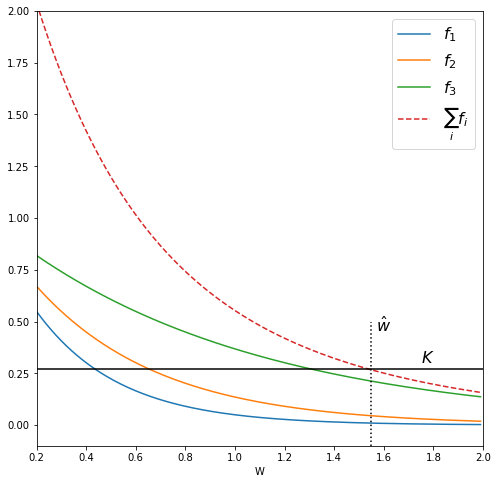
\includegraphics[width=1\linewidth]{images/jamshidian_trick}}
	%	\end{columns}
%\end{itemize}
%\end{frame}
%%Jamshidian's Condition: You correctly identify that fi​ must be monotone. In the context of interest rates, this means the model must be a one-factor model (where the whole curve moves in one direction relative to the short rate r). If you have a two-factor model, Jamshidian’s decomposition generally fails because ZCB prices for different tenors might move in opposite directions.
%
%
%\begin{frame}{Back to Coupon Bond Option}
%\begin{itemize}
%	\item<1-> Consider a coupon bond which pays the following cash flows $\mathcal{C}=\{c_1,\dots,c_n\}$ at dates $\mathcal{T}=\{T_1,\ldots,T_n\}$.
%	\item<2-> Let $t\leq T_1$, the bond price is given by
%	\begin{equation*}
	%		\textbf{CB}(t,\mathcal{C},\mathcal{T})=\sum_{i=1}^n c_i \Pi(t, T_i, r(t))
	%	\end{equation*}
%	\item<3-> Suppose we would like to calculate the price of a put option with strike $K$ on this coupon bond. The payoff reads
%	\begin{equation*}
	%		\textbf{CBP}=\left[K-\textbf{CB}(t,\mathcal{C},\mathcal{T})\right]^+ = \left[K-\sum_{i=1}^n c_i \Pi(t, T_i, r(t))\right]^+
	%	\end{equation*}
%\end{itemize}
%\end{frame}
%
%\begin{frame}{Coupon Bond Option}
%\begin{itemize}
%	\item<1-> Now apply the Jamshidian's decomposition to previous payoff.
%	\item<2-> First need to find the interest rate value $r^*$ such that $\sum_{i=1}^n c_i \Pi(t, T_i, r^*) = K$.
%	\item<3-> Assuming the interest rate model satisfies the required condition (which is true for Short Rate models for example)
%	\begin{equation*}
	%		\frac{\partial \Pi(t,T_i,r(t))}{\partial r}<0,\;\forall 0<t<s
	%	\end{equation*}
%	we can write the payoff as
%	\begin{equation}
	%		\textbf{CBP}(t,T_i,\Pi,r^*) = \sum_{i=1}^n c_i [\Pi(t, T_i, r^*)-\Pi(t, T_i, r(t))]^+
	%		\label{eq:bond_option_payoff}
	%	\end{equation}
%\end{itemize}
%\end{frame}
%
%\begin{frame}{Coupon Bond Option}
%\begin{itemize}
%	\item \cref{eq:bond_option_payoff} tells us that we can price a coupon bond option as a portfolio of options on ZCBs.
%	\item The strike of these option is calculated as the value of a ZCB given a \emph{particular} value of the short rate, determined with a root finding procedure.
%	\item In formulas the CBO with maturity $T$ and strike $K$ reads
%	\begin{equation}
	%		\boxed{\textbf{CBP}(t,\mathcal{T},\mathcal{C},K) = \sum_{i=1}^n c_i \textbf{ZBP}(t,T_i,\Pi,r^*)}
	%	\end{equation}
%\end{itemize}
%\end{frame}
%
%%The Affine Formula: In the slide "Swaption Pricing under Affine Models," you use τk​ inside Ar​ and Br​. Usually, these functions are defined as A(Tα​,Tk​) and B(Tα​,Tk​). Using τk​ might be confused with the year fraction. I recommend keeping the Tα​,Tk​ notation for clarity.
%
%%The Expected Value: You use Et​. Ensure the measure is clear (typically the Tα​-forward measure or the risk-neutral measure with the specific numeraire).
%
%
%\begin{frame}{Swaption Pricing under Affine Models}
%	\begin{itemize}
	%		\item One of the most striking properties of \emph{Affine Models} (Vasicek, Hull-White) is that the ZCB price is an exponential function of the spot rate:
	%		\begin{equation*}
		%			P(T_\alpha, T_k) = A(T_\alpha, T_k) e^{-B(T_\alpha, T_k) r(T_\alpha)}
		%		\end{equation*}
	%		\item A payer swaption (PSw) can be viewed as a Put option on a coupon bond with strike $K_{bond} = 1$:
	%		\begin{equation*}
		%			\textbf{PSw} = N P(t, T_\alpha) \mathbb{E}^{Q^{T_\alpha}}_t \left[ \left( 1 - \sum_{k=\alpha+1}^\beta c_k P(T_\alpha, T_k) \right)^+ \right]
		%		\end{equation*}
	%		\item By Jamshidian's Decomposition, we find $r^*$ such that $\sum c_k P(T_\alpha, T_k, r^*) = 1$.
	%	\end{itemize}
%\end{frame}
%
%\begin{frame}{Final Result: Swaption as a Portfolio of ZCB Options}
%	\begin{itemize}
	%		\item Since each ZCB price is monotone in $r$, the swaption price is the sum of European Put options on the individual Zero-Coupon Bonds:
	%		\begin{equation}
		%			\boxed{\textbf{PSw}(t) = N \sum_{k=\alpha+1}^\beta c_k \textbf{ZBP}(t, T_\alpha, T_k, X_k)}
		%		\end{equation}
	%		where $X_k = P(T_\alpha, T_k, r^*)$ is the strike of the $k$-th ZCB option.
	%		\item \textbf{Conclusion:} In one-factor affine models, swaptions are not "new" products; they are simply a \textcolor{red}{static portfolio of ZCB options}.
	%	\end{itemize}
%\end{frame}
%
%"Jamshidian's decomposition is the reason why the Hull-White model is so fast. To calibrate the model to a Swaption, we don't need a Monte Carlo simulation; we just need a sum of Black-Scholes-like formulas for ZCB options."
%
%
%%\begin{frame}{Swaption Pricing under Affine Models}
%%\begin{itemize}
%%	\item When interest rates are modeled using \textcolor{red}{Affine Short Rate Models} (Vasicek, Hull-White,\ldots) swpation pricing can be performed semi-analytically.
%%	\item \cref{eq:swaption_payoff_std} can be rewritten, expressing the underlying swap in terms of bonds, as
%%	\begin{equation*}
	%%		\textbf{PSw}=NP(t_0, T_\alpha)\mathbb{E}_t\left[\max\left(1-\sum_{k=\alpha+1}^\beta c_kP(T_\alpha,T_k), 0\right)\right]
	%%	\end{equation*}
%%	with $c_k=K\tau_k$ for $k=\alpha+1,\ldots,\beta-1$ and $c_\beta=(1+K\tau_\beta)$.
%%	\item One of the most striking properties of \emph{Affine Models} is that they relate ZCB price to a spot rate modeled according to
%%	\begin{equation*}
	%%		P(t,T) = A_r(t,T)e^{-B_r(t,T)r}
	%%	\end{equation*}
%%\end{itemize}
%%\end{frame}
%%
%%\begin{frame}{Swaption Pricing under Affine Models}
%%\begin{itemize}
%%	\item Hence
%%	\begin{equation*}
	%%		\textbf{PSw}=NP(t_0, T_\alpha)\mathbb{E}_t\left[\max\left(1-\sum_{k=\alpha+1}^\beta c_k A_r(\tau_k)e^{B_r(\tau_k)r(T_\alpha)}, 0\right)\right]
	%%	\end{equation*}
%%	\item Using the Jamshidian decomposition the $\max$ operator can be swapped with the sum
%%	\begin{equation*}
	%%		\textbf{PSw}=NP(t_0, T_\alpha)\sum_{k=\alpha+1}^\beta c_k \mathbb{E}_t\left[\max\left(\bar{K_k} - A_r(\tau_k)e^{B_r(\tau_k)r(T_\alpha)}, 0\right)\right]
	%%	\end{equation*}
%%	whit $\bar{K_k} := A_r(\tau_k)e^{B_r(\tau_k)r^{*}}$, where the parameter $r^{*}$ is determined by solving
%%	\begin{equation*}
	%%		\sum_{k=\alpha+1}^\beta c_k \left(A_r(\tau_k)e^{B_r(\tau_k)r^{*}}\right) = 1
	%%	\end{equation*}
%%\end{itemize}
%%\end{frame}
%%
%%\begin{frame}{Swaption Pricing under Affine Models}
%%\begin{itemize}
%%	\item As noted above for the bond options, each element of the sum in the formula above represents a European put option on a zero-coupon bond, which in the \emph{affine models} has a closed-form solution.
%%	\item So a payer swaption price is thus given by
%%	\begin{equation}
	%%		\boxed{\textbf{PSw}(t,T,N) = N\sum_{k=1}^n c_k \textbf{ZBP}(t,T_k,K_k)}
	%%	\end{equation}
%%	while the receiver swaption price reads
%%	\begin{equation}
	%%		\boxed{\textbf{RSw}(t,T,N) = N\sum_{k=1}^n c_k \textbf{ZBC}(t,T_k,K_k)}
	%%	\end{equation}
%%\end{itemize}
%%\end{frame}
%
%
%
%
%%\begin{frame}{Adapting to Swaptions}
%%\begin{itemize}
%%	\item When interest rates are modeled using \textcolor{red}{Affine Short Rate Models} it is rather simple to arrive to the swaption pricing formula.
%%	\item \emph{Affine Models} indeed relates ZCB price to a spot rate model according to
%%	\begin{equation*}
	%%		P(t,T) = A(t,T)e^{-B(t,T)r}
	%%	\end{equation*}
%%	\item Hence the value $r^*$ can be determined as a solution of
%%	\begin{equation*}
	%%		\sum_{i=1}^n A(t,t_i)e^{-B(t,t_i)r^*}
	%%	\end{equation*}
%%	%%		\item Denote as usual with $\tau_i$ the year fraction between $t_{i-1}$ and $t_i$, fix $c_i=X\tau_i$ and $c_n = 1+X\tau_i$.
%%	%%		\item Let the swap notional be equal to N.
%%	%%		\item Thus for the price of a payer swaption we have to calculate the following payoff
%%	%%		\begin{equation*}
	%%		%%			\left[1-CB(t,\mathcal{C},T)\right]^+
	%%		%%		\end{equation*}
%%	%%		\item We can calculate this payoff via the procedure outlined before.
%%\end{itemize}
%%\end{frame}
%%
%%\begin{frame}{Swaption Pricing via Affine Models}
%%\begin{itemize}
%%	\item Consider an option on a swap which pays a fixed rate $X$ and receives LIBOR.
%%	\item Modeling the short rate with an affine model we can define $r^*$ at time $T$, such that
%%	\begin{equation*}
	%%		\sum_{i=1}^n c_i A(t,T_i)e^{-B(t,T_i)r^*} = 1
	%%	\end{equation*}
%%	where $c_i$ is the coupon value.
%%\end{frame}


\subsection{Bermudan Swaption}
\begin{frame}{Bermudan Swaptions}
	\begin{itemize}
		\item<1-> It is a swaption in which the optionality can be exercised at a \textcolor{maincolor}{predetermined set of dates} (not only one).
		\item<2-> It is useful for hedging callable bonds (especially if step-up, i.e. with the coupon increasing with time).
		\item<3-> A \textcolor{maincolor}{Bermudan Swaption} gives the holder the right but not the obligation to enter in an interest rate swap contract at different dates (usually the swap reset dates) with some days of notification to the counter-party.
		\item<4-> The interest rate swap the holder can enter into, is the same existing contract, so if the holder does not exercise at the first date in the call schedule, the option for the following periods is just written on shorter swaps.
	\end{itemize}
\end{frame}

\begin{frame}{Bermudan Swaption Example}
	\begin{itemize}
		\item<1-> As an example consider the following: receiver Bermudan Swaption written on a 3 years swap with the first call date $2y$ from now (we suppose semi-annual payments).
		\item<2-> If at the end of the second year she will not exercise, six months later she will have to decide if entering or not in the same remaining swap which now has become a $2y6m$ swap.
		\item<3-> If again she will not exercise the last possibility will involve the decision of whether or not to enter on the $2y6m-3y$~$FRA$.
	\end{itemize}
\end{frame}

\begin{frame}{Bermudan Swaption Pricing}
	\begin{itemize}
		\item<1-> Some interest rate instruments can be priced just looking at the term structure of interest rates (FRA and Swaps)
		\begin{itemize}
			\item the only problem is: which is the right term structure ? (this is a lesson from the 2008 crisis).
		\end{itemize}
		\item<2-> Some other instruments cannot be priced only with the yield curve: we need the future (risk-neutral) evolution of the rates.
		\item<3-> Given the complexity of Bermudan swaption valuation (which belongs to the latter class), there is no closed form solution.
		\item<3-> Typically tree techniques or the Longstaff-Schwartz method are used.
	\end{itemize}
\end{frame}

\begin{frame}{Longstaff-Schwartz Algorithm}
	\begin{itemize}
		\item Consider a Bermudan put option with strike $K$ and $n$-years maturity. Each year you can choose whether to exercise or not.
		%Let's implement a MC which actually simulates, besides the evolution of the market, what an investor holding this option would do.
		\item The evolution of the asset value and of the money market account gives
		\begin{equation}
			\begin{gathered}
				S(t_1=1y) = S(t_0)e^{(r-\frac{1}{2}\sigma^2)(t_1-t_0)+\sigma\sqrt{t_1-t_0}\mathcal{N}(0,1)} \\
				B(t_1=1y)=B(t_0)e^{r(t_1-t_0)}
			\end{gathered}
		\end{equation}
		\item At $t_1$ the investor can:
		\begin{itemize}
			\item \textbf{exercise:} in this case we knows exactly the payoff;
			\item \textbf{does not exercise:} the contract has become a European Put Option with shorter maturity.
		\end{itemize}
		\item \emph{At this point how does the investor know if it is convenient to exercise?}
		\item The decision will depend on each choice convenience:
		\begin{equation*}
			\max[K-S_{t_1}, \textbf{Put}(t_1,T;S_{t_1},K)]
		\end{equation*}
		where $\textbf{Put}(t_1,T;S_{t_1},K)$ is the price of the Put (i.e. the \textbf{continuation value}, the value of holding the option instead of early exercising it).
	\end{itemize}
\end{frame}

\begin{frame}{Longstaff-Schwartz Algorithm}
	\begin{itemize}
		\item So the premium of the option is the average of this discounted payoffs calculated in each Monte Carlo simulation
		\begin{equation*}
			\cfrac{1}{N}\sum_i\max[K-S_{t_1}, \textbf{Put}(t_1,T;S_{t_1},K)]
		\end{equation*}
		\item In this case we could price this product because we have an analytical pricing formula for the Put (Black formula), but what if we didn't ?
		\item \textbf{Brute force solution:} for each realization of $S_{t_i}$ we run another Monte Carlo to price the alternative continuation value.
		\item We need to implement nested MC which is usually a very bad idea. Its execution time grows as $N^2$, which becomes prohibitive when you deal with multiple exercise dates !
	\end{itemize}
\end{frame}

\begin{frame}{Longstaff-Schwartz Algorithm}
	Longstaff and Schwarz were looking for a smarter solution analyzing the relationship between the continuation value and the realizations of $S$.
	%We can plot the discounted payoff at maturity, $P_i$ vs $S_i(t_1)$.
	\begin{columns}
		\column{0.5\linewidth}
		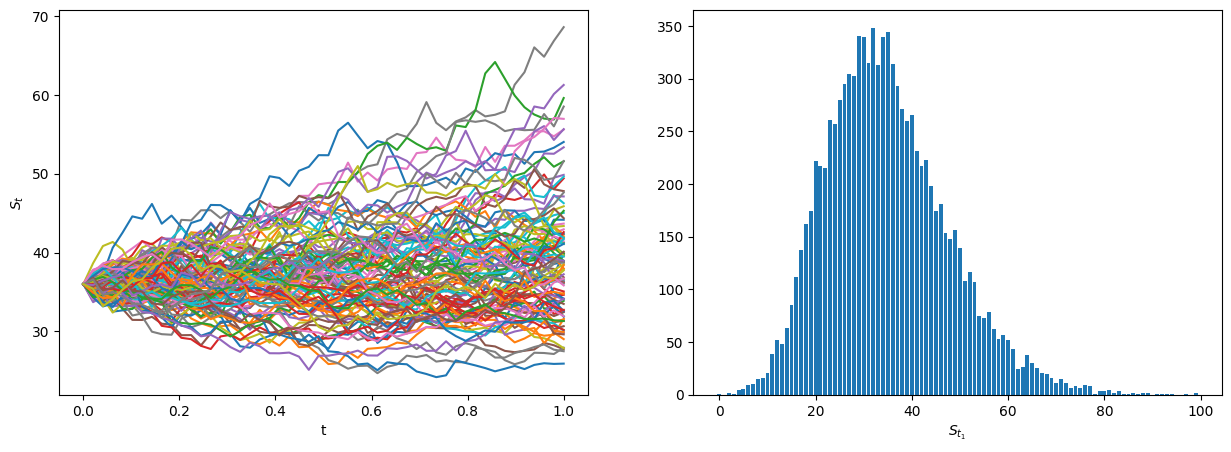
\includegraphics[width=0.9\linewidth]{images/longstaff_simulation}
		
		\small{They found the Put analytical price (green line) was interpolating the cloud of MC points, so \emph{the price at time $t$ can be computed as the barycentre of the discounted payoff cloud.}}
		\column{0.5\linewidth}
		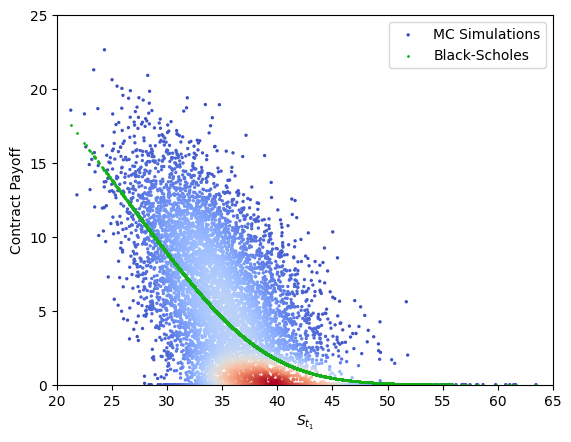
\includegraphics[width=0.9\linewidth]{images/longstaff_scatter_1}
	\end{columns}
	
	\textbf{Estimating the future value of an option $(V)$ can be seen as the problem of finding the curve that best fit the cloud of discounted payoffs at the date of interest.}
\end{frame}

%\begin{frame}{Longstaff-Schwartz Algorithm}
%
%	\begin{itemize}
	%		\item So they found an \emph{empirical pricing formula} for the unknown contract to be used in the Monte Carlo Simulation
	%		\begin{equation}
		%			V(t_i,T,S_{t_i},K)=c_0+c_1 S(t_i) + c_2 S^2(t_i) + c_3 S^3(t_i) + c_4 S^4(t_i) + c_5 S^5(t_i)
		%		\end{equation}
	%		\begin{center}
		%			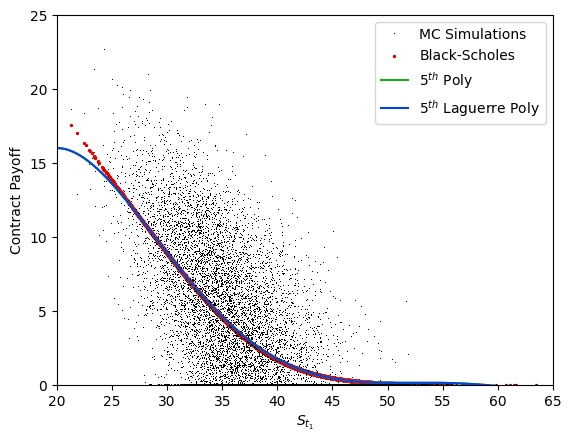
\includegraphics[width=0.35\linewidth]{images/longstaff_scatter_2}
		%		\end{center}
	%		The formula is obviously fast, the cost of the algorithm being just the best fit.
	%		\item Clearly we could have used any form for the curve (not only a polynomial), but the small improvement does not justify the increased complexity.
	%	\end{itemize}
%\end{frame}

\subsection{Callable Bonds}
\begin{frame}{Callable Coupon Bond}
	\begin{itemize}
		\item<1-> A \textcolor{maincolor}{callable bond} is a bond in which, on the call date(s) (there can be more than one), the \textbf{issuer} has the right, but not the obligation, to buy back (redeem) the bonds from the bond holders at a defined call price.
		\item<2-> We have seen that a swap can be regarded as an exchange of bonds. It is easy to guess that a replica for the callable bond price can be obtained by simply adding a (swap-)option to the swap used to price the underlying bond.
		\item<3-> If there are multiple callability dates is clear that we need a \textbf{Bermudan} swaption.
		\item<3-> With a receiver bermudan swaption with the same contractual conventions of the bond (i.e. the strike of the swaption is equal to the coupon of the bond) we can offset it. %; which represents the economic equivalent of calling the bond at par.
		%\item So $\max(CCBP(T,S,K,\tau)-100, 0)$ can be represented as $\max(K-S(T_j,\beta)(T), 0)$.
		%\item Intuition: long on the bond, short on the rates.
	\end{itemize}
\end{frame}

\begin{frame}{Callable vs Non Callable Coupon Bonds}
	\begin{itemize}
		\item<1-> \emph{Ceteris paribus} a non callable coupon bond has an higher price than a callable one because the callability option adds value to the issuer
		\begin{equation*}
			\text{price of callable bond} = \text{price of straight bond} – \text{price of call option}.
		\end{equation*}
		\item<2-> If interest rates decline, the issuer of a callable bond can issue new debt, at lower interest rate than the original one, and use the the proceeds from this second issue to pay off the earlier callable bond by exercising the call feature.
		\item<2-> As a result, \textcolor{maincolor}{the company has refinanced its debt by paying off the higher-yielding callable bonds with the newly-issued debt at a lower interest rate}.
		%	\item At inception both must be worth 100 (apart from other costs and fees which we will neglect).
		%	\item A typical coupon bond, once credit risk is isolated and remunerated, will pay the average market rates prevailing at the time of the issue. These are related to the swap rate prevailing at that moment (remember that the swap rate is sort of average of forward rates).
	\end{itemize}
\end{frame}

%\begin{frame}{Callable vs Non Callable Coupon Bonds}
%\begin{itemize}
%	\item Suppose credit risk is zero: in this ideal case the coupon bond will pay the corresponding swap rate prevailing on the market.
%	If we price a $5y$ bond, at inception, the following must hold
%	\begin{equation*}
	%		CBP(0,5,K,\tau)=100-NPV_{\text5y-swap(0)}=100
	%	\end{equation*}
%	\item Which implies $NPV_{\text{5y-swap(0)}}=0$, hence $K=S_{\text{5y-swap(0)}}$. This means that credit consideration apart, a bank must pay the market prevailing rate when it issues a bond. %And this should not surprise anyone.
%\end{itemize}
%\end{frame}

%\begin{frame}{Callable vs Non Callable Coupon Bonds}
%\begin{itemize}
%	\item Consider now the same bond with a callability option after two years each six months.
%	\item Let us denote with $RBS(t,6m,T_{1c},T_\beta,K,N)$ the Bermudan receiver swaption with first call date $T_{1c}$ and subsequent ones every six months. The last payment date is equal to the swap maturity.
%	\item In this case the call dates vector is $[2y,2y6m,3y,3y6m,4y,4y6m]$.
%	\item Suppose $RBS(0,6m,T_{2y},T_{5y},K_1,N)>0$
%	\begin{equation*}
	%		CBP(0,5,K,\tau)=100-(NPV_{\text{5y-swap(0)}}+NPV_{RBS})=100
	%	\end{equation*}
%\end{itemize}
%\end{frame}

\begin{frame}{Risk Analysis of Callable Bonds}
	\begin{itemize}
		\item A callable bond benefits the issuer, and so investors of these bonds are compensated with a more attractive interest rate than on otherwise similar non-callable bonds.
		%\item Paying down debt early by exercising callable bonds saves a company interest expense and prevents the company from being put in financial difficulties in the long term if economic or financial conditions worsen.
		\item<1-> The investor might not make out as well as the company when rates decrease and the bond is called. Not only she loses the remaining interest payments but unlikely she will be able to match the original coupon.
		\textcolor{maincolor}{This situation is known as reinvestment risk}.
		
		%For example, let's say a 6\% coupon bond is issued and is due to mature in five years. An investor purchases 10000 worth and receives coupon payments of 6\% x 10,000 or 600 annually. Three years after issuance, the interest rates fall to 4\%, and the issuer calls the bond. The bondholder must turn in the bond to get back the principal, and no further interest is paid.
		%In this scenario, not only does the bondholder lose the remaining interest payments but it would be unlikely they will be able to match the original 6\% coupon.
		\item<2-> As a result, a callable bond may not be appropriate for investors seeking stable income and predictable returns.
	\end{itemize}
\end{frame}

\begin{frame}{Break-even Rate}
	\begin{itemize}
		\item<1-> In general, we can assume that \textbf{it is optimal for the issuer to minimize the market value of the callable bond} (how much is worth today for the issuer to settle the debt).
		\item<2-> Imagine a callable bond with a 5\% coupon. If market rates rise to 10\%, the 5\% bond looks "bad" to investors, so its MV drops. The issuer is happy because the debt is now "cheap" to buy back in the open market.
		\begin{itemize}
			\item<3-> If rates stay high, the bond value stays low; the issuer does nothing.
			\item<3-> If rates fall, the bond value tries to climb. The issuer minimizes that climb by exercising the call option when the callable bond exceeds the exercise price ($X$) at the notice date ($t_n$).
			\item<3-> Otherwise, she will give up the option right and the callable bond price will be equal to a non-option bond.
		\end{itemize}
		\item<4-> Denote by $r_b$ the \emph{break-even interest rate} which represents the rate value such that the issuer is indifferent between exercising the option or not.
		\begin{equation}
			X\cdot D(t_n, t_c) - P(r,t_n)=0
		\end{equation}
		where $D(t_n, t_c)$ is the discount factor and $P(r,t_n)$ (callable bond price just before the notice date) is equal to the non-option bond value.
	\end{itemize}
	%We know the value of the callable bond $P(r,t_n)$ since it is equal to the value of the non-option bond. The solution of equation is the cross point between the two curves.
\end{frame}

\begin{frame}{Break-even Rate}
	\textbf{The solution is the cross point between the two curves.}
	\begin{center}
		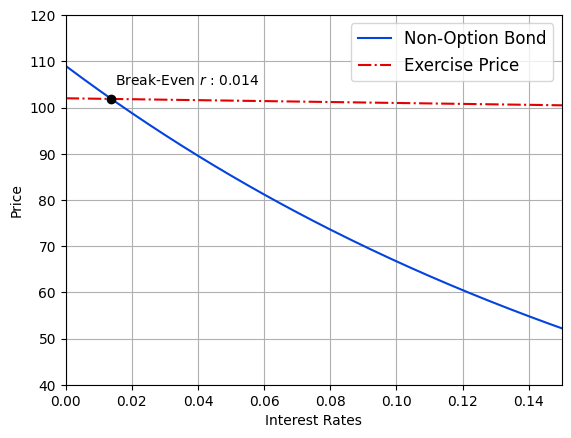
\includegraphics[width=0.5\linewidth]{images/callable_bond}
	\end{center}
\end{frame}

\begin{homework}
	\begin{frame}{\textcolor{white}{Homework}}
		\begin{itemize}
			\item[white] A pension fund holds a 3-year Bermuda Receiver Swaption on a 100 million notional. The strike rate is $K=4\%$.
			The swaption allows the holder to enter a receiver swap (receive fixed, pay floating) at $T=1$ or $T=2$. If exercised, the swap lasts until the final maturity at $T=3$.
			
			Current time is $T=0$. At $T=1$, the 2-year Swap Rate is predicted to be either 3\% or 5\% (50/50 probability). At $T=2$, the 1-year Swap Rate is predicted to be either 2\% or 6\%.
			Assume a flat discount rate of $r=4\%$ for all NPV calculations.
			
			\begin{itemize}
				\item[white] If the holder exercises at $T=1$, what is the tenor of the resulting swap ?
				\item[white] What if they exercise at $T=2$ ?
				\item[white] Calculate the payoff at $T=1$ if the market swap rate is 3\%.
				\item[white] At $T=1$, if the market rate is 3\%, the holder sees an immediate payoff but also knows there is a chance the rate drops to 2\% at $T=2$. Explain qualitatively why the holder might wait instead of exercising at $T=1$.
			\end{itemize}
			\item[white] An investor is looking at a 3-year Callable Bond with a 5\% annual coupon and a par value of 100. The bond is "Callable at Par" (100) at the end of Year 1 and Year 2.
			\begin{itemize}
				\item[white] Scenario A (Falling Rates): At $T=1$, the market yield for a 2-year bond drops to 3\%.
				\item[white] Scenario B (Rising Rates): At $T=1$, the market yield for a 2-year bond rises to 7\%.
			\end{itemize}
			
		\end{itemize}
	\end{frame}
\end{homework}


\section{Change of Measure}
\subsection{Numeraires}
\begin{frame}{Numeraires}
	\begin{itemize}
		\item<1-> Since the main issue in pricing theory is to compute
		\begin{equation}
			\Pi_t = \E^{\mathbb{Q}^X}\left[\frac{1}{X_T}V_A|\mathcal{F}_t\right]
			\label{eq:risk_neutral_pricing}
		\end{equation}
		ideally we would like to define a probability measure $\mathbb{Q}^X$ under which the discounted derivative process is a martingale and such that the expectation of the payoff is analytically tractable (i.e. easy to compute).
		\item<1-> We can determine such measure $\mathbb{Q}^X$ with a \textcolor{maincolor}{change of numeraire}.
		\item<2-> A \textcolor{maincolor}{numeraire} is any strictly positive stochastic process $N_t$ that is taken as unit of reference when pricing an asset $S_t$
		\begin{equation*}
			\tilde{S_t}:=\frac{S_t}{N_t}, \quad t \ge 0
		\end{equation*}
	\end{itemize}
\end{frame}

\begin{frame}{How to Choose a Numeraire}
	\begin{itemize}
		\item We may compute asset values w.r.t. USD, EUR or JPY. Others might prefer commodities: 1~oz of gold could be a numeraire.
		\item In any case, once we choose a numeraire, all the other asset values are determined.
		\item Practical reasons induce to prefer one numeraire to others but theory doesn't suggest there is a best one. \textbf{We want to exploit this in our financial models.}
		\begin{columns}
			\column{0.5\linewidth}
			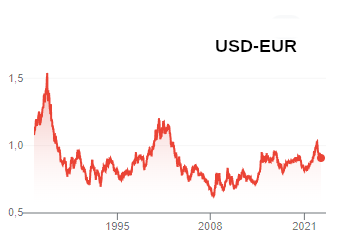
\includegraphics[width=0.9\linewidth]{images/usd_eur}
			\column{0.5\linewidth}
			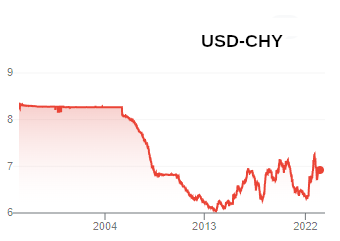
\includegraphics[width=0.9\linewidth]{images/usd_chy}
		\end{columns}
	\end{itemize}
\end{frame}

\begin{frame}{Deterministic or Stochastic Numeraires}
	\begin{itemize}
		\item<1-> \textcolor{maincolor}{Deterministic numeraires} are easy to handle as they imply just an algebraic transformation (i.e. do not involve any risk),
		\begin{itemize}
			\item the exchange rate of the Italian Lira to the Euro was locked at EUR 1 = ITL 1936.27 on 31 December 1998.
		\end{itemize}
		\item<2-> When the numeraire is a \textcolor{maincolor}{stochastic process}, and we want to move to it, the pricing of a claim has to be changed in order to take into account the new risk (the intrinsic randomness of the new numeraire).
		\item<3-> In particular a change of numeraire implies also a change in the underlying measure (probability distribution). Indeed, starting with the bank account numeraire
		\begin{equation*}
			\begin{cases}
				\cfrac{S}{B_t} = \cfrac{\sum_i S_i p_i}{e^{rt}}\\
				\cfrac{U}{B_t} = \cfrac{\sum_i U_i p_i}{e^{rt}}
			\end{cases}\implies
			\frac{S}{U} = \frac{\sum_i S_i p_i}{\sum_j U_j p_j} = \sum_i S_i \frac{p_i}{\sum_j U_j p_j} = \sum_i S_i \pi_i
		\end{equation*}
	\end{itemize}
\end{frame}

\begin{frame}{Stochastic Numeraire Examples (I)}
	\begin{itemize}
		\item<1-> \textbf{Money market account.} Given $r_t$, a possibly random and time dependent risk-free interest rate process, let
		\begin{equation*}
			B_t := \exp\left(\int_0^t r_s ds\right)
		\end{equation*}
		In this case
		\begin{equation*}
			\tilde{S_t}:=\frac{S_t}{B_t}=e^{-\int_0^t r_s ds}S_t, \quad t \ge 0
		\end{equation*}
		represents the discounted price of the asset at time 0.
		\item<2-> \textbf{Currency exchange rate.} In this case $N_t := R_t$ denotes e.g. the EUR/SGD exchange rate. Let
		\begin{equation*}
			\tilde{S_t}:=\frac{S_t}{R_t}, \quad t \ge 0
		\end{equation*}
		denotes the price of a local (SG) asset quoted in units of the foreign currency (EUR) (notice the difference with previous ITL/EUR example above).
	\end{itemize}
\end{frame}

\begin{frame}{Stochastic Numeraire Examples (II)}
	\begin{itemize}
		\item<1-> \textbf{Forward numeraire.} The price $P(t,T)$ of a bond paying $P(T,T)=1$ at maturity $T$. In this case
		\begin{equation*}
			N_t := P(t,T)=\E\left[e^{\int_t^T r_s ds}\right]
		\end{equation*}
		%Notice that the process $t\rightarrow e^{\int_0^t r_s ds} P(t,T)=\E\left[e^{\int_0^T r_s ds}\right], \quad 0 \le t \le T$ is a martingale.
		\item<2-> \textbf{Annuity numeraire.} Processes of the form
		\begin{equation*}
			N_t = P(t, T_0, T_n) := \sum_{k=1}^{n}(T_k - T_{k-1})P(t, T_k), \quad 0 \le t \le T
		\end{equation*}
		where $P(t,T_1),P(t,T_2),\ldots,P(t,T_n)$ are bond prices with maturities $T_1 < T_2 < \ldots < T_n$.
	\end{itemize}
\end{frame}

\subsection{Radon-Nikodym Derivative}
\begin{frame}{Radon-Nikodym Derivative}
	We need to understand how to pass from a numeraire to another, hence by a measure to another, in an arbitrage free setting (until now we have worked with the bank account $B$ numeraire).
	\begin{block}{Definition}
		When two measures are equivalent it is possible to express the first in terms of the second through the \textcolor{maincolor}{Radon-Nikodym derivative}. Indeed there exists a strictly positive \textcolor{maincolor}{martingale process $\zeta_t$} such that
		\begin{equation*}
			\mathbb{Q}^* =\int_{A} \zeta_t(\omega)d\mathbb{Q}(\omega) := \frac{d\mathbb{Q}^*}{d\mathbb{Q}} = \zeta_t
			\label{eq:radon_nikodym_der}
		\end{equation*}
	\end{block}
\end{frame}

\begin{frame}{Intuition from Expected Value}
	\begin{itemize}
		\item To get a sense about Radon-Nikodym derivative, consider a function $F(x)$ with density function $p(x)$ under a measure $\mathbb{P}$.
		\item Suppose there exists a function $q(x)$, which the properties of a density function, then we can write
		\begin{equation*}
			\expect{P}[F(x)]=\int F(x)p(x)dx = \int F(x)p(x)\frac{q(x)}{q(x)}dx
		\end{equation*}
		\item If we define $\psi(x)=F(x)\frac{p(x)}{q(x)}$ the expected value can be written as
		\begin{equation*}
			\expect{P}[F(x)] =\int\psi(x)q(x)dx=\expect{Q}[\psi(x)]=\expect{Q}\left[F(x)\frac{p(x)}{q(x)}\right]
			=\expect{Q}\left[F(x)\zeta\right]
		\end{equation*}
		\item The process $\zeta$ tracks the \emph{likelihood ratio} between two measures and transforms the expectations dynamically. What is $\E[\zeta]$ ? Intuitively, we have that
		\begin{equation*}
			\E^\mathbb{Q}[\zeta]=\E^\mathbb{Q}\left[\frac{d\mathbb{P}}{d\mathbb{Q}}\right]=\int \frac{p(x)}{\cancel{q(x)}} \cancel{q(x)} dx =\int p(x)dx = 1
		\end{equation*}
	\end{itemize}
	
\end{frame}

\begin{frame}{Conditional Expectations}
	\begin{itemize}
		\item In case of a conditioned expectation
		\begin{equation}
			\expect{P}[X|\mathcal{F}_t] = \frac{\expect{Q}\left[X\cfrac{d\mathbb{P}}{d\mathbb{Q}}\bigg|\mathcal{F}_t\right]}{\expect{Q}[\zeta_t|\mathcal{F}_t]}
			\label{eq:conditioned_expectation}
		\end{equation}
		\item To prove this result, for $A \in \mathcal{F}_t$:
		\begin{align*}
			\int_A \frac{\mathbb{E}^\mathbb{Q}[X\zeta_T|\mathcal{F}_t]}{\zeta_t} d\mathbb{P} &= \int_A \frac{\mathbb{E}^\mathbb{Q}[X\zeta_T|\mathcal{F}_t]}{\zeta_t} \zeta_T d\mathbb{Q} = \quad \text{by tower property}  \\
			&= \int_A \mathbb{E}^\mathbb{Q} \left[ \frac{\mathbb{E}^\mathbb{Q}[X\zeta_T|\mathcal{F}_t]}{\zeta_t} \zeta_T \bigg| \mathcal{F}_t \right] d\mathbb{Q} = \int_A \frac{\mathbb{E}^\mathbb{Q}[X\zeta_T|\mathcal{F}_t]}{\zeta_t} \mathbb{E}^\mathbb{Q}[\zeta_T|\mathcal{F}_t] d\mathbb{Q} \\
			&= \int_A \mathbb{E}^\mathbb{Q}[X\zeta_T|\mathcal{F}_t] d\mathbb{Q} = \int_A X\zeta_T d\mathbb{Q} = \int_A X d\mathbb{P}
		\end{align*}
	\end{itemize}
\end{frame}

\begin{frame}[fragile]{Radon-Nikodym Derivative Example \colablink{https://colab.research.google.com/drive/1BDwV4VnNoRE28eGXxwEUnRbIjmL8XZSZ}}
	\begin{itemize}
		\item Imagine two probability densities $\mathbb{P} = \mathcal{N}(\mu_1, \sigma_1)$ and $\mathbb{Q} = \mathcal{N}(\mu_2, \sigma_2)$.
		\item Let's numerically compute the Radon-Nikodym derivative that moves you from the $\mathbb{P}$ to the $\mathbb{Q}$ world.
	\end{itemize}
	\begin{center}
		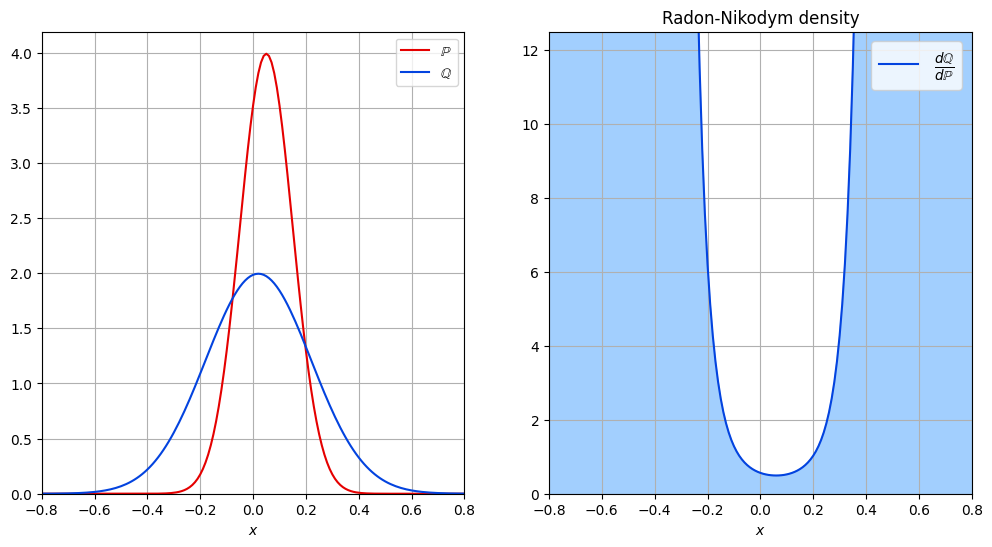
\includegraphics[width=0.75\linewidth]{images/radon_nikodym_plot}
	\end{center}
\end{frame}

\begin{frame}{Importance Sampling Technique \colablink{https://colab.research.google.com/drive/1BDwV4VnNoRE28eGXxwEUnRbIjmL8XZSZ}}
	\begin{itemize}
		\item The Radon-Nikodym derivative serves as the mathematical "bridge" that makes \emph{Importance Sampling} possible.
		\item In Importance Sampling, we calculate an expectation by drawing samples from a "distorted" distribution—one that makes rare events happen more frequently—rather than the original distribution.
		\item Because we have changed the probabilities of these events, our raw results are biased. \item The Radon-Nikodym derivative acts as a corrective weight for each sample; it measures the relative likelihood of a value occurring under the original measure versus the new one.
		\item By multiplying our simulated outcomes by this derivative, we effectively "undo" the distortion, ensuring our final estimate is an unbiased representation of the original system.
	\end{itemize}
\end{frame}

\subsection{Change of Numeraire}
\begin{frame}{Change of Numeraire}
	\begin{block}{Theorem}
		Assume exists a numeraire $N_t$ and the associated measure $\mathbb{Q}^N$, \textit{equivalent} to $\mathbb{P}$, such that the price of every traded asset $S_t$ relative to $N$ is a \textit{martingale} under $\mathbb{Q}^N$.
		\begin{enumerate}
			\item Let $U$ be another arbitrary numeraire, \textbf{there exists a measure $\mathbb{Q}^U$, also equivalent to $\mathbb{P}$, such that the price of every traded asset $S_t$, normalized to $U$, is a martingale under $\mathbb{Q}^U$}
			\begin{equation*}
				\frac{S_t}{U_t} = \expect{U}\left[\frac{S_T}{U_T}\bigg|\mathcal{F}_t\right],\quad 0\le t \le T
			\end{equation*}
			\item The Radon-Nikodym derivative defining the measure $\mathbb{Q}^U$ is given by
			\begin{equation}
				\frac{d\mathbb{Q}^U}{d\mathbb{Q}^N} = \frac{U_T N_t}{U_t N_T}
				\label{eq:radon_nikodym_der2}
			\end{equation}
		\end{enumerate}
	\end{block}
\end{frame}

\begin{frame}{Change of Numeraire (Proof part 2)}
	\begin{itemize}
		\item Let's prove first the second part.
		\item By definition of $\mathbb{Q}^N$, for every asset price $S_t$ holds
		\begin{equation*}
			\begin{cases}
				\cfrac{S_t}{N_t} = \expectt{N}{t}\left[\cfrac{S_T}{N_T}\right] \\
				\expectt{U}{t}\left[\cfrac{S_T}{N_T}\cfrac{d\mathbb{Q}^N}{d\mathbb{Q}^U}\right] = \cfrac{S_t}{N_t} = \cfrac{U_t S_t}{N_t U_t}
				= \cfrac{U_t}{N_t}\expectt{U}{t}\left[\cfrac{S_T}{U_T}\right] = \expectt{U}{t}\left[\cfrac{U_t S_T}{N_t U_T}\right]
			\end{cases}
		\end{equation*}
		\item Since both equations result in $S_t/N_t$ they can be equated
		\begin{equation*}
			\expectt{N}{t}\left[\cfrac{S_T}{N_T}\right] = \expectt{U}{t}\left[\cfrac{U_t S_T}{N_t U_T}\right]
		\end{equation*}
	\end{itemize}
	\vfill
	\begin{tcolorbox}[colback=gray!5, colframe=maincolor, arc=0mm, boxrule=0.5pt]
		\footnotesize
		From time to time to ease the notation I will use $\expect{N}\left[\cdots \middle| \mathcal{F}_t\right] = \expectt{N}{t}\left[\cdots\right]$
	\end{tcolorbox}
\end{frame}

\begin{frame}{Change of Numeraire (Proof part 2)}
	\begin{itemize}
		\item By definition of Radon-Nikodym derivative and from the result of the previous slide, it holds
		\begin{equation*}
			\begin{cases}
				\expectt{N}{t}\left[\cfrac{S_T}{N_T}\right] =\expectt{U}{t}\left[\cfrac{S_T}{N_T} \cfrac{d\mathbb{Q}^N}{d\mathbb{Q}^U}\right] \\
				\expectt{N}{t}\left[\cfrac{S_T}{N_T}\right] =\expectt{U}{t}\left[\cfrac{U_t S_T}{N_t U_T}\right]
			\end{cases}\implies
			\cfrac{\cancel{S_T}}{N_T} \cfrac{d\mathbb{Q}^N}{d\mathbb{Q}^U} = \cfrac{U_t \cancel{S_T}}{N_t U_T}
		\end{equation*}
		where we have used the fact that the expectation arguments under $U$ must equal to get \cref{eq:radon_nikodym_der2}.
	\end{itemize}
	\myendproof
\end{frame}

\begin{frame}{Change of Numeraire (Proof part 1)}
	\begin{itemize}
		\item The conditional expectation under the new measure $\mathbb{Q}^U$ is:
		\begin{equation*}
			\mathbb{E}^U \left[ \frac{S_T}{U_T} \bigg| \mathcal{F}_t \right] = \frac{\mathbb{E}^N \left[ \frac{d\mathbb{Q}^U}{d\mathbb{Q}^N} \frac{S_T}{U_T} \bigg| \mathcal{F}_t \right]}{\mathbb{E}^N \left[ \frac{d\mathbb{Q}^U}{d\mathbb{Q}^N} \bigg| \mathcal{F}_t \right]}
		\end{equation*}
		\item Substituting the Radon-Nikodym derivative $\frac{d\mathbb{Q}^U}{d\mathbb{Q}^N} = \frac{U_T / U_0}{N_T / N_0}$:
		\begin{align*}
			\text{Numerator:} \quad & \mathbb{E}^N \left[ \frac{U_T N_0}{U_0 N_T} \frac{S_T}{U_T} \bigg| \mathcal{F}_t \right] = \frac{N_0}{U_0} \mathbb{E}^N \left[ \frac{S_T}{N_T} \bigg| \mathcal{F}_t \right] = \frac{N_0 S_t}{U_0 N_t} \\
			\text{Denominator:} \quad & \mathbb{E}^N \left[ \frac{U_T N_0}{U_0 N_T} \bigg| \mathcal{F}_t \right] = \frac{N_0}{U_0} \mathbb{E}^N \left[ \frac{U_T}{N_T} \bigg| \mathcal{F}_t \right] = \frac{N_0 U_t}{U_0 N_t}
		\end{align*}
		\item The ratio yields $\frac{S_t}{U_t}$, proving the martingale property.
	\end{itemize}
	\myendproof
\end{frame}

\begin{frame}{Change of Numeraire Remarks}
	This powerful theorem, we have just proved allows to
	\begin{enumerate}
		\item give a simple rule to write (the otherwise difficult to derive) Radon-Nikodym derivative;
		\item the arbitrage-free price of a claim $V$ at time $t$ is unique. The choice of numeraire only changes the \textit{representation} of the calculation:
		\begin{equation*}
			V_t = B_t \mathbb{E}^{B} \left[ \frac{V_T}{B_T} \bigg| \mathcal{F}_t \right] = N_t \mathbb{E}^{N} \left[ \frac{V_T}{N_T} \bigg| \mathcal{F}_t \right]
		\end{equation*}
		\item find an easier expression of our process to work-out the pricing formula. It is often algebraically more tedious under the risk-neutral measure $V_t=\mathbb{E}^{B}[e^{-r(T-T)}\text{Payoff}(S_T)|\mathcal{F}_t]$.
		The "difficulty" arises dealing with the discount factor inside or outside the expectation.
		By switching to measure $\mathbb{Q}^N$:
		\begin{itemize}
			\item "normalize" the world so that $N$ is the benchmark.
			\item the relative price $S/N$ is a \textcolor{maincolor}{driftless process}.
			\item the discount factor often is "absorbed" by the RND.
		\end{itemize}
	\end{enumerate}
\end{frame}


%	\begin{frame}{Asset Price divided by Numeraire}
	%		\begin{itemize}
		%			\item<1-> Let $B$ be the money market account and $\mathbb{Q}^B$ the corresponding risk-neutral measure. Also let $N$ be another numeraire (note that for what just said $N/B$ is a $\mathbb{Q}^B$-martingale).
		%			\item<2-> From the Change of Numeraire Theorem we can define a new measure by mean of
		%			\begin{equation*}
			%				\frac{d\mathbb{Q}^N}{d\mathbb{Q}^B} = \frac{N_TB_0}{B_TN_0}
			%			\end{equation*}
		%			\item<3-> Then, for any asset $S$ such that $S/B$ is a $\mathbb{Q}^B$-martingale
		%			\begin{equation*}
			%				\expect{N}\left[\frac{S_T}{N_T}\bigg|\mathcal{F}_t\right] = \cfrac{\expect{B}\left[\cfrac{S_T}{N_T}\cfrac{N_TB_0}{B_TN_0}\bigg|\mathcal{F}_t\right]}{\expect{B}\left[\cfrac{N_TB_0}{B_TN_0}\bigg|\mathcal{F}_t\right]}
			%				=\cfrac{\expect{B}\left[\cfrac{S_T}{B_T}\bigg|\mathcal{F}_t\right]}
			%				{\expect{B}\left[\cfrac{N_T}{B_T}\bigg|\mathcal{F}_t\right]}
			%				=\frac{S_tB_t}{N_tB_t}=\frac{S_t}{N_t}
			%			\end{equation*}
		%			\myendproof
		%			\item<4-> \textcolor{maincolor}{So $S/N$ is a $\mathbb{Q}^N$-martingale.}
		%		\end{itemize}
	%	\end{frame}

\subsection{Applications}
\begin{frame}{$S/N$ as Driftless Process}
	\footnotesize{\tiny {\tiny }}{
		\begin{table}[bt]
			\renewcommand*{\arraystretch}{1.4}
			\begin{tabular}{|l|l|} \hline
				\begin{tabular}{@{}l@{}}
					Any asset divided by the bank account
					$B_t$\\(recall $dB_t = r_t B_t dt$)
					\boxed{\cfrac{S_t}{B_t} = e^{-\int_0^t r_s ds}S_t}
				\end{tabular}
				& \begin{tabular}{l}
					It is a martingale under the\\
					measure $\mathbb{Q}^B$ associated to \\
					the bank account numeraire,\\
					i.e. the risk neutral measure.
				\end{tabular} \\ \hline
				\begin{tabular}{@{}l@{}}
					The forward rate\\
					\boxed{F(t; T_1, T_2) = \frac{1}{T_2-T_1}\left(\frac{P(t,T_1) - P(t,T_2)}{P(t,T_2)}\right)}\\
					can be interpreted as a portfolio of two ZCBs\\
					divided by another ZCB.
				\end{tabular}
				& \begin{tabular}{l}
					Under the measure $\mathbb{Q}^{T^2}$\\
					associated to the numeraire\\
					$P(\cdot,T_2)$ it is a martingale.\end{tabular}\\ \hline
				\begin{tabular}{@{}l@{}}
					The swap rate
					\boxed{S_{\alpha,\beta}(t) = \frac{P(t,T_\alpha)-P(t,T_\beta)}{\sum_{i=\alpha+1}^{\beta}\tau_i P(t,T_i)}}
					\\can be interpreted as a portfolio of two ZCBs\\
					divided by a portfolio of ZCBs.
				\end{tabular}
				& \begin{tabular}{l}
					It is a martingale under the\\
					measure associated to the\\
					annuity numeraire.
				\end{tabular} \\ \hline
			\end{tabular}
	\end{table}}
\end{frame}

%	\begin{frame}{A Useful Separation}
	%		\begin{itemize}
		%			\item<1-> Until now we have used $B(t)$, the money market account, as numeraire. But as we have seen it is natural to look for the most convenient one, that is, the one which minimizes the mathematical difficulties according to the problem at hand.
		%			\item<2-> Given a contingent claim whose payoff at time $T$ is $\chi$, we have the following formula for its price $\Pi$
		%			\begin{equation*}
			%				\Pi_\chi(t,T)=\expect{B}\left[e^{-\int_t^T r_s ds}\chi\bigg|\mathcal{F}_t \right]=\expect{B}\left[e^{\int_0^t r_s ds}e^{-\int_0^T r_s ds}\chi\bigg|\mathcal{F}_t \right]=B_t\expect{B}\left[B^{-1}_T\chi|\mathcal{F}_t\right]
			%			\end{equation*}
		%			\item<3-> If $\chi$ and the short rate process were independent under $\mathbb{Q}^B$ (recall $\E[XY]=\E[X]\E[Y]$) then we could write
		%			\begin{equation*}
			%				\Pi_\chi(t,T)=\expect{B}\left[e^{-\int_t^T r_s ds}\bigg|\mathcal{F}_t\right]\expect{B}\left[\chi|\mathcal{F}_t\right] = P(t,T)\expect{B}\left[\chi|\mathcal{F}_t\right]
			%			\end{equation*}
		%		\end{itemize}
	%	\end{frame}

\begin{frame}{Simplifying the Pricing Formula}
	\begin{itemize}
		\item  In some cases a better numeraire than $B(t)$ is the \textcolor{maincolor}{forward measure} $\mathbb{Q}^T$ (also called the $T$-measure), defined as the measure associated to the numeraire process $P(\cdot,T)$.
		\item It's easy to see that using \cref{eq:radon_nikodym_der2}, the RND is given by
		\begin{equation}
			\zeta_t = \frac{d\mathbb{Q}^T}{d\mathbb{Q}^B} = \frac{P(t,T)\cancel{B(0)}}{B_t P(0,T)} ,\quad\left(\zeta_T=\frac{\cancel{P(T,T)}\cancel{B(0)}}{B(T)P(0,T)}=\frac{1}{B(T)P(0,T)}\right)
			\label{eq:radon_nikodym_t_forward}
		\end{equation}
		\item Applying the change of numeraire to the pricing formula, we get
		\begin{equation*}
			\begin{aligned}
				&\Pi_\chi(t,T) = B_t\cdot\expect{B}\left[\cfrac{V}{B_T}|\mathcal{F}_t\right]
				= B_t\cdot\expect{B}\left[P(0,T)\zeta_T V|\mathcal{F}_t\right]\quad\text{(using } \frac{1}{B_T} = \zeta_TP(0,T))\\
				& = B_t\cdot P(0,T)\cdot\expect{B}\left[\zeta_T|\mathcal{F}_t\right]\cdot\expect{T}\left[V|\mathcal{F}_t\right]\quad\text{(by \cref{eq:conditioned_expectation}, cond. expect.)}\\
				& = B_t\cdot P(0,T)\cdot\zeta_t\cdot\expect{T}\left[V|\mathcal{F}_t\right] =  \cancel{B_t\cdot P(0,T)}\frac{P(t,T)}{\cancel{B_t\cdot P(0,T)}}\expect{T}\left[V|\mathcal{F}_t\right] = P(t,T)\expect{T}\left[V|\mathcal{F}_t\right]
			\end{aligned}
		\end{equation*}
		\item It achieves the desired separation although under a new measure.
	\end{itemize}
\end{frame}

\begin{frame}{Identity between $\mathbb{Q}^B$ and $\mathbb{Q}^T$}
	The following relationship holds by construction of the martingale measure $\mathbb{Q}^B$:
	\begin{equation*}
		\begin{gathered}
			\frac{P(t,T)}{B_t}=\expect{B}_t\left[\frac{P(T,T)}{B_T}\right]\\[0.3cm]
			P(t,T)=\expect{B}_t\left[\frac{P(T,T)}{B_T}B_t\right] = \expect{B}_t\left[\frac{B_t}{B_T}\right]
		\end{gathered}
	\end{equation*}
	\pause
	Computing the RND to move from $B$ to $T$ measure gives:
	\begin{equation*}
		\frac{d\mathbb{Q}^T}{d\mathbb{Q}^B} = \frac{B_t}{B_T}\frac{1}{P(t,T)} =\frac{B_t/B_T}{\expect{B}_t[B_t/B_T]}
	\end{equation*}
	\myendproof
	\pause
	\begin{block}{Proposition}
		If interest rates are deterministic (i.e. the Radon-Nikodym derivative is 1), then the measures $\mathbb{Q}^B$ and $\mathbb{Q}^T$ are identical.
	\end{block}
\end{frame}

\begin{frame}{The Forward Rate Under $\mathbb{Q}^T$}
	\begin{block}{Proposition}
		Consider the forward numeraire $P(t,T)$ and denote with $\mathbb{Q}^T$ its associated measure.
		The forward rate spanning the interval $[S,T]$ is the $\mathbb{Q}^T$-expectation of the future spot rate at time $S$ for the maturity $T$
		\begin{equation}
			F(t;S,T) =\expect{T}[L(S,T)|\mathcal{F}_t]\quad \text{with }t<S<T
		\end{equation}
	\end{block}
	\vfill
	$F(t;S,T) = \frac{(P(t,S)-P(t,T))}{(\tau\cdot P(t,T))}$ is the value of a tradable portfolio (long $1/\tau$ bonds maturing at $S$, short $1/\tau$ bonds maturing at $T$) divided by the numeraire $P(t,T)$. It must be a $\mathbb{Q}^T$-martingale
	\begin{equation*}
		F(t;S,T) = \expect{T}[F(S;S,T)|\mathcal{F}_t] = \expect{T}\left[\frac{1}{\tau}\left(\frac{1-P(S,T)}{P(S,T)}\right)\bigg|\mathcal{F}_t\right] = \expect{T}[L(S,T)|\mathcal{F}_t]
	\end{equation*}
	\myendproof
\end{frame}

\begin{frame}{Instantaneous Forward Rate Under $\mathbb{Q}^T$ (I)}
	A similar result can be derived for the corresponding instantaneous quantities
	$f(t,T)=\expect{T}[r_T|\mathcal{F}_t]$. Indeed in $\mathbb{Q}^B$ measure
	\begin{equation*}
		\frac{P(t,T)}{B_t}=\expect{B}\left[\frac{P(T,T)}{B_T}\bigg|\mathcal{F}_t\right] \implies
		P(t,T)=\expect{B}\left[\frac{B_tP(T,T)}{B_T}\bigg|\mathcal{F}_t\right]=\expect{B}\left[e^{-\int_t^Tr_u du}\big|\mathcal{F}_t\right]
	\end{equation*}
	Differentiating with respect to $T$ ($\frac{d}{dx}\int_c^x f(t)dt=f(x)$)
	\begin{equation*}
		\frac{\partial P(t,T)}{\partial T}=
		\expect{B}\left[-r(T)e^{-\int_t^Tr_u du}\big|\mathcal{F}_t\right]
	\end{equation*}
	Changing numeraire to $P(\cdot,T)$and using reciprocal of \cref{eq:radon_nikodym_t_forward} ($\zeta^{-1}=\frac{B_t/B_T}{P(t,T)/P(T,T)}$)
	\begin{equation*}
		\frac{\partial P(t,T)}{\partial T}=
		\expect{T}\left[-r(T)\cancel{e^{-\int_t^Tr_u du}}\frac{P(t,T)}{\cancel{e^{-\int_t^Tr_u du}}}\bigg|\mathcal{F}_t\right]=
		P(t,T)\expect{T}\left[-r(T)|\mathcal{F}_t\right]
	\end{equation*}
\end{frame}

\begin{frame}{Instantaneous Forward Rate Under $\mathbb{Q}^T$ (II)}
	Hence
	\begin{equation*}
		\begin{aligned}
			f(t,T)&=\frac{1}{P(t,T)}\frac{\partial P(t,T)}{\partial T}=
			-\frac{\partial \ln P(t,T)}{\partial T}
			= \expect{T}\left[r(T)|\mathcal{F}_t\right]=	\expect{T}\left[f(T,T)|\mathcal{F}_t\right]
		\end{aligned}
	\end{equation*}
	Which demonstrates the initial statement and also shows that \textcolor{maincolor}{the instantaneous forward rate is a martingale under the $T$-forward measure}.
	\myendproof
	
	Note the negative sign which represents the "decay" of the bond
	price as maturity increase.
	
	\begin{tcolorbox}[colback=gray!5, colframe=maincolor, arc=0mm, boxrule=0.5pt]
		\footnotesize
		$f(t, T) = \expect{T}[r(T)|\mathcal{F}_t]$ has a nice connection with the \textcolor{maincolor}{expectation hypothesis of the term structure of interest rates}.
		Its basic idea is that the long-term rate is determined purely by current and future expected short-term rates.
		\begin{itemize}
			\item \href{https://pages.stern.nyu.edu/~sternfin/asangvin/ExpHyp.pdf}{\emph{The Expectation Hypothesis, A. Sangvinatsos}}
			\item \href{https://www.jstor.org/stable/2327547}{\emph{A Re-Examination of Traditional Hypotheses about the Term Structure of Interest Rates}, J.C. Cox, J.E. Ingersoll, and S.A. Ross}
		\end{itemize}
	\end{tcolorbox}
\end{frame}

%	\begin{homework}
	%		\begin{frame}{\textcolor{white}{Homework}}
		%			\begin{itemize}
			%				\item[white] If the pure expectations hypothesis holds, why might the yield curve be flat, upward sloping, or downward sloping? The government implements a credible “tight” monetary policy by raising short-term (e.g. 3-month) interest rates. How could this affect the yield curve?
			%			\end{itemize}
		%	%If the pure expectations hypothesis holds, why might the yield curve be flat, upward sloping, or downward sloping? The government implements a credible “tight” monetary policy by raising short-term (e.g. 3-month) interest rates. How could this affect the yield curve?
		%	%
		%	%
		%	%
		%	%Why the Yield Curve Can Be Flat, Upward Sloping, or Downward Sloping Under the Pure Expectations Hypothesis
		%	%
		%	%The pure expectations hypothesis (PEH) suggests that the shape of the yield curve is solely determined by market expectations of future short-term interest rates. Here's how different expectations lead to different yield curve shapes:
		%	%
		%	%Flat Yield Curve: A flat yield curve implies that the market expects short-term interest rates to remain relatively constant in the future. If investors anticipate that short-term rates will neither rise nor fall significantly, long-term rates (which are essentially averages of expected future short-term rates) will be similar to current short-term rates, resulting in a flat curve.
		%	%
		%	%Upward Sloping Yield Curve: An upward sloping yield curve (also known as a "normal" yield curve) indicates that the market expects short-term interest rates to rise in the future. As long-term rates reflect the average of expected future short-term rates, they will be higher than current short-term rates if future rates are anticipated to increase.
		%	%
		%	%Downward Sloping Yield Curve: A downward sloping yield curve (also known as an "inverted" yield curve) suggests that the market expects short-term interest rates to decline in the future. In this case, long-term rates will be lower than current short-term rates because they incorporate the expectation of falling future short-term rates.
		%	%
		%	%How a "Tight" Monetary Policy Affects the Yield Curve
		%	%
		%	%When a government implements a credible "tight" monetary policy by raising short-term interest rates, it can have a significant impact on the yield curve. Here's how:
		%	%
		%	%Initial Impact: The immediate effect of raising short-term rates is to push the very front end of the yield curve upward. This is because the policy directly targets short-term rates.
		%	%
		%	%Expectations of Future Rates: The key question is how this policy action affects market expectations of future short-term rates. If the market believes that the central bank's commitment to tight monetary policy is credible and that the rate hikes are likely to be sustained for some time to combat inflation, then expectations of future short-term rates may also rise. This would lead to an upward shift in the entire yield curve.
		%	%
		%	%Potential for Inversion: However, if the market believes that the rate hikes will eventually lead to an economic slowdown or recession, expectations of future short-term rates may actually decline. In this scenario, the yield curve could become flat or even inverted. This is because long-term rates would reflect the expectation of lower future short-term rates, even though current short-term rates are high due to the policy action.
		%	%
		%	%Credibility is Key
		%	%
		%	%The credibility of the government's monetary policy is crucial in determining how the yield curve responds. If the market trusts that the central bank will stick to its tight policy, the yield curve is more likely to shift upward. However, if the market doubts the central bank's resolve or believes that the policy will be short-lived, the yield curve may flatten or invert.
		%	%
		%	%Other Factors
		%	%
		%	%It's important to remember that the yield curve is influenced by various factors beyond just expectations of future short-term rates. These include:
		%	%
		%	%Inflation expectations: If the tight monetary policy is successful in curbing inflation, this could lower long-term rates.
		%	%Economic growth prospects: If the market believes the rate hikes will lead to a recession, this could put downward pressure on long-term rates.
		%	%Supply and demand for bonds: The relative supply and demand for bonds of different maturities can also affect the yield curve.
		%	%In summary:
		%	%
		%	%The yield curve's shape reflects market expectations of future short-term interest rates.
		%	%
		%	%A credible tight monetary policy can initially raise short-term rates and potentially lead to an upward shift in the yield curve if the market believes the policy will be sustained. However, if the market anticipates an economic slowdown, the yield curve may flatten or invert. The credibility of the policy and other economic factors play a significant role in determining the ultimate impact on the yield curve.
		%		\end{frame}
	%	\end{homework}


























\subsection{Girsanov Theorem}
\begin{frame}{Which Dynamics ?}
	\begin{itemize}
		\item<1-> We're left with one important question:
		\textcolor{maincolor}{how does the process i.e. SDE, change under a new measure $\mathbb{Q}^N$ ?} e.g. need to know to compute its expectation in a simulation.
		\item<2-> \emph{Girsanov's theorem} answers to this question since it tells us, when we change from $\mathbb{P}$ to some other measure $\mathbb{Q}$, how the dynamics of a process ($W_t$) changes under $\mathbb{Q}$.
		\item<3-> Will see that it evolves as the sum of a Brownian motion under $\mathbb{Q}$ and a drift related to the Radon-Nikodym derivative characterizing the transformation $\mathbb{P}\rightarrow\mathbb{Q}$.
		\item<4-> We may exploit this result to choose the Radon-Nikodym derivative so that the drift of $W_t^\mathbb{Q}$ exactly cancels out the original drift of $S_t$, leaving us with a pure diffusion process (martingale).
	\end{itemize}
\end{frame}

\begin{frame}{Girsanov Theorem}
	\begin{block}{Theorem}
		Consider the SDE
		\begin{equation*}
			dX_t = f_t dt + \sigma_t dW_t
		\end{equation*}
		under $\mathbb{P}$.
		
		Let be given a new drift $f^*_t$ and assume $\gamma_t=\frac{f_t^*-f_t}{\sigma_t}$ such that $\E\left[\exp\left(\frac{1}{2}\int_0^t\gamma_t^2dt\right)\right]<\infty$.
		Define the measure
		\begin{equation}
			\frac{d\mathbb{P}^*}{d\mathbb{P}}=\exp\left(-\frac{1}{2}\int_0^t \gamma_s^2 ds + \int_0^t \gamma_s dW_s \right)
		\end{equation}
		then $\mathbb{P}^*$ is equivalent to $\mathbb{P}$.
		
		The Radon-Nikodym derivative process is an \textcolor{maincolor}{exponential martingale}.
	\end{block}
\end{frame}

\begin{frame}{Girsanov Theorem}
	\begin{block}{Theorem continued}
		Also the process
		\begin{equation}
			dW^*_t = dW_t -\gamma_s dt
		\end{equation}
		is a Brownian motion under $\mathbb{P}^*$, and
		\begin{equation*}
			dX_t = f^*_t dt + \sigma_t dW^*_t
		\end{equation*}
	\end{block}
	\vfill
	\begin{tcolorbox}[colback=gray!5, colframe=maincolor, arc=0mm, boxrule=0.5pt]
		\footnotesize
		The condition $\E\left[\exp\left(\frac{1}{2}\int_0^t\gamma_t^2dt\right)\right]<\infty$ is a sufficient but non-necessary, and it is know as the \textcolor{maincolor}{Novikov condition}.
		This ensures the RND is a \emph{true} martingale and not just a local martingale.
		If it wasn't a true martingale, $\mathbb{P}^* =\E^{P}[\frac{d\mathbb{P}^*}{d\mathbb{P}}]\leq 1$, and $\mathbb{P}^*$ couldn't be a probability measure.
	\end{tcolorbox}
\end{frame}

%	\begin{frame}{A Trivial Example}
	%		\begin{itemize}
		%			\item Consider the stochastic differential equation
		%			\begin{equation*}
			%				dX_t = b(X_t, t) dt + a(X_t, t) dW_t
			%			\end{equation*}
		%			\item Let's assume that the drift and diffusion coefficients are such that there exists a unique solution to the equation which is $X$.
		%			\item We want to find a probability measure $\mathbb{P}^*$ such that the drift of $X$ is $\tilde{b}(X_t,t)$ instead of $b(X_t,t)$.
		%		\end{itemize}
	%	\end{frame}
%
%	\begin{frame}{A Trivial Example}
	%		\begin{equation*}
		%			\begin{aligned}
			%				dX_t &= \tilde{b}(X_t,t) dt+b(X_t,t) dt -\tilde{b}(X_t,t) dt + a(X_t,t) dW_t = \\
			%				&=\tilde{b_t} dt + (b_t -\tilde{b_t})dt + a_t dW_t =\\
			%				&=\tilde{b_t}dt+ a_t\overbrace{\left(\frac{b_t-\tilde{b_t}}{a_t}\right)}^{-\gamma_t}dt + a_t dW_t = \\
			%				&= \tilde{b_t}dt+a_t dW_t - a_t\gamma_t dt\\
			%				&=\tilde{b_t}dt+a_t d\tilde{W_t}
			%			\end{aligned}
		%		\end{equation*}
	%		where $d\tilde{W_t}=dW_t-\gamma_t dt$.
	%
	%		    Typo: You have bt​~​dt+(bt​−bt​~​)dt+at​dWt​. On the next line, you define −γt​=at​bt​−b~t​​.
	%
	%		Clarity: Explicitly state: "We are 'borrowing' drift from the dt term and 'hiding' it inside the dWt​ term to create dW~t​."
	%
	%	\end{frame}
%
%	\begin{frame}{A Trivial Example}
	%		\begin{itemize}
		%			\item<1-> If the Novikov condition is satisfied then we can apply the Girsanov theorem and we have that
		%			\begin{equation}
			%				\mathbb{P}^* = \expect{P}\left[\exp\left(-\frac{1}{2}\int_0^t \gamma_s^2 ds + \int_0^t \gamma_s dW_s \right)\right]
			%			\end{equation}
		%			and that $\tilde{W}$ is a Brownian motion on $\mathbb{P}^*$.
		%			\item<2-> In practice, don't need to determine the new measure $\mathbb{P}^*$.
		%			\item<2-> It is enough to know it exists, such that we can work with the resulting SDE of the process of interest under the new measure.
		%		\end{itemize}
	%	\end{frame}

\begin{frame}{An Example \colablink{https://colab.research.google.com/drive/1OptLgmcdJOcg-ks_DcJvTBgl_g5qTMvN}}
	Consider an Ito process with drift $\mu=0.8$ and diffusion coefficient $\sigma=0.4$, ($Y_0=0$).
	\begin{equation*}
		dY = \mu dt + \sigma dW
	\end{equation*}
	\begin{enumerate}
		\item Determine the appropriate transformation, according to the Girsanov theorem, which makes the original process drift-less.
		\item Verify that applying the RND to simulated process paths the drift indeed disappear.
	\end{enumerate}
	\begin{center}
		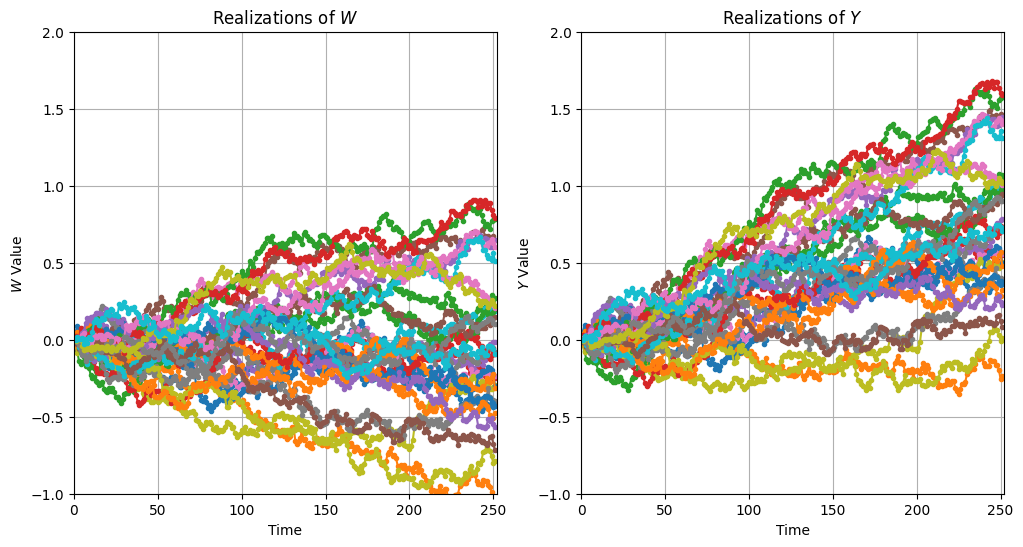
\includegraphics[width=0.45\linewidth]{images/ito_for_girsanov}
		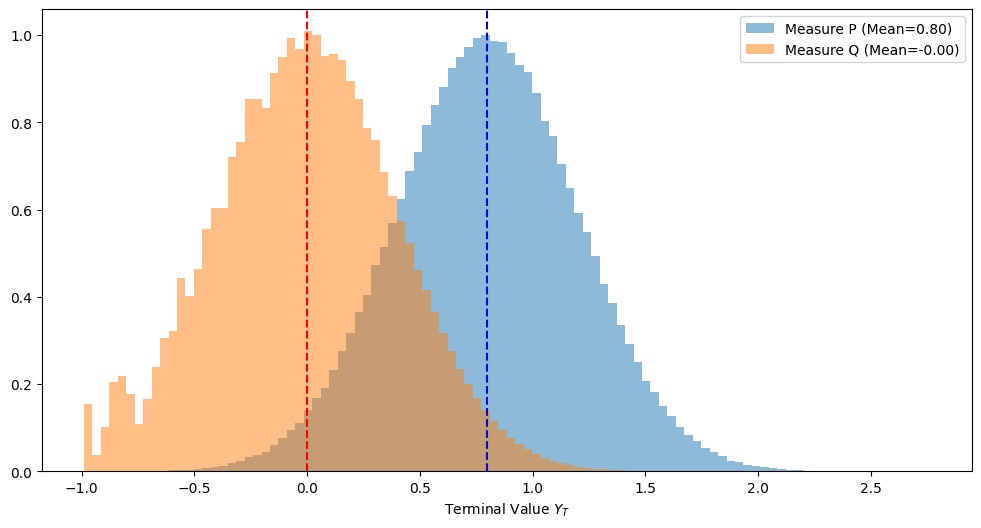
\includegraphics[width=0.25\linewidth]{images/girsanov}
	\end{center}
	
\end{frame}

%\begin{frame}[fragile]{A Trivial Example}
%	First simulate $N=10000$ realizations of a Brownian Motion ($W$) and a of an Ito process ($Y$).
%	\begin{codebox}
	%			\begin{ipython}[linewidth=0.6\linewidth]
		%T = 1
		%M = 252
		%dt = T/M
		%N = 10000
		%mu = 0.8
		%sigma = 0.4
		%
		%epsilon = np.random.normal(size=(M, N))
		%dW = np.sqrt(dt) * epsilon
		%W = np.cumsum(np.vstack([np.zeros(N), dW]), axis=0)
		%dY = mu * dt + sigma * dW
		%Y = np.cumsum(np.vstack([np.zeros(N), dY]), axis=0)
		%			\end{ipython}
	%		\end{codebox}
%	\end{frame}
%
%	\begin{frame}{A Trivial Example}
%		\begin{center}
	%			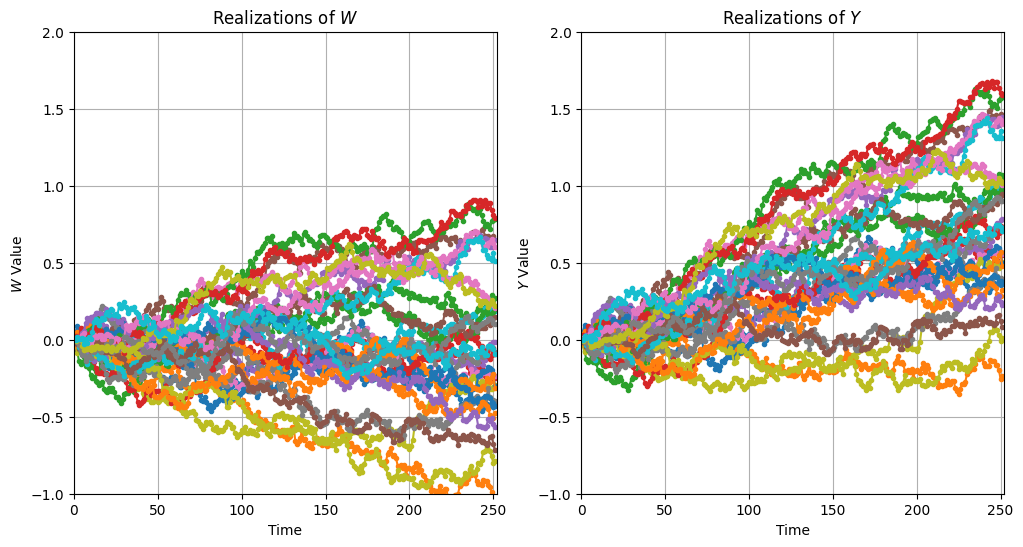
\includegraphics[width=0.9\linewidth]{images/ito_for_girsanov}
	%		\end{center}
%	\end{frame}
%
%	\begin{frame}{A Trivial Example}
%		According to the Girsanov Theorem the Radon-Nikodym derivative in this case becomes $\gamma_t = \cfrac{-\mu}{\sigma}$.
%
%		We have seen that the RN probability distribution tended to assign higher weights to negative values, thus reducing the resulting drift of the process.
%		Using its definition above it is possible to verify the Girsanov theorem, in particular:
%		\begin{enumerate}
	%			\item the original and the transformed process have the same evolution ($\sigma$ is unchanged in the transformation);
	%			\item $\E^{\mathbb{Q}}[Y] = 0$ so the new process is drift-less.
	%		\end{enumerate}
%	\end{frame}
%
%	\begin{frame}[fragile]{A Trivial Example}
%		\begin{columns}
	%			\column{0.5\linewidth}
	%			Define the $RN$ process according to the Girsanov theorem and compute $\E$ and standard deviation for the process $Y$ in the original measure and in the new one (using the Radon-Ninkodym derivative).
	%			\begin{ipython}
		%gamma = -mu/sigma
		%
		%W_T = np.random.normal(0, np.sqrt(T), N)
		%Y_T = mu * T + sigma * W_T
		%
		%zeta_T = np.exp(gamma * W_T - 0.5 * (gamma**2) * T)
		%mean_P = np.mean(Y_T)
		%std_P = np.std(Y_T)
		%mean_Q = np.mean(Y_T * zeta_T)
		%std_Q = np.sqrt(np.mean((Y_T - mean_Q)**2 * zeta_T))
		%\end{ipython}
		%\begin{ioutput}
		%Mean under P: 0.8002 (Expected: 0.8000)
		%Mean under Q: 0.0035 (Expected: 0.0000)
		%Volatility P: 0.4003
		%Volatility Q: 0.3933
		%\end{ioutput}
		%			\column{0.5\linewidth}
		%			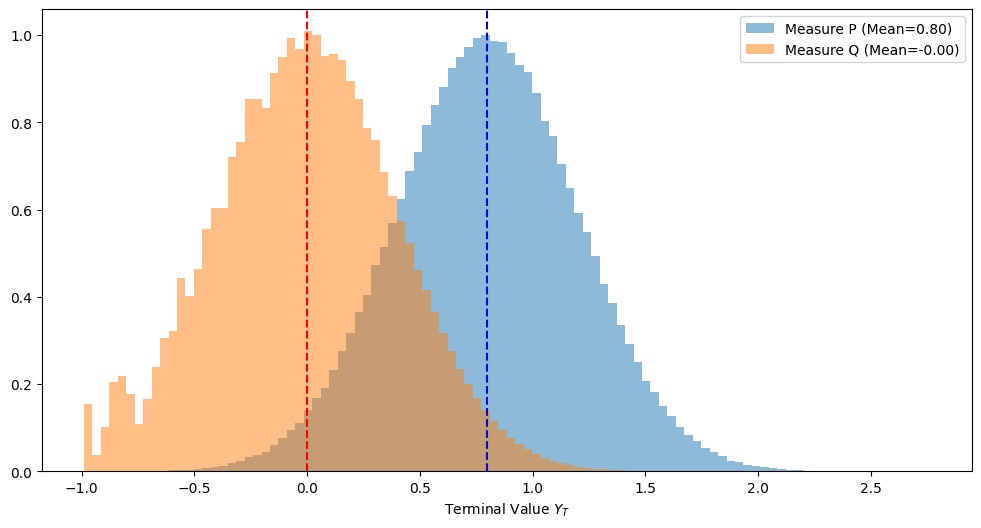
\includegraphics[width=0.9\linewidth]{images/girsanov}
		%		\end{columns}
	%	\end{frame}


%	\begin{homework}
	%		\begin{frame}{\textcolor{white}{Homework}}
		%			\begin{itemize}
			%				\item[white] Consider a stock price which has the following dynamics under the real-world measure $\mathbb{P}$
			%				\begin{equation*}
				%					dS_t = \mu S_t dt + \sigma S_t dW_t
				%				\end{equation*}
			%				Determine what happens to the stock SDE when moving to two different numeraires:
			%				\begin{itemize}
				%					\item[white] risk-neutral measure (bank account numeraire);
				%					\item[white] stock measure (stock numeraire).
				%				\end{itemize}
			%			\end{itemize}
		%		\end{frame}
	%	\end{homework}





%	\begin{frame}[fragile]{Physical vs Risk-Neutral Measure}
	%		\begin{columns}
		%			\column{0.5\linewidth}
		%			Imagine an underlying asset $S$ which currently is valued 100. Simulate $N$ possible realization of the random variable $S$ both under the \textbf{physical} probability measure and the in the \textbf{risk-neutral measure}.
		%
		%			Consider then a 1 year call option on that asset with strike $K=120$. Determine and compare its value using Monte Carlo simulation under both measures.
		%			\column{0.5\linewidth}
		%			\begin{ipython}
			%				import numpy as np
			%
			%				mu = 0.05
			%				r = 0.01
			%				sigma = 0.20
			%				gamma = (mu-r)/sigma
			%				S0 = 100
			%				K = 120
			%				T = 1
			%				M = 365
			%				dt = T/M
			%				N = 100000
			%			\end{ipython}
		%		\end{columns}
	%	\end{frame}
%
%	\begin{frame}[fragile]{Physical vs Risk-Neutral Measure}
	%		\begin{codebox}
		%			\begin{ipython}[linewidth=0.7\linewidth]
			%				dW = np.sqrt(dt)*np.random.normal(size=N*M).reshape(M, N)
			%				SP = np.zeros_like(dW)
			%				SP[0, :] = S0
			%				for t in range(1, M):
			%				SP[t, :] = SP[t-1, :] + mu*dt*SP[t-1, :] + sigma*SP[t-1, :]*dW[t-1, :]
			%
			%				SP_exp = np.mean(SP, axis=1)
			%			\end{ipython}
		%		\end{codebox}
	%		\begin{center}
		%			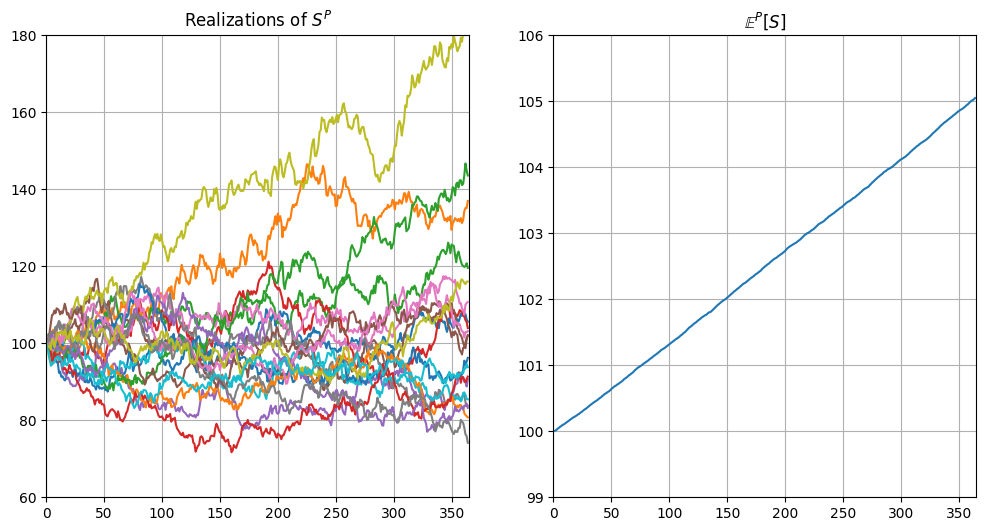
\includegraphics[width=0.60\linewidth]{images/evolution_under_P}
		%		\end{center}
	%	\end{frame}
%
%	\begin{frame}[fragile]{Physical vs Risk-Neutral Measure}
	%		\begin{codebox}
		%			\begin{ipython}[linewidth=0.7\linewidth]
			%				SQ = np.zeros_like(dW)
			%				SQ[0, :] = S0
			%				for t in range(1, M):
			%				SQ[t, :] = SQ[t-1, :] + r*dt*SQ[t-1, :] + sigma*SQ[t-1, :]*dW[t-1, :]
			%
			%				SQ_exp = np.mean(SQ, axis=1)
			%			\end{ipython}
		%		\end{codebox}
	%		\begin{center}
		%			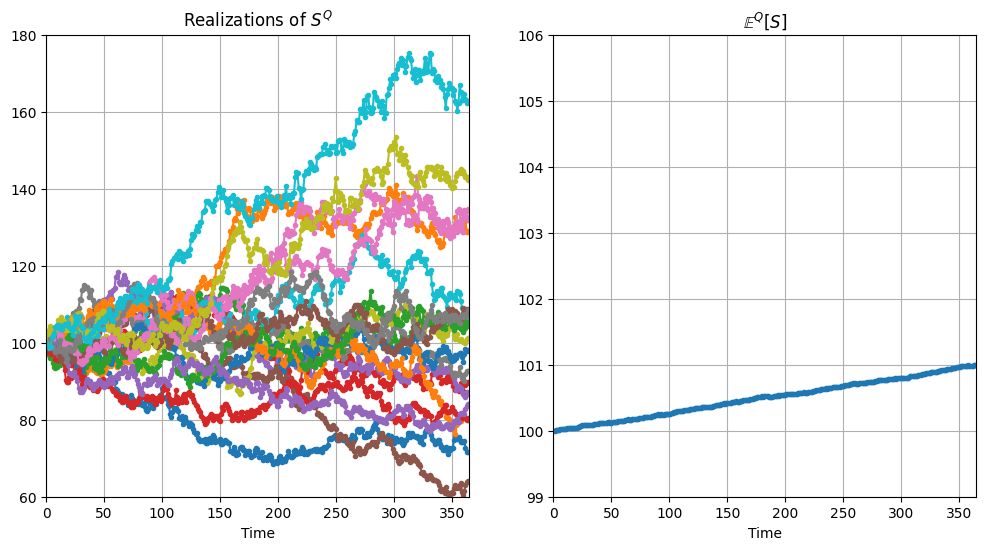
\includegraphics[width=0.60\linewidth]{images/evolution_under_Q}
		%		\end{center}
	%	\end{frame}
%
%	\begin{frame}[fragile]{Physical vs Risk-Neutral Measure}
	%		\begin{columns}
		%			\column{0.7\linewidth}
		%			\begin{ipython}
			%				# sanity check with Radon-Nikodym Derivative
			%
			%				RN = np.ones_like(dW)
			%				for t in range(1, M):
			%				RN[t, :] = np.exp(-gamma*dW[t, :] - 0.5*gamma**2*dt)
			%
			%
			%
			%				# call price calculation under the two measures
			%
			%				CQ = np.exp(-r*T)*np.maximum((SQ[-1, :]-K), 0)
			%				print (f"Price under Q: {np.mean(CQ):.2f}")
			%
			%				CP_RN = np.exp(-r*T)*np.maximum((SP[-1, :]-K), 0)*np.cumprod(RN, axis=0)[-1, :]
			%				print (f"Price under Q (via RN): {np.mean(CP_RN):.2f}")
			%			\end{ipython}
		%			\begin{ioutput}
			%
			%				Price under Q: 2.31
			%				Price under Q (via RN): 2.30
			%			\end{ioutput}
		%			\column{0.3\linewidth}
		%			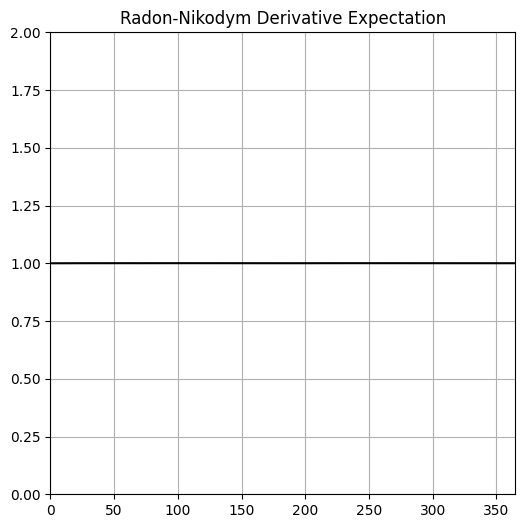
\includegraphics[width=0.80\linewidth]{images/rdn_physical_risk_neutral}
		%			\vspace{1.6cm}
		%		\end{columns}
	%	\end{frame}
%
%	\begin{homework}
	%		\begin{frame}{\textcolor{white}{Homework}}
		%			\begin{itemize}
			%				\item[white] Suppose $W(t)$ is a standard Brownian motion. For each of the following choices of $X_t$, find an equivalent probability measure $\mathbb{Q}$ such that $X_t$ is a Brownian motion in the new measure. Assume $X_0=W_0=0$
			%				\begin{equation*}
				%					\begin{gathered}
					%						dX_t = 2dt + dW_t\\
					%						dX_t = 2dt + 6dW_t
					%					\end{gathered}
				%				\end{equation*}
			%				\item[white] Let $X_t$ be the unique solution to the following stochastic differential equation, under $\mathbb{P}$:
			%				\begin{equation*}
				%					dX_t = X_t(\mu_t dt + \sigma_t dW_t)
				%				\end{equation*}
			%				where $\mu$ and $\sigma$ are bounded and adapted processes, and $\sigma >0$ almost surely.
			%				\begin{itemize}
				%					\item[white] Show that $X_t\exp(-\int_0^t \mu_s ds)$ is a martingale.
				%					\item[white] Find a probability $\mathbb{Q}$, equivalent to $\mathbb{P}$ under which $X$ is a martingale.
				%					\item[white] Find a probability $\tilde{\mathbb{P}}$, equivalent to $\mathbb{P}$, under which the inverse process $X^{-1}$ is a martingale.
				%				\end{itemize}
			%			\end{itemize}
		%		\end{frame}
	%	\end{homework}

\begin{frame}{Drift Changes Generalization}
	\begin{block}{Proposition}
		Assume the following dynamics for a $n$-vector diffusion process $X$ under a generic $N$-measure
		\begin{equation*}
			dX_t = \mu_t^N(X_t)dt + \sigma_t(X_t)CdW^N_t
		\end{equation*}
		where $dW^N_t$ is a $n$-dimensional Brownian motion with correlation matrix $C$. Under the $U$-measure, we have
		\begin{align}
			\mu^U_t(X_t) &= \mu^N_t(X_t) - \rho\sigma(X_t)\left(\frac{\sigma^N_t}{N_t}-\frac{\sigma^U_t}{U_t}\right)' \\
			CdW^U_t &= CdW^N_t + \rho\left(\frac{\sigma^N_t}{N_t}-\frac{\sigma^U_t}{U_t}\right)' dt
		\end{align}
		$\rho=CC'$ is the correlation matrix of $<dW^N_i,dW^N_j>$ and $\sigma^N_t$ and $\sigma^U_t$ are the (vector) volatilities of numeraires $N$ and $U$. %(one component for each Brownian motion).
	\end{block}
\end{frame}

%	\begin{frame}{Drift Changes (Proof)}
	%		%We now provide a formal proof of the above proposition in the special case of \textcolor{maincolor}{$n=1$}, in which \textcolor{maincolor}{$\rho=1$}.
	%
	%		Indicate by $\mathbb{Q}^N$ and $\mathbb{Q}^U$ the $N$-measure and $U$-measure. By Girsanov theorem we have the following expression for the Radon-Nikodym derivative
	%		\begin{equation*}
		%			\zeta_t = \frac{d\mathbb{Q}^N}{d\mathbb{Q}^U} = e^{-\frac{1}{2}\int_0^t\gamma_s^2 ds + \int_0^t\gamma_s dW_s^U}
		%		\end{equation*}
	%		with
	%		\begin{equation}
		%			\gamma_t=\frac{[\mu^N_t(X_t)-\mu_t^U(X_t)]'}{(\sigma_t(X_t)C)'}
		%			\label{eq:gamma_t}
		%		\end{equation}
	%		\pause
	%		We also know that $\zeta_t$ is an exponential martingale hence its dynamics is such that
	%		\begin{equation}
		%			d\zeta_t=\gamma_t\zeta_tdW_t^U
		%			\label{eq:dzeta1}
		%		\end{equation}
	%	\end{frame}
%
%	\begin{frame}{Drift Changes (Proof)}
	%		By the main theorem on numeraire change \cref{eq:radon_nikodym_der2}, and using the fact that $\zeta_t$ is a $\mathbb{Q}^U$-martingale,
	%		\begin{equation}
		%			\zeta_t = \frac{d\mathbb{Q}^N}{d\mathbb{Q}^U} = \frac{U_0N_t}{N_0U_t}
		%			\label{eq:zeta_numeraire}
		%		\end{equation}
	%		thus
	%		\begin{equation}
		%			d\zeta_t= \frac{U_0}{N_0}d\left(\frac{N_t}{U_t}\right)= \frac{U_0}{N_0}\sigma_t^{N/U}CdW_t^U
		%			\label{eq:dzeta2}
		%		\end{equation}
	%		where $\sigma^{N/U}_t$ is the volatility of the process $N_t/U_t$, which is also a martingale under $\mathbb{Q}^U$.
	%	\end{frame}
%
%	\begin{frame}{Drift Changes (Proof)}
	%		Comparing the two results for $d\zeta_t$ (\cref{eq:dzeta1}, \cref{eq:dzeta2} and using \cref{eq:zeta_numeraire}) we get
	%		\begin{equation*}
		%			\begin{gathered}
			%				\gamma_t\zeta_tdW_t^U = \gamma_t\frac{\cancel{U_0}N_t}{\cancel{N_0}U_t}\cancel{dW_t^U}=	\frac{\cancel{U_0}}{\cancel{N_0}}\sigma^{N/U}_tC\cancel{dW_t^U} \implies
			%				\gamma_t = \frac{U_t}{N_t}\sigma^{N/U}_tC
			%			\end{gathered}
		%		\end{equation*}
	%		\pause
	%		Using the definition of $\gamma_t$ (\cref{eq:gamma_t}) and remembering that given two matrices $A$ and $B$ it holds ($(AB)' = B'A'$)
	%		\begin{equation}
		%			\begin{gathered}
			%				(\mu_t^N(X_t)-\mu_t^U(X_t))'= \gamma_t (\sigma_t(X_t)C)'=\frac{U_t}{N_t}\sigma^{N/U}_t CC'(\sigma_t(X_t))'\\
			%				\mu_t^U(X_t)=\mu_t^N(X_t)-\frac{U_t}{N_t}\sigma_t(X_t)\rho(\sigma^{N/U}_t)'
			%			\end{gathered}
		%			\label{eq:gamma}
		%		\end{equation}
	%	\end{frame}
%
%	\begin{frame}{Intermezzo}
	%		\begin{itemize}
		%			\item One of the classical formulas of differential calculus is the Leibniz rule $d(x y) = x(dy) + y(dx)$
		%			\item For stochastic processes this becomes, applying It$\hat{o}$'s formula to the function $F(X,Y) = XY$
		%			\begin{equation*}
			%				dF(x_i)=\sum_{i=1}^n \frac{\partial F}{\partial x_i}dx_i
			%				+\frac{1}{2}\sum_{i,j=1}^2 \frac{\partial^2 F}{\partial x_i \partial x_j}dx_i dx_j
			%			\end{equation*}
		%			For $n=2$:
		%			\begin{equation*}
			%				\begin{gathered}
				%					\frac{\partial F}{\partial X}=Y,\frac{\partial F}{\partial Y}=X \\
				%					\frac{\partial^2 F}{\partial X^2}=0,\frac{\partial^2 F}{\partial X\partial Y}=\frac{\partial^2 F}{\partial Y\partial X}=1,\frac{\partial^2 F}{\partial Y^2}=0\\
				%					\\
				%					d(XY) = XdY + YdX + dXdY
				%				\end{gathered}
			%			\end{equation*}
		%		\end{itemize}
	%	\end{frame}
%
%	\begin{frame}{Drift Changes (Proof)}
	%		Now let $N_t$ and $U_t$ have dynamics under $\mathbb{Q}^U$ given by
	%		\begin{equation*}
		%			\begin{gathered}
			%				dN_t = (\ldots) dt + \sigma_t^NCdW^U_t\\
			%				dU_t = (\ldots) dt + \sigma_t^UCdW^U_t
			%			\end{gathered}
		%		\end{equation*}
	%		\pause
	%		From what we have just seen about the product rule in stochastic calculus
	%		\begin{equation*}
		%			\begin{gathered}
			%				d\left(\frac{N_t}{U_t}\right)=\frac{1}{U_t}dN_t+N_td\frac{1}{U_t}+dN_td\frac{1}{U_t} \quad \left(d\frac{1}{U_t}=-\frac{1}{U^2_t}dU_t+\cancel{\frac{1}{U^3_t}dU_tdU_t}\right) \\
			%			\end{gathered}
		%		\end{equation*}
	%		\pause
	%		Replacing the dynamics for $N_t$ and $U_t$ (ignoring the terms in $dt$ since we know that $d\cfrac{N_t}{U_t}$ is a martingale)
	%		\begin{equation}
		%			d\left(\frac{N_t}{U_t}\right) = \frac{dN}{U_t}-\frac{N_tdU}{U^2_t}\cancel{-\frac{dNdU}{U_t^2}}=\frac{\sigma^N_t CdW^U_t}{U_t} - \frac{N_t\sigma^U_t C dW^U_t}{U^2_t}
		%			\label{eq:dnu}
		%		\end{equation}
	%	\end{frame}
%
%	\begin{frame}{Drift Changes (Proof)}
	%		Taking $d(N_t/U_t)$ definition from \cref{eq:dzeta2} and comparing it with \cref{eq:dnu}
	%		\begin{equation}
		%			d\left(\frac{N_t}{U_t}\right)=\sigma_t^{N/U}\cancel{C dW^U_t} = \frac{\sigma^N_t \cancel{CdW^U_t}}{U_t} - \frac{N_t\sigma^U_t \cancel{C dW^U_t}}{U^2_t}\implies \sigma_t^{N/U}= \frac{\sigma^N_t}{U_t} - \frac{N_t\sigma^U_t}{U^2_t}
		%		\end{equation}
	%		Replacing above expression for $\sigma_t^{N/U}$ into \cref{eq:gamma}
	%		\begin{equation}
		%			\begin{aligned}
			%				\mu_t^U(X_t)&=\mu_t^N(X_t)-\frac{\cancel{U_t}}{N_t}\sigma_t(X_t)\rho\left(\frac{\sigma^N_t}{\cancel{U_t}} - \frac{N_t}{U_t^{\cancel{2}}}\sigma^U_t\right)'\\
			%				&=\mu_t^N(X_t)-\sigma_t(X_t)\rho\left(\frac{\sigma^N_t}{N_t} - \frac{\sigma^U_t}{U_t}\right)'
			%			\end{aligned}
		%		\end{equation}
	%		which proves the \textcolor{maincolor}{first part} of the statement.
	%	\end{frame}
%
%	\begin{frame}{Drift Changes (Proof)}
	%		Expressing $\gamma_t$ coefficient in terms of the numeraires volatilities
	%		\begin{equation*}
		%			\begin{cases}
			%				\gamma_t = \frac{[\mu_t^N(X_t) - \mu_t^U(X_t)]'}{(\sigma_t(X_t)C)'}\\
			%				\mu_t^N(X_t) - \mu_t^U(X_t) = \sigma_t(X_t)\rho \left(\frac{\sigma^N_t}{N_t} - \frac{\sigma^U_t}{U_t}\right)'
			%			\end{cases}\implies \gamma_t = \frac{\left(\frac{\sigma^N_t}{N_t} - \frac{\sigma^U_t}{U_t}\right)CC'(\sigma_t(X_t))}{C'(\sigma_t(X_t))'}
		%		\end{equation*}
	%		\begin{equation}
		%			\gamma_t = \left(\frac{\sigma^N_t}{N_t} - \frac{\sigma^U_t}{U_t}\right)C = C'\left(\frac{\sigma^N_t}{N_t} - \frac{\sigma^U_t}{U_t}\right)'\quad(\text{$C$ is a symmetric matrix})
		%			\label{eq:gamma_3}
		%		\end{equation}
	%		\pause
	%		Finally from the Girsanov theorem we get the diffusion process under the new numeraire
	%		\begin{equation}
		%			\begin{gathered}
			%				CdW^N_t = CdW^U_t - C\gamma_t dt \\
			%				CdW^N_t = CdW^U_t - \rho\left(\frac{\sigma^N_t}{N_t}-\frac{\sigma^U_t}{U_t}\right)' dt
			%			\end{gathered}
		%			\label{eq:girsanov_shock_extended}
		%		\end{equation}
	%		\myendproof
	%
	%		which proves also the \textcolor{maincolor}{second part} of the proposition.
	%
	%		%As an exercise, once you know the Vasicek short rate model, try to determine the new drift when moving from bank account to forward meeasure.%the result is an application of the previous formula with $X = r$, $Q = P^T$ , $\sigma(X_t,t) = \sigma$, $\sigma_B (t) = -A(t, T)\sigma$ and $m(X_t,t) = a(b-rt)$.
	%	\end{frame}













%	\begin{frame}{Asset/Numeraire by Girsanov}
	%		Assuming an asset $S$ and a numeraire $N$ with the following evolutions under the risk-neutral measure
	%		\begin{equation}
		%			\begin{cases}
			%				\cfrac{dS_t}{S_t} = r_tdt + \sigma^S_t dW^B_t\quad\text{(asset)} \\
			%				\cfrac{dN_t}{N_t} = r_tdt + \sigma^N_t dW^B_t\quad\text{(numeraire)}
			%			\end{cases}
		%			\label{eq:S_N_dynamics}
		%		\end{equation}
	%
	%		by Girsanov Theorem (\cref{eq:girsanov_shock_extended}), under $\mathbb{Q}^N$, we get
	%		\begin{equation}
		%			dW^N_t = dW_t^B - \sigma_t^N dt
		%			\label{eq:girsanov_ex}
		%		\end{equation}
	%		which is a Brownian motion.
	%	\end{frame}
%
%	\begin{frame}{Asset/Numeraire by Girsanov}
	%		Now let's apply It$\hat{o}$'s lemma to $S_t/N_t$
	%		\begin{equation*}
		%			\begin{aligned}
			%				d\left(\frac{S}{N}\right) &= \frac{1}{S}dS - \frac{S}{N^2}dN + \frac{S}{N^3}dN^2-\frac{1}{N^2}dSdN = \frac{S}{N}\left(\frac{dS}{S}-\frac{dN}{N}+\frac{dN^2}{N^2}-\frac{dSdN}{SN} \right) = \\
			%				&=\frac{S}{N}\left(rdt+\sigma^S dW^B - rdt - \sigma^N dW^B + (\sigma^N)^2 dt - \sigma^S\sigma^N dt \right) = \quad\textit{(with \cref{eq:S_N_dynamics})}\\
			%				&=\frac{S}{N}((\sigma^N)^2 - \sigma^S\sigma^N) dt + \sigma^S dW^B - \sigma^N dW^B = \quad\textit{(with \cref{eq:girsanov_ex})}\\
			%				&=\frac{S}{N}((\sigma^N)^2 - \sigma^S\sigma^N) dt + \sigma^S (dW^N + \sigma^N dt) - \sigma^N(dW^N+\sigma^Ndt) = \\
			%				&=\frac{S}{N}(\sigma^S - \sigma^N)dW^N
			%			\end{aligned}
		%		\end{equation*}
	%		which shows that $\cfrac{S}{N}$ is a $\mathbb{Q}^N$-martingale (no drift in dynamics).
	%	\end{frame}

\begin{frame}{The Vasicek Model under $\mathbb{P}$ \colablink{https://colab.research.google.com/drive/1RruIgCzM4AwQ8TH7uPIJIOf-y-oFLDHg}}
	\begin{itemize}
		\item Statistical analysis of historical interest rate data suggests that rates are mean-reverting. Under the physical measure $\mathbb{P}$, we model the short rate $r_t$ as:
		\begin{equation*}
			dr_t = a(b-rt)dt + \sigma W_t^\mathbb{P}
		\end{equation*}
		where $a$ speed of mean reversion, $b$ long-term mean level, $\sigma$ volatility, and $W_t^\mathbb{P}$ Brownian motion \textbf{under the real-world measure}.
		\item If we use these parameters to price a bond via $\E^\mathbb{P}[\exp(-\int r_s ds)]$, we are assuming investors are risk-neutral towards interest rate volatility.
		\item But the bond is a risky asset and investors will not buy it unless the price is lower than the mathematical average of discounted cash-flows, i.e. $\E^\mathbb{P}$ is for forecasting, not pricing.
		\item \textbf{Investors demand a premium for bearing interest rate risk}.
	\end{itemize}
\end{frame}

\begin{frame}{Market Price of Risk}
	\begin{itemize}
		\item The \emph{Market Price of Risk} $\lambda$ represents the extra return (drift) investors demand per unit of risk they take on.
		\item Girsanov’s Theorem allows us to mathematically "subtract" this compensation from the real-world drift, leaving us with a process that can be priced as if the world were risk-neutral
		\begin{equation*}
			dW_t^\mathbb{Q} = dW_t^\mathbb{P} + \lambda dt \implies dW_t^\mathbb{P} = dW_t^\mathbb{Q} - \lambda dt
		\end{equation*}
		\item Substituting this into the $\mathbb{P}$-dynamics:
		\begin{equation*}
			dr_t = a(b-rt)dt + \sigma(dW_t^\mathbb{Q}-\lambda dt)
		\end{equation*}
		
	\end{itemize}
\end{frame}

\begin{frame}{The Risk-Neutral Dynamics}
	\begin{itemize}
		\item Grouping the $dt$ terms from the previous slide:
		\begin{equation*}
			dr_t=[a(b-rt)-\sigma\lambda]dt+\sigma dW_t^\mathbb{Q}
		\end{equation*}
		\item To maintain the mean-reverting structure $dr_t=a^*(b^*-rt)dt+\sigma dW_t^\mathbb{Q}$, we distribute the terms:
		\begin{equation*}
			dr_t=[ab-ar_t-\sigma\lambda]dt+\sigma dW_t^\mathbb{Q} =\overbrace{a}^{a^*} \bigg[\overbrace{\left(b-\frac{\sigma\lambda}{a}\right)}^{b^*}-rt\bigg]dt+\sigma dW_t^\mathbb{Q}
		\end{equation*}
		where the speed of reversion remains unchanged, and the long-term mean $b^* = b - \frac{\sigma \lambda}{a}$ is shifted.
		\item If $\lambda < 0$ then $b^* > b$.
		The market "prices" bonds as if the long-term interest rate is higher than what we see in historical data.
		This compensates the bond buyer for the interest rate risk.
	\end{itemize}
\end{frame}

\begin{frame}{Numerical Results }
	\begin{columns}
		\column{0.4\linewidth}
		\begin{itemize}
			\item \textcolor{blue}{The Blue Line ($\mathbb{P}$)}: "Best Guess" based on history.
			\item \textcolor{red}{The Red Line ($\mathbb{Q}$)}: "Pricing Guess" investors are afraid of interest rate, they price bonds as if rates are lower.
			\item The vertical distance between the blue and red lines is where the Market Price of Risk lives.
		\end{itemize}
		\column{0.6\linewidth}
		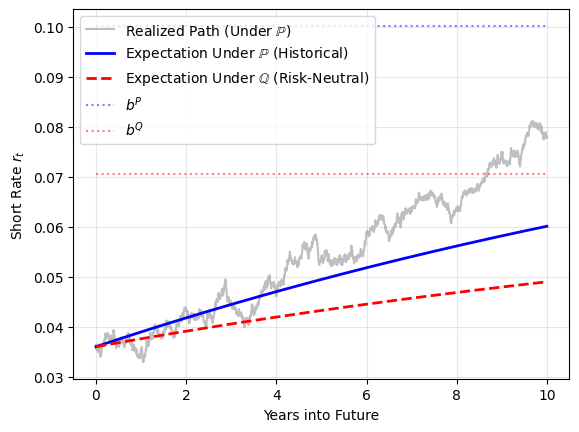
\includegraphics[width=0.9\linewidth]{images/vasicek_under_P}
	\end{columns}
	\vfill
	We aren't changing the math of mean reversion; we are just changing the destination ($b\to b^*$) to ensure our model matches the market prices.
\end{frame}

\begin{frame}{Why Girsanov is Essential Here}
	\begin{itemize}
		\item Without Girsanov we would simply know that \emph{prices are expectations}, but we wouldn't know which interest rate process to simulate.
		\item With Girsanov we have a specific recipe. We take our historical $b$, subtract the risk adjustment $\frac{\sigma\lambda}{a}$, and we have a ready-to-use SDE for Monte Carlo or the Riccati equations.
		\item The Radon-Nikodym derivative that makes this happen is:
		\begin{equation*}
			\frac{d\mathbb{P}}{d\mathbb{Q}}=\exp\left(-\frac{1}{2}\int_0^T\lambda^2 dt - \int_0^T\lambda dW_t^\mathbb{P}\right)
		\end{equation*}
	\end{itemize}
\end{frame}

\section{Convexity}
\begin{frame}{Convexity Correction}
	\begin{itemize}
		\item<1-> In financial lingo, convexity is a broadly understood and often non-specific term for nonlinear behavior of the price of an instrument as a function of evolving markets.
		\item<2-> The concept of \emph{convexity adjustment} is required for all asset classes when there are payment delays or when the payment dates of the contract do
		not correspond to those used in the numeraire defintion.
		\item<3-> From the perspective of financial modeling they arise as the results of valuation done under the \emph{"wrong"} measure.
		\item<4-> The higher the uncertainty in the market (high volatility) the more pronounced the effect of the convexity will become.
	\end{itemize}
\end{frame}

\begin{frame}{The Good\ldots}
	\begin{itemize}
		\item<1-> Let us consider a basic interest rate payoff function, whose payoff depends on the EURIBOR rate
		\begin{equation*}
			V(t_0) = N\cdot D(t_0)\cdot\expect{Q}\left[\cfrac{F(T_{i-1};T_{i-1},T_i)}{D(T_i)}\right]=
			N\cdot P(t_0,T_i)\cdot\mathbb{E}^{T_i}[F(T_{i-1};T_{i-1},T_i)]
		\end{equation*}
		\item<2-> Since $F_{i}(T_{i-1}) = F(T_{i-1};T_{i-1}, T_i)$ is a martingale under the $T_i$-forward measure, we get
		\begin{equation*}
			V(t_0)= N\cdot P(t_0,T_i)\cdot F_i(t_0)
		\end{equation*}
	\end{itemize}
\end{frame}

\begin{frame}{\ldots and the Bad}
	\begin{itemize}
		\item<1-> Imagine now a similar contract where, however, the payments will take place at some earlier time $T_{i-1} < T_i$. \item<2->Its current value is given by
		\begin{equation*}
			V(t_0) = N\cdot D(t_0)\cdot\expect{Q}\left[\cfrac{F_i(T_{i-1})}{D(T_{i-1})}\right]
		\end{equation*}
		\item<3-> When changing measure (to the $T_{i-1}$-forward measure) we get the following Radon-Nikodym derivative:
		\begin{equation*}
			\cfrac{d\mathbb{Q}^{T_{i-1}}}{d\mathbb{Q}}=\cfrac{P(T_{i-1},T_{i-1})D(t_0)}{P(t_0,T_{i-1})D(T_{i-1})}
		\end{equation*}
		\item<4->So that
		\begin{equation*}
			V(t_0) = N\cdot D(t_0)\cdot\expect{Q}\left[\cfrac{F_i(T_{i-1})}{D(T_{i-1})}\right] = N\cdot D(t_0)\cdot\mathbb{E}^{T_{i-1}}\left[\cfrac{P(t_0,T_{i-1})D(T_{i-1})}{P(T_{i-1},T_{i-1})D(t_0)}\cfrac{F_i(T_{i-1})}{D(T_{i-1})}\right]
		\end{equation*}
	\end{itemize}
\end{frame}

\begin{frame}{The Correction}
	\begin{itemize}
		\item<1-> After few simplifications
		\begin{equation*}
			\begin{aligned}
				V(t_0) = N\cdot \cancel{D(t_0)}\cdot\mathbb{E}^{T_{i-1}}&\left[\cfrac{P(t_0,T_{i-1})\cancel{D(T_{i-1})}}{P(T_{i-1},T_{i-1})\cancel{D(t_0)}}\cfrac{F_i(T_{i-1})}{\cancel{D(T_{i-1})}}\right] = \\
				&= N\cdot P(t_0,T_{i-1})\cdot\mathbb{E}^{T_{i-1}}[F_i(T_{i-1})]
			\end{aligned}
		\end{equation*}
		\item<1-> Although the Libor rate is a martingale under the $T_i$-forward
		measure, it is however \textbf{not} a martingale under the $T_{i-1}$-forward measure, i.e.,
		\begin{equation*}
			\mathbb{E}^{T_{i-1}}\left[F_i(T_{i-1})\right]\neq \mathbb{E}^{T_i}\left[F_i(T_{i-1})\right] = F_i(t_0)
		\end{equation*}
		\item<2-> The difference between these two expectations is commonly referred to as a \textbf{convexity}.
	\end{itemize}
\end{frame}

\begin{frame}{Changing Measures}
	\begin{itemize}
		\item<1-> By the change of measure technique, we can simplify the expressions above, to some extent.
		\item<2-> Indeed moving to the $T_i$-forward measure, we find:
		\begin{equation*}
			\cfrac{d\mathbb{Q}^{T_{i-1}}}{d\mathbb{Q}^{T_i}}=\cfrac{P(t_0,T_i)P(T_{i-1},T_{i-1})}{P(T_{i-1},T_i)P(t_0,T_{i-1})}
		\end{equation*}
		\item<3-> The derivative value is then equal to
		\only<3-3>{\begin{equation*}
				\begin{aligned}
					V(t_0) &= N\cdot P(t_0,T_{i-1})\cdot\mathbb{E}^{T_{i-1}}[F_i(T_{i-1})] = \\
					&=N\cdot P(t_0,T_{i-1})\cdot\mathbb{E}^{T_i}\left[F_i(T_{i-1})\cfrac{P(t_0,T_i)P(T_{i-1},T_{i-1})}{P(T_{i-1},T_i)P(t_0,T_{i-1})}\right]=\\
				\end{aligned}
		\end{equation*}}
		\only<4-4>{\begin{equation*}
				\begin{aligned}
					V(t_0) &= N\cdot P(t_0,T_{i-1})\cdot\mathbb{E}^{T_{i-1}}[F_i(T_{i-1})] = \\
					&=N\cdot \cancel{P(t_0,T_{i-1})}\cdot\mathbb{E}^{T_i}\Bigg[F_i(T_{i-1})\cfrac{P(t_0,T_i)\overbrace{P(T_{i-1},T_{i-1})}^{=1}}{P(T_{i-1},T_i)\cancel{P(t_0,T_{i-1})}}\Bigg]=\\
				\end{aligned}
		\end{equation*}}
		\only<5->{\begin{equation*}
				\begin{aligned}
					V(t_0) &= N\cdot P(t_0,T_{i-1})\cdot\mathbb{E}^{T_{i-1}}[F_i(T_{i-1})] = \\
					&=N\cdot \mathbb{E}^{T_i}\left[F_i(T_{i-1})\cfrac{P(t_0,T_i)}{P(T_{i-1}, T_i)}\right]\\
				\end{aligned}
		\end{equation*}}
	\end{itemize}
\end{frame}

\begin{frame}{The Correction}
	\begin{itemize}
		\item<1-> By adding and subtracting $F_i(T_{i-1})$ and splitting the expectation can be rewritten as
		\begin{equation*}
			\begin{aligned}
				V(t_0) &= N\cdot \mathbb{E}^{T_i}\left[F_i(T_{i-1}) + F_i(T_{i-1})\cfrac{P(t_0,T_i)}{P(T_{i-1}, T_i)} - F_i(T_{i-1})\right] \\
				&= N\cdot \mathbb{E}^{T_i}[F_i(T_{i-1})] + N\cdot \mathbb{E}^{T_i}\left[F_i(T_{i-1})\left(\cfrac{P(t_0,T_i)}{P(T_{i-1}, T_i)}-1\right)\right]\\
				&=N\cdot\Bigg(F_i(t_0) + \underbrace{\mathbb{E}^{T_i}\left[F_i(T_{i-1})\left(\cfrac{P(t_0,T_i)}{P(T_{i-1}, T_i)}-1\right)\right]}_{\text{convexity correction}}\Bigg)
			\end{aligned}
		\end{equation*}
		\item<2-> The convexity correction can finally be expressed as
		\begin{equation}
			\boxed{
				P(t_0,T_i)\mathbb{E}^{T_i}\left[\cfrac{F_i(T_{i-1})}{P(T_{i-1},T_i)}\right]-F_i(t_0)}
		\end{equation}
	\end{itemize}
\end{frame}

\begin{frame}{Final Remark}
	\begin{itemize}
		\item<1-> From the definition of EURIBOR rate: $P(T_{i-1},T_i)=\cfrac{1}{1+\tau_i F_i(T_{i-1})}$ hence
		\begin{equation*}
			\mathbb{E}^{T_i}\left[\cfrac{F_i(T_{i-1})}{P(T_{i-1},T_i)}\right]=F_i(t_0)+\tau_i\mathbb{E}^{T_i}[F_i^2(T_{i-1})]
		\end{equation*}
	\end{itemize}
	\vfill
	\begin{tcolorbox}[colback=gray!5, colframe=maincolor, arc=0mm, boxrule=0.5pt]
		\footnotesize
		Note that although $F_i(T_{i-1})$ is a martingale under the $T_i$-forward measure, \textbf{its square is not}.
		Indeed applying \ito~lemma to $F_i^2$ with the  dynamics $dF_i(t) = \sigma F_i(t)dW(t)$, give us
		\begin{equation*}
			dF_i^2=\sigma^2F_i^2dt+2\sigma F_i^2dW
		\end{equation*}
		which has a drift term, so it is not a martingale.
	\end{tcolorbox}
	
\end{frame}

\subsection{In Arrears Swap}
\begin{frame}{In-Arrears Swap}
	\begin{itemize}
		\item<1-> An \emph{in-arrears swap} is an IRS that resets and pays at the same dates $\{T_{\alpha+1},\ldots, T_\beta\}$ and with fixed-leg rate $K$. More precisely, the value of a payer IAS is
		\begin{equation}
			\textbf{IAS}=\expect{Q}\left[\sum_{i=\alpha+1}^{\beta}D(0,T_i)\tau_{i+1}(F_{i+1}(T_i)-K)\right]
		\end{equation}
		\item<2-> To compute the expectation we can proceed as follows
		\begin{equation*}
			\begin{aligned}
				\expect{Q}\Bigg[\sum_{i=\alpha+1}^{\beta}D(0,T_i)\tau_{i+1}&(F_{i+1}(T_i)-K)\Bigg] = \\
				&=\expect{Q}\left[\sum_{i=\alpha+1}^{\beta}D(0,T_i)\left(\cfrac{1}{P(T_i,T_{i+1})}-(1+\tau_{i+1}K)\right)\right]=\ldots
			\end{aligned}
		\end{equation*}
	\end{itemize}
\end{frame}

\begin{frame}{In-Arrears Swap}
	\begin{itemize}
		\item<1-> To further simplify the previous expression it is convenient to use the following result from the \emph{tower property} of the expectation:
		\begin{equation*}
			\begin{aligned}
				&\mathbb{E}_t\left[\cfrac{XD(t,S)}{P(T,S)} \right]=\mathbb{E}_t\left[\mathbb{E}_T\left[\cfrac{XD(t,T)D(T,S)}{P(T,S)} \right]\right]=\mathbb{E}_t\left[\cfrac{XD(t,T)}{P(T,S)}\mathbb{E}_T[D(T,S)]\right]= \\
				& =\mathbb{E}_t\left[\cfrac{XD(t,T)}{P(T,S)}P(T,S)\right]=\mathbb{E}_t[XD(t,T)],\quad (t<T<S)
			\end{aligned}
		\end{equation*}
		\item<2-> Then it becomes (with $t=0$, $T=T_i$, $S=T_{i+1}$ and $X=1/P(T_i,T_{i+1})$):
		\begin{equation*}
			\begin{aligned}
				\ldots=\expect{Q}\Bigg[\sum_{i=\alpha+1}^{\beta}&\left(\cfrac{D(0,T_i)}{P(T_i,T_{i+1})}-D(0,T_i)(1+\tau_{i+1}K)\right)\Bigg] = \\
				&=\expect{Q}\left[\sum_{i=\alpha+1}^{\beta}\left(\cfrac{D(0,T_{i+1})}{P(T_i,T_{i+1})^2}-D(0,T_i)(1+\tau_{i+1}K)\right)\right] = \ldots
			\end{aligned}
		\end{equation*}
	\end{itemize}
\end{frame}

\begin{frame}{In-Arrears Swap}
	\begin{itemize}
		\item<1-> From the linearity of the expectation operator and the definition of ZCB price:
		\begin{equation*}
			\begin{aligned}
				\ldots &=\sum_{i=\alpha+1}^{\beta}\left(\expect{Q}\left[\cfrac{D(0,T_{i+1})}{P(T_i,T_{i+1})^2}\right]-\expect{Q}\left[D(0,T_i)(1+\tau_{i+1}K)\right]\right) = \\
				&=\sum_{i=\alpha+1}^{\beta}\left(\expect{Q}\left[\cfrac{D(0,T_{i+1})}{P(T_i,T_{i+1})^2}\right]-P(0,T_i)(1+\tau_{i+1}K)\right) = \ldots\\
			\end{aligned}
		\end{equation*}
		\item<2-> Before computing the remaining expectation let's make a change of measure from the risk-neutral to $P(\cdot, T_{i+1})$
		\only<2-2>{
			\begin{equation*}
				\ldots=\sum_{i=\alpha+1}^{\beta}\Bigg(\mathbb{E}^{T_{i+1}}\Bigg[\cfrac{D(0,T_{i+1})}{P(T_i,T_{i+1})^2}\underbrace{\cfrac{D(T_{i+1},T_{i+1})P(0,T_{i+1})}{D(0,T_{i+1})P(T_{i+1},T_{i+1})}}_{\text{Radon-Nikodym derivative}}\Bigg]-P(0,T_i)(1+\tau_{i+1}K)\Bigg)
				%&=\sum_{i=\alpha+1}^{\beta}\left[P(0,T_{i+1})\mathbb{E}^{i+1}\left[\cfrac{1}{P(T_i,T_{i+1})^2}\right]-P(0,T_i)(1+\tau_{i+1}K)\right] = \\
				%&=\sum_{i=\alpha+1}^{\beta}\left[P(0,T_{i+1})\mathbb{E}^{i+1}\left[(1+\tau_{i+1}F_{i+1}(T_i))^2\right]-P(0,T_i)(1+\tau_{i+1}K)\right]
				%\end{aligned}
		\end{equation*}}
		\only<3->{
			\begin{equation*}
				\ldots=\sum_{i=\alpha+1}^{\beta}\Bigg(\mathbb{E}^{T_{i+1}}\Bigg[\cfrac{\cancel{D(0,T_{i+1})}}{P(T_i,T_{i+1})^2}\cfrac{\overbrace{D(T_{i+1},T_{i+1})}^{=1}P(0,T_{i+1})}{\cancel{D(0,T_{i+1})}\underbrace{P(T_{i+1},T_{i+1})}_{=1}}\Bigg]-P(0,T_i)(1+\tau_{i+1}K)\Bigg)
		\end{equation*}}
	\end{itemize}
\end{frame}

\begin{frame}{In-Arrears Swap}
	\begin{itemize}
		\item<1-> Finally
		\begin{equation}
			\begin{split}
				\textbf{IAS}&=\sum_{i=\alpha+1}^{\beta}\Bigg(P(0,T_{i+1})\mathbb{E}^{T_{i+1}}\Bigg[\cfrac{1}{P(T_i,T_{i+1})^2}\Bigg]-P(0,T_i)(1+\tau_{i+1}K)\Bigg) \\
				&=\sum_{i=\alpha+1}^{\beta}\Bigg(P(0,T_{i+1})\mathbb{E}^{T_{i+1}}[(1+\tau_{i+1}F_{i+1}(T_i))^2]-P(0,T_i)(1+\tau_{i+1}K)\Bigg)
				\label{eq:exp_ias}
			\end{split}
		\end{equation}
		\item<2-> Now it is relatively easy to compute the expectation in Eq.~\ref{eq:exp_ias}, since under $\mathbb{Q}^{T_{i+1}}$, $F_{i+1}$ is a martingale.
		\uncover<3->{so that (using \ito's isometry),
			\begin{equation*}
				\mathbb{E}^{T_{i+1}}[F_{i+1}^2(T_i)]=F_{i+1}^2(0)\exp\left(\int_0^{T_i}\sigma_{i+1}^2(t)dt\right) = F_{i+1}^2(0)\exp(v_{i+1}^2)
			\end{equation*}
			where the $v$ can be determined from cap market prices.}
	\end{itemize}
\end{frame}

\begin{frame}{In-Arrears Swap}
	\begin{itemize}
		\item<1-> The final expression is
		\begin{equation}
			\begin{gathered}
				\textbf{IAS} = \sum_{i=\alpha+1}^{\beta}(P(0,T_{i+1})\mathbb{E}^{T_{i+1}}[(1+\tau_{i+1}F_{i+1}(T_i))^2]-P(0,T_i)(1+\tau_{i+1}K)) \\
				=\sum_{i=\alpha+1}^{\beta}[
				P(0,T_{i+1}) [1+2\tau_{i+1}F_{i+1}(0) + \tau_{i+1}^2 F_{i+1}^2(0)\exp(v_{i+1}^2)]\\
				-(1+\tau_{i+1}K)P(0,T_i)] \\
			\end{gathered}
			\label{eq:ias_price}
		\end{equation}
		\item<2-> From~\cref{eq:ias_price} it is apparent how the valuation results in a vanilla swap-like part plus the convexity correction due to the arrears feature.
		\item<3-> Also, contrary to the plain-vanilla case, the In-Arrear Swap value depends on the volatility of forward rates through the volatilities $v$.
		\item<4-> Notice however that correlations between different rates are not involved in this product, as expected by the nature of the contract.
	\end{itemize}
\end{frame}


\begin{frame}{What is a Quanto?}
	\begin{itemize}
		\item A \emph{quanto} is a "Quantity Adjusting" option/derivative.
		\item An investor wants exposure to a foreign asset (e.g., Nikkei 225) but wants the payoff settled in her domestic currency (e.g., EUR) at a fixed exchange rate,
		to eliminate exchange rate risk while maintaining asset exposure.
		\item The pricing challenge is that we cannot simply use the foreign risk-neutral expectation because the domestic investor lives in a different "measure".
		\item We define two economies:
		\begin{itemize}
			\item Foreign ($F$): risk-free rate $r_f$. Asset price $S_t$ (in foreign currency).
			\item Domestic ($D$): risk-free rate $r_d$.
			\item Exchange Rate ($X_t$): units of domestic currency per 1 unit of foreign currency (e.g., EUR/USD).
			\item The Fixed Rate ($\tilde{X}$): the pre-agreed exchange rate for the payoff.
		\end{itemize}
		\item The Payoff at $T$:
		\begin{equation}
			V_T=\tilde{X}\cdot S_T
		\end{equation}
	\end{itemize}
\end{frame}

\begin{frame}{The SDEs under Foreign Measure $\mathbb{Q}^F$}
	\begin{itemize}
		\item Under the foreign risk-neutral measure $\mathbb{Q}^F$, the asset $S_t$ grows at the foreign risk-free rate:
		\begin{equation}
			dS_t= r_f S_t dt + \sigma_S S_t dW_t^S
		\end{equation}
		\item To find $V_t$ under the domestic measure $\mathbb{Q}^D$ we must look at how the exchange rate $X_t$ behave:
		\begin{equation}
			dX_t=(r_d-r_f)X_t dt + \sigma_X X_t dW_t^X
			\label{eq:exchange_rate_process}
		\end{equation}
		\textbf{Note} that although the exchange rate is fixed we still need its evolution for the change of measure.
		\item We also need to take into account the correlation: $dW_t^S\cdot dW_t^X = \rho dt$ between the foreign asset and the exchange rate:
		\begin{itemize}
			\item $\rho >0$: when the foreign stock goes up, the foreign currency tends to strengthen against the domestic currency (e.g., S\&P 500 goes up and USD gets stronger vs EUR).
			\item $\rho <0$: when the foreign stock goes up, the foreign currency tends to weaken (often seen in "safe-haven" currencies like the Japanese Yen).
		\end{itemize}
	\end{itemize}
\end{frame}

\begin{frame}{Why $(r_d-r_f)$ ?}
	\begin{itemize}
		\item The explain \cref{eq:exchange_rate_process} (defined under $\mathbb{Q}^D$) consider a domestic investor who buys 1 unit of foreign currency. To hold this "asset," the investor effectively invests it in the foreign money market to earn $r_f$.
		\item The total domestic value of this investment at time $t$ is $V_t = X_t e^{r_f t}$.
		\item For the No-Arbitrage Principle, $V_t$ must be a martingale when discounted by $r_d$. Therefore, the discounted process $e^{-r_d t}X_t e^{r_f t}=X_t e^{(r_f-r_d)t}$ must have zero drift.
		\item If we assume $X_t$ follows a GBM then by It$\hat{o}$'s Lemma  to $f(X,t) = X e^{(r_f - r_d)t}$
		\begin{itemize}
			\item $\frac{\partial f}{\partial t} = (r_f - r_d)\tilde{V}_t$; \quad $\frac{\partial f}{\partial X} dX_t = e^{(r_f - r_d)t}(\mu_X X_t dt + \sigma_X X_t dW_t)$
		\end{itemize}
		\item 	The drift of $d\tilde{V}_t$ must vanish:
		\[ (r_f - r_d) + \mu_X = 0 \implies \mu_X = r_d - r_f \]
	\end{itemize}
\end{frame}

\begin{frame}{The Change of Measure Logic}
	\begin{itemize}
		\item The Radon-Nikodym derivative to move from $\mathbb{Q}^F$ to $\mathbb{Q}^D$ is %linked to the volatility of the exchange rate.
		\begin{equation}
			\zeta_t = \frac{d\mathbb{Q}^D}{d\mathbb{Q}^F} = \frac{X_t e^{r_f t}}{X_0 e^{r_d t}} = \frac{X_t}{X_0} e^{(r_f - r_d)t}
		\end{equation}
		\item Under $\mathbb{Q}^D$, the asset $S_t$ does not grow at $r_f$. It acquires a "covariance term" because the domestic investor views the foreign asset through the "lens" of the exchange rate.
		\item Applying the Girsanov Theorem, the new SDE under $\mathbb{Q}^D$ is:
		\begin{equation}
			dS_t=(r_f-\rho\sigma_S\sigma_X)S_t dt + \sigma_S S_t dW_t^D
		\end{equation}
	\end{itemize}
\end{frame}

\begin{frame}{The "Quanto Adjustment": $-\rho\sigma_S\sigma_X$}
	\begin{itemize}
		\item Imagine a Euro-based investor buying a US stock ($S$) paid in EUR at a fixed rate:
		\begin{itemize}
			\item if the stock and the USD/EUR exchange rate are positively correlated ($\rho>0$), the stock tends to go up when the USD is strong.
			\item in a standard (non-quanto) investment, the investor would benefit twice (higher stock price AND stronger currency).
			\item in a Quanto, the investor has "given up" the currency gain (because the rate is fixed at $\tilde{X}$).
		\end{itemize}
		\item If the foreign currency strengthens when the stock rises ($\rho > 0$), the domestic investor "loses" the currency gain due to the fixed exchange rate, so the expected return must be adjusted downwards.
	\end{itemize}
	The value of a Quanto Forward at time $t$ is:
	\begin{equation}
		\boxed{V_t=\tilde{X}S_t e^{(r_f-\rho\sigma_S\sigma_X-r_d)(T-t)}}
	\end{equation}
\end{frame}

\begin{frame}{Extracting Implied Correlation}
	Since $\sigma_S$ and $\sigma_X$ are observable from options, but $\rho$ is not, how can we use Quanto prices to "extract" the market's view on the correlation between e.g. Nikkei 225 and USD/JPY?
	
	\begin{itemize}
		\item \textbf{Step 1:} observe $\sigma_S$ from Nikkei vanilla options (in JPY).
		\item \textbf{Step 2:} observe $\sigma_X$ from USD/JPY FX options.
		\item \textbf{Step 3:} observe the market price of the \textbf{Quanto Nikkei Option} (in USD).
	\end{itemize}
	
	Using the Quanto pricing formula:
	\[ P_{Mkt}^{Quanto} = \text{BS}(\sigma_S, \sigma_X, r_f, \mathbf{\rho_{implied}}) \]
	We solve for $\rho_{implied}$ to see the market's expectation of the Nikkei-Yen relationship.
	
	This allows traders to spot "Correlation Skew" and price path-dependent structures that are sensitive to joint Equity-FX moves.
\end{frame}

\subsection{Siegel's Paradox and Measure Consistency}

\begin{frame}{Siegel's Paradox}
	\emph{If the EUR/USD exchange rate ($X_t$) is a martingale under a certain measure, can the USD/EUR rate ($1/X_t$) also be a martingale ?}
	
	\begin{itemize}
		\item<2-> Assume that under the domestic measure $\mathbb{Q}^D$, the exchange rate $X_t$ follows a Geometric Brownian Motion (with zero drift for simplicity):
		\[ dX_t = \sigma_X X_t dW_t \]
		\item<2-> Applying Itô's Lemma to $Y_t = 1/X_t$ ($Y' = -1/X^2, Y'' = 2/X^3$):
		\begin{equation*}
			dY_t = -\frac{1}{X_t^2}(dX_t) + \frac{1}{2}\frac{2}{X_t^3}(dX_t)^2 \implies
			dY_t = \sigma_X^2 Y_t dt - \sigma_X Y_t dW_t
		\end{equation*}
		
		\item<2-> Even if $X$ has no drift, its inverse $1/X$ has a \textbf{positive drift} equal to its variance $\sigma_X^2$.
		\item<3-> \textbf{The Paradox:} how can one side see a fair game while the other sees a winning game ?
	\end{itemize}
\end{frame}

\begin{frame}{Girsanov and Market Consistency}
	Why is there no arbitrage? It might seem everyone profits by swapping currencies, but Girsanov's Theorem ensures market coherence through a mandatory change of measure.
	
	\begin{itemize}
		\item Under $\mathbb{Q}^D$ (Domestic Investor), the foreign asset $X$ has drift $r_d - r_f$.
		\item When switching to the Foreign Investor's perspective ($\mathbb{Q}^F$), we do not just flip the asset; we \textbf{change the probability measure}.
		\item The transition from $\mathbb{Q}^D$ to $\mathbb{Q}^F$ introduces a drift term that exactly cancels the convexity surplus ($\sigma_X^2$).
		\item International markets remain consistent because "expected returns" are only defined relative to a specific numeraire and its associated measure.
	\end{itemize}
\end{frame}

\begin{frame}{Conclusion: Resolving the Paradox \colablink{https://colab.research.google.com/drive/1DAFTB_xnuIHJ3_ApPKltvJLRfzvOUomH}}
	\begin{itemize}
		\item Itô's Lemma and Jensen's Inequality create a \textit{mathematical drift} in the inverse exchange rate.
		\item This suggests a "free lunch" where both parties expect to gain by holding foreign currency.
		\item Girsanov's Theorem ensures that this drift is exactly offset by the change in the risk-neutral measure.
	\end{itemize}
	\vfill
	\begin{tcolorbox}[colback=gray!5, colframe=maincolor, arc=0mm, boxrule=0.5pt]
		\footnotesize
		Expectations are \textbf{measure-dependent}. What looks like a drift in one measure is merely the cost of the numeraire change in the other. No arbitrage exists.
		
		\[ \text{Price}_0 = \mathbb{E}^D \left[ e^{-r_d T} \text{Payoff}_T \right] = \mathbb{E}^F \left[ \zeta_T e^{-r_d T} \text{Payoff}_T \right] \]
		
		The "mean" of the distribution moves when we switch from $\mathbb{Q}^D$ to $\mathbb{Q}^F$ (Siegel's Paradox). The RND $\zeta_T$ re-weights the paths. It "penalizes" the paths that gained drift, perfectly offsetting the convexity surplus. The current price $P_0$ is invariant to the choice of numeraire.
	\end{tcolorbox}
\end{frame}

\section{Libor Market Model}
\begin{frame}{Before Market Models}
	\begin{itemize}
		\item<1-> For a very long time, the market practice has been to value caps, floors and swaptions (which represent the vast majority of interest rate market) by using a formal extension of the Black (1976) model.
		\item<2-> However, this formula was applied in a completely heuristic way, under some simplifying and inexact assumptions.
		\begin{enumerate}
			\item<3-> despite the use of \emph{short rate models}; $r$ was assumed to be deterministic, so that the discounting could be factorized out of the expectation in the risk-neutral pricing formula;
			\item<4-> then, inconsistently, the forward LIBOR rates were modeled as drift-less geometric Brownian motions (hence stochastic);
			\item<5-> finally the expectation could be viewed as the price of a call option in a market with zero risk-free rate, therefore obtained through the Black’s formula.
		\end{enumerate}
		\item<6-> \textcolor{maincolor}{Unfortunately this is logically inconsistent.}
	\end{itemize}
\end{frame}

\begin{frame}{Market Models}
	\begin{itemize}
		%\item The principal idea of these approaches is to choose a different numeraire than the risk-free bank account.
		%The interest rate market is radically different from the others, e.g. commodities or equities, thus needs a own kind of modeling.
		\item<1-> There are three possible choices in interest rate modeling: \textcolor{maincolor}{short rate models} (that model one single variable), \textcolor{maincolor}{instantaneous forward rate models} (that model all infinite points of the term structure at once) and \textcolor{maincolor}{Market Models}.
		\item<2-> The latter family of (arbitrage-free) models, introduced at the end of the '90, has the following characteristics:
		\begin{itemize}
			\item<3-> models a selection of discrete real world rates (quoted in the market) spanning the term structure;
			\item<4-> chooses a different numeraire than the risk-free bank account such that these rates can be modeled log-normally;
			\item<5-> produces pricing formulas of the Black-76 type for caps/floors and swaptions;
			\item<6-> is relatively easy to calibrate to market data and can be used to price more exotic products.
		\end{itemize}
	\end{itemize}
\end{frame}
%The model we are introducing is best known generally as ”LIBOR Market Model” (LMM), or else ”Log-normal Forward LIBOR Model” or ”BraceGatarek-Musiela 1997 Model” (BGM model),

\begin{frame}{Setting the Model}
	\begin{itemize}
		\item<1-> $t = 0$ is the current time and the set $\{T_0, T_1, \dots, T_n\}$ of expiry-maturity dates is the tenor structure. %with the corresponding year fractions $\tau_i$ associated with the expiry-maturity pair $(T_{i−1}, T_i)$, for all $i > 0$;
		\item<2-> The simply-compounded forward interest rate resetting at its expiry date $T_{i-1}$ and with maturity $T_i$ is denoted by $F_i(t) = F(t; T_{i-1}, T_i)$;
		\item<3-> $\mathbb{Q}^{T_i}$ is the equivalent martingale measure (EMM) associated with the numeraire $P(\cdot, T_i)$, i.e. the $T_i$-forward measure;
		\item<4-> $\bm{W}^i$ is a $n$-dimensional \textcolor{maincolor}{correlated} Brownian motion under $\mathbb{Q}^{T_i}$, with \emph{instantaneous} correlation matrix $\bm{\rho}$, i.e. $< d\bm{W}^i(t) d\bm{W}^i(t)> = \bm{\rho} dt$.
		
		\textbf{Note} that the superscript in a random variable refers to the measure, subscript to the component
	\end{itemize}
	\uncover<5->{
		We have already seen that $F_i$ is a martingale under the corresponding $T_i$-forward measure, on the interval $[0, T_{i-1}]$, \textcolor{maincolor}{hence each $F_i$ has a drift-less dynamics under $\mathbb{Q}^{T_i}$.}}
\end{frame}

\begin{frame}{Forward Rate Dynamics}
	A discrete tenor Libor Market Model assumes that the forward rates have the following dynamics under \textbf{their} associated forward measures:
	\begin{equation}
		dF_i(t) = \sigma_i(t)F_i(t)dW_i(t), t \le T_{i-1},\quad\text{ for } i = 1,\ldots, n
		\label{eq:forward_process_lmm}
	\end{equation}
	where $\sigma_i$ is assumed to be deterministic and scalar, whereas $dW_i$ is the $i$-th component of the Brownian motion.
	\pause
	We can show that, if $\sigma_i$ is bounded, the solution for $F_i$ is
	\begin{equation*}
		F_i(T) = F_i(t) \exp\left(\int_t^T\sigma_i(s)dW_i(s)ds - \frac{1}{2}\int_t^T
		\sigma_i^2(s)ds\right),\quad 0\le t \le T \le T_{i-1}
	\end{equation*}
	This represents the process of an \emph{exponential martingale}. Before going into the proper derivation of the result think of a possible shortcut to derive the above expression\ldots
\end{frame}

\begin{frame}{Exponential Martingale}
	\begin{itemize}
		\item<1-> To find the solution of the SDE $dF_t = \sigma_tF_tdW_t$ we can start with a change of variable. Let be $X_t=\ln(F_t)$ so the SDE becomes
		\begin{equation*}
			dX_t = d(\ln(F_t)) = \cfrac{dF_t}{F_t}=\sigma_tdW_t
		\end{equation*}
		\item<2-> Applying Ito's formula to the process $X$ we get
		\begin{equation*}
			dX_t = \cfrac{\partial X_t}{\partial t}dt + \cfrac{\partial X}{\partial F}dF + \cfrac{1}{2}\cfrac{\partial^2 X}{\partial F^2}dF^2
		\end{equation*}
		\item<3-> From the definition of $X$: $\cfrac{\partial X}{\partial t}=0$, $\cfrac{\partial X}{\partial F}=\cfrac{1}{F}$ and $\cfrac{\partial^2 X}{\partial F^2}=-\cfrac{1}{F^2}$.
	\end{itemize}
\end{frame}

\begin{frame}{Exponential Martingale}
	\begin{itemize}
		\item<1-> Replacing the partial derivatives and the definition of $dF$ into the differential for $X$ and remembering that $dF^2 = \sigma_t^2 F_t^2 dt$ we get
		\only<1-1>{
			\begin{equation*}
				dX_t = \cfrac{1}{F_t}\sigma_t F_t dW_t - \cfrac{1}{2}\cfrac{1}{F_t^2}\sigma_t^2 F_t^2 dt
		\end{equation*}}
		\only<2-2>{
			\begin{equation*}
				dX_t = \cfrac{1}{\cancel{F_t}}\sigma_t \cancel{F_t} dW_t - \cfrac{1}{2}\cfrac{1}{\cancel{F_t^2}}\sigma_t^2 \cancel{F_t^2} dt
		\end{equation*}}
		\only<3->{
			\begin{equation*}
				dX_t = \sigma_t dW_t - \cfrac{1}{2}\sigma_t^2 dt
		\end{equation*}}
		\item<3-> The SDE can be solved by integrating both sides
		\begin{equation*}
			\int_0^t d(\ln(F_t)) = \ln\Big(\cfrac{F_t}{F_0}\Big)= \int_0^t \sigma_t dW_t - \cfrac{1}{2}\int_0^t\sigma_t^2 dt
		\end{equation*}
		\item<4-> And finally exponentiating
		\begin{equation*}
			F_t = F_0 \exp\Big(\int_0^t \sigma_t dW_t - \int_0^t\cfrac{1}{2}\sigma_t^2 dt\Big)
		\end{equation*}
		\myendproof
	\end{itemize}
\end{frame}

\begin{frame}{Forward Rate Dynamics in LMM}
	Now, we can wonder: \emph{"what happens to the Forward Rate dynamics in the other measures ?}
	\begin{block}{Proposition}
		Under the assumptions of the Libor Market Model, the dynamics of each $F_k$, for $k = 1,\ldots, n$, under the forward measure $\mathbb{Q}^{T_i}$ with $i \in \{1,\ldots, n\}$, is:
		\begin{equation}
			\begin{cases}
				k < i: dF_k(t) = -\sigma_k(t)F_k(t)\sum_{j=k+1}^i\cfrac{\rho_{k,j}\tau_j\sigma_j(t)F_j(t)}{1+\tau_jF_j(t)}dt + \sigma_k(t)F_k(t)dW^i_k(t) \\ \vspace{0.1cm}
				k = i : dF_k(t) = \sigma_k(t)F_k(t)dW_k^i(t) \\
				\vspace{0.1cm}
				k > i : dF_k(t) = \sigma_k(t)F_k(t)\sum_{j=k+1}^i\cfrac{\rho_{k,j}\tau_j\sigma_j(t)F_j(t)}{1+\tau_jF_j(t)}dt + \sigma_k(t)F_k(t)dW^i_k(t)
			\end{cases}
			\label{eq:forward_rat_dynamics_lfm}
		\end{equation}
		for $t \le \min\{T_{k-1}, T_i\}$.
	\end{block}
\end{frame}

\begin{frame}{Forward Rate Dynamics in LMM (Proof)}
	\begin{itemize}
		\item<1-> By assumption, there exist a Libor Market Model satisfying \cref{eq:forward_process_lmm}.
		\item<2-> We would like to determine the deterministic functions $\mu_k^i(t, \bm{\tilde{F}}(t))$, that satisfies
		\begin{equation}
			dF_k(t) = \mu_k^i(t, \bm{\tilde{F}}(t))F_k(t)dt + \sigma_k(t)F_k(t)dW^i_k(t),\quad k\neq i
			\label{eq:forward_dynamics_in_lfm}
		\end{equation}
		where $\bm{\tilde{F}}(t)$ is the vector $(F_1(t),\ldots, F_n(t))$.
		\item<3-> Let's apply the change of measure from $\mathbb{Q}^{T_i}$ to $\mathbb{Q}^{T_k}$, then impose that the $\mathbb{Q}^{T_k}$ resulting drift is null.
		\item<4-> The Radon-Nikodym derivative of $\mathbb{Q}^{T_{i-1}}$ w.r.t. $\mathbb{Q}^{T_i}$ at time $t$ is
		\begin{equation*}
			\frac{d\mathbb{Q}^{T_{i-1}}}{d\mathbb{Q}^{T_i}} = \frac{P(0, T_{i-1})P(t, T_{i-1})}{P(0, T_i)P(t, T_i)} = \zeta^i_t
		\end{equation*}
	\end{itemize}
\end{frame}

\begin{frame}{Forward Rate Dynamics in LMM (Proof)}
	\begin{itemize}
		\item<1-> From the forward rate definition $\cfrac{P(t,T_{i-1})}{P(t,T_i)} = 1 + \tau_i F_i$ so
		\begin{equation*}
			\zeta^i_t = \frac{P(0, T_i)}{P(0, T_{i-1})}(1+\tau_i F_i(t))
		\end{equation*}
		\item Moving to the differential, and assuming \cref{eq:forward_process_lmm} (note we are under $\mathbb{Q}^{T_i}$)
		\begin{equation*}
			\begin{aligned}
				d\zeta^i_t &= \frac{P(0, T_i)}{P(0, T_{i-1})}dF_i(t)\tau_i = \frac{P(0, T_i)}{P(0, T_{i-1})}\tau_i\sigma_i(t)F_i(t)dW^i_i(t) = \\ &= \frac{\tau_i\sigma_i(t)F_i(t)}{1+F_i(t)\tau_i}\zeta_t^idW^i_i(t)=\lambda \zeta_t^idW^i_i(t) \quad\quad \text{(we have re-introduced $\zeta$)}
			\end{aligned}
		\end{equation*}
		\item<2-> Thus, the Radon-Nikodym derivative $\zeta^i$ is an exponential martingale with associated diffusion $\lambda$. % that is the $n$-dimensional vector $\lambda = \left(0,\ldots,\frac{\tau_i\sigma_iF_i}{1+F_i\tau_i},\ldots, 0\right)$
	\end{itemize}
\end{frame}

\begin{frame}{Forward Rate Dynamics in LMM (Proof)}
	\begin{itemize}
		\item<1-> From the "generalized" Girsanov theorem:
		\begin{equation*}
			d\bm{W}^i(t) = d\bm{W}^{i-1}(t)+\bm{\rho}\lambda dt
		\end{equation*}
		\item<2-> Applying this inductively we obtain
		\begin{equation*}
			\begin{cases}
				k < i : dW^i_j = dW^k_j + \sum\limits_{h=k+1}^i \rho^{jh}\cfrac{\tau_h\sigma_h(t)F_h(t)}{1+F_h(t)\tau_h} dt;\\
				k > i : dW^i_j = dW^k_j - \sum\limits_{h=k+1}^i \rho^{jh}\cfrac{\tau_h\sigma_h(t)F_h(t)}{1+F_h(t)\tau_h} dt;\\
			\end{cases}
		\end{equation*}
	\end{itemize}
\end{frame}

\begin{frame}{Forward Rate Dynamics in LMM (Proof)}
	\begin{itemize}
		\item<1-> Then, inserting these into \cref{eq:forward_dynamics_in_lfm} and requiring the drift to be zero, we have:
		\begin{equation*}
			dF_k(t) = \mu_k^i(t, \bm{\tilde{F}}(t))F_k(t)dt + \sigma_k(t)F_k(t)dW^i_k(t) \implies
		\end{equation*}
		\begin{equation*}
			\begin{gathered}
				k < i : F_k(t)\left( \mu_k^i(t, F(t)) + \sigma_i(t)\sum_{h=k+1}^i \rho^{jh} \frac{\tau_h\sigma_h(t)F_h(t)}{1+F_h(t)\tau_h}\right) dt = 0 \\
				\implies \mu_k^i(t, F(t)) = - \sigma_i(t)\sum_{h=k+1}^i \rho^{jh} \frac{\tau_h\sigma_h(t)F_h(t)}{1+F_h(t)\tau_h}
			\end{gathered}
		\end{equation*}
		and similarly for $k > i$.
		\myendproof
		\item<2-> At this point, we can turn around the argument to have the following existence result.
	\end{itemize}
\end{frame}

\subsection{Log-normal Forward Model}
\begin{frame}{Log-normal Forward Libor Model}
	\begin{block}{Proposition}
		Consider a given volatility structure $\sigma_1,\ldots, \sigma_n$, where each $\sigma_i$ is bounded, and the \textbf{terminal measure} $\mathbb{Q}^{T_n}$ with associated $n$-dimensional correlated Brownian motions $W^n$. If we define the processes $F_1,\ldots, F_n$ by
		\begin{equation}
			dF_i(t) = -\sigma_i(t)F_i(t)\sum_{j=i+1}^n \rho^{ij} \frac{\tau_j\sigma_j(t)F_j(t)}{1+F_j(t)\tau_j} dt + \sigma_i(t)F_i(t)dW^n_i(t)
		\end{equation}
		for $i = 1,\ldots, n$, then the $\mathbb{Q}^{T_i}$-dynamics of $F_i$ is given by \cref{eq:forward_process_lmm}, i.e. there exists a Libor Model with the given volatility structure.
		This model is often called \textcolor{maincolor}{log-normal forward Libor model} from the log-normal distribution of each forward rate under the related forward measure.
	\end{block}
\end{frame}

%Proof. First, we have to prove the existence of a solution of (2.5). For i = M
%we simply have
%dFM = σM (t)FM(t)dZM
%M (t),
%which is just an exponential martingale, where σM is bounded, thus a solution
%does exist. Now we proceed by induction: assume that (2.5) admits a solution
%for i + 1, . . . , M, then we write the i-th dynamics as
%dFi(t) = µi(t, Fi+1(t), . . . , FM(t))Fidt + σi(t)Fi(t)dZM
%i
%(t),
%where the crucial fact is that µi depends only on FK for k = i + 1, . . . , M.
%Thus, denoting F
%M
%i+1 := (Fi+1, . . . , FM)
%′
%, we can solve explicitly the above
%SDE by applying the Itˆo formula:
%d ln Fi(t) = dFi(t)
%Fi(t)
%−
%1
%2Fi(t)
%2
%σi(t)
%2Fi(t)
%2
%dt
%= µi(t, F M
%i+1(t))dt + σi(t)dZM
%i
%(t) −
%1
%2
%σi(t)
%2
%dt
%⇒ ln Fi(t) = ln Fi(0) + R t
%0
%
%µi(s, F M
%i+1(s)) −
%σi(s)
%2
%2
%
%ds +
%R t
%0
%σi(s)dZi
%i
%(s)
%⇒ Fi(t) = Fi(t) exp hR t
%0
%
%µi(s, F M
%i+1(s)) −
%σi(s)
%2
%2
%
%dsi
%exp hR t
%0
%σi(s)dZi
%i
%(s)
%i
%,
%for 0 ≤ t ≤ Ti−1 . This proves existence.
%Then, we have to prove that the process λ defined in (2.4) satisfies the
%2.1 Pricing Caps in the LMM 31
%Novikov condition (B.1), in which case the density process γ
%i
%is a Qi-martingale
%and consequently we can apply the Girsanov Theorem, retracing the same
%steps as in the proof of Proposition 2.0.2. In this regard, given an initial
%positive LIBOR term structure, as it is F(0) = (F1(0), . . . , FM(0))′
%, notice
%that all LIBOR rate processes will be always positive, thus the process λ
%in (2.4) is bounded and consequently satisfies the Novikov condition.

\begin{frame}{LFM and Black Price Equivalence}
	\begin{block}{Proposition}
		The price of the $i$-th caplet implied by the Libor market model coincides with that given by the corresponding Black caplet formula:
		\begin{equation}
			\textbf{Caplet}^{\text{LFM}}(0, T_{i-1}, T_i, K, v_i)= \tau_i P(0, T_i) Bl(K, F(0; T_{i-1}, T_i), v_i)
		\end{equation}
		where
		\begin{equation}
			v_i^2 = \frac{1}{T_{i-1}}\int_0^{T_{i-1}}\sigma_i^2(t)dt
			\label{eq:caplet_black_vol}
		\end{equation}
	\end{block}
\end{frame}

\begin{frame}{LFM and Black Price Equivalence (Proof)}
	\begin{itemize}
		%\item<1-> The discounted payoff of a cap (with unit nominal) is
		%\begin{equation*}
		%	\textbf{Cap}_{payoff} = \sum_{i=\alpha+1}^\beta \tau_iD(0, 	T_i)(F(T_{i-1}; T_{i-1}, T_i) - K)^+
		%\end{equation*}
		\item<1-> According to the risk-neutral pricing formula the price of a cap is
		\begin{equation*}
			\textbf{Cap}=\mathbb{E}^B\left[\sum_{i=\alpha+1}^\beta 	\tau_iD(0, T_i)(F(T_{i-1}; T_{i-1}, T_i) - K)^+\right]
		\end{equation*}
		\item<2-> Given the linearity of the expectation operator, we can apply the change of measure technique to move to $\mathbb{Q}^{T_i}$, i.e. the $T_i$-forward measure associated to bond price $P(\cdot,T_i)$
		\begin{equation*}
			\textbf{Cap}= \sum_{i=\alpha+1}^\beta \tau_i P(0, T_i)\mathbb{E}^{T_i}[(F(T_{i-1}; T_{i-1}, T_i) - K)^+] = \sum_{i=\alpha+1}^\beta \tau_i P(0, T_i)\textbf{Caplet}
		\end{equation*}
	\end{itemize}
\end{frame}

\begin{frame}{LFM and Black Price Equivalence (Proof)}
	\begin{itemize}
		\item In order to compute
		\begin{equation*}
			\textbf{Caplet} = \mathbb{E}^{T_i}[(F_i(T_{i-1}) - K)^+]
		\end{equation*}
		just remember that under $\mathbb{Q}^{T_i}$ the process $F_i$ is a martingale.
		\item Given its log-normal distribution, the above expectation is computed as \textcolor{maincolor}{a Black and Scholes price for a stock call option whose underlying “stock” is $F_i$, struck at $K$, with maturity $T_{i-1}$, with zero constant “risk-free rate” and instantaneous volatility $\sigma_i(t)$.}
	\end{itemize}
\end{frame}

\subsection{Log-normal Swap Model}
\begin{frame}{A Model for Swaptions}
	\begin{itemize}
		\item<1-> The counterpart of the Log-normal Forward Libor Model among the market models, is the \textcolor{maincolor}{Log-normal Forward-Swap Model (LSM)}.
		\item<2-> It describes the evolution of the forward swap rates instead of the forward LIBOR rates, these two kind of rates being the bases of the two main markets in the interest rate derivatives world.
		\item<3-> The settings of this model are similar to the LFM, the \textcolor{maincolor}{relevant exception being the choice of a more convenient numeraire}.
	\end{itemize}
\end{frame}

\begin{frame}{Choice of the Numeraire}
	\begin{itemize}
		\item<1-> From the pricing formula of a payer swaption
		\begin{equation*}
			\textbf{PSw}=\expect{Q}\left[D(t,T_\alpha)A_{\alpha,\beta}\max(S_{\alpha,\beta}(T_\alpha)-K, 0)\right]
		\end{equation*}
		it comes clearly that the natural choice of numeraire to model the dynamics of the forward swap rate is
		\begin{equation*}
			A_{\alpha,\beta} := \sum^\beta_{i=\alpha+1}\tau_i P(t, T_i)
		\end{equation*}
		which is referred to as the \textcolor{maincolor}{annuity} or the \textcolor{maincolor}{present value of a basis point}, given $\alpha, \beta \in \{0,\ldots, n\}, \alpha < \beta$.
		\item<2-> Moreover it has the representation of the value at a time $t$ of a traded asset that is a portfolio consisting, for each $i$, of $\tau_i$ units of the zero coupon bond maturing at $T_i$, thus it is a plausible numeraire.
	\end{itemize}
\end{frame}

\begin{frame}{Choice of the Numeraire}
	\begin{itemize}
		\item<1-> Denoted by $\mathbb{Q}^{\alpha,\beta}$ the measure associated with the numeraire $A_{\alpha,\beta}$, the forward swap rate process $S_{\alpha,\beta}$ is a martingale under $\mathbb{Q}^{\alpha,\beta}$, on the interval $[t, T_\alpha]$.
		\begin{equation*}
			S_{\alpha,\beta}(t) = \cfrac{P(t,T_\alpha)-P(t,T_\beta)}{\sum_{i=\alpha+1}^{\beta}\tau_iP(t,T_i)}
		\end{equation*}
		\item<2-> The probability measure $\mathbb{Q}^{\alpha,\beta}$ is called \textcolor{maincolor}{the (forward) swap measure} related to $\alpha, \beta$.
		\item<2-> We may note that the annuity plays for the swap rate the same role as the zero coupon bond prices did for the forward rates in the LFM.
	\end{itemize}
\end{frame}

\begin{frame}{Log-normal Forward Swap Model}
	\begin{block}{Definition}
		Under the \emph{Swap Market Model}, we assume that for any forward swap rate $S_{\alpha,\beta}(t)$ starting at $T_\alpha$ and ending at $T_\beta$, the dynamics under its corresponding annuity measure $\mathbb{Q}^{\alpha,\beta}$ are given by:
		\begin{equation}
			dS_{\alpha,\beta}(t) = \sigma_{\alpha,\beta}(t) S_{\alpha,\beta}(t) dW^{\alpha,\beta}(t), \quad t \leq T_\alpha
			\label{eq:swap_rate_dynamics}
		\end{equation}
		where: $S_{\alpha,\beta}(t)$ is the forward swap rate at time $t$, $\sigma_{\alpha,\beta}(t)$ a deterministic volatility function, and $W^{n,m}(t)$ a standard Brownian motion under the swap measure $\mathbb{Q}^{\alpha,\beta}$ (associated with the annuity $A_{\alpha,\beta}$ as the numeraire).
		%		Consider a fixed subset $\mathcal{T}$ of all the pairs of integer indices ($\alpha, \beta$) of the resettlement dates in the tenor structure $\{T_0, T_1,\ldots, T_n\}$ such that $0 \leq \alpha < \beta \leq n$ and consider for each pair a deterministic function of time $t\rightarrow \sigma_{\alpha,\beta}(t)$. A swap market model (LSM) with volatilities $\sigma_{\alpha,\beta}$ assumes that the forward swap rates have the following dynamics under their associated swap measures:
		%		\begin{equation}
			%			dS_{\alpha,\beta}(t) = \sigma_{\alpha,\beta}(t)S_{\alpha,\beta}(t)dW^{\alpha,\beta}(t),\quad t \leq T_\alpha
			%			\label{eq:swap_rate_dynamics}
			%		\end{equation}
		%		for $(\alpha, \beta) \in T$ pairs, where $W^{\alpha,\beta}$ is a scalar standard $\mathbb{Q}^{\alpha,\beta}$-Brownian motion.
	\end{block}
	\vfill
	While the model allows for a correlation structure between different Brownian motions ($dW^{\alpha,\beta} \cdot dW^{\gamma,\delta} = \rho_{i,j} dt$), this correlation has no impact on the pricing of standard European Swaptions.
	
	A European Swaption depends only on the marginal distribution of a single swap rate at its expiry, correlation only becomes "visible" when pricing path-dependent contracts.
\end{frame}
%%%Remark 3. In a model with M + 1 resettlement dates it is possible to model
%%%only M swap rates as independent. The two typical choices of possible T
%%%pairs
%%%identify the following substructures:
%%%• the regular SMM, which models the swap rates S0,M, S1,M, . . . , SM−1,M,
%%%i.e.
%%%T
%%%pairs = {(0, M),(1, M), . . . ,(M − 1, M)} ;
%%%• the reverse SMM, which models the swap rates S0,1, S0,2, . . . , S0,M, i.e.
%%%T
%%%pairs = {(0, 1),(0, 2), . . .,(0, M)} .

\begin{frame}{LSM and Black Price Equivalence}
	\begin{block}{Proposition}
		The price of a payer swaption implied by the swap market model coincides with that given by the corresponding Black swaptions formula:
		\begin{equation}
			\textbf{PSw}^{LSM}(T_\alpha,T_\beta,K,v_{\alpha,\beta})=
			A_{\alpha, \beta}(0) \textbf{Sw}^{Bl}(K,S_{\alpha,\beta}, v_{\alpha,\beta})
			\label{eq:black_swaptions}
		\end{equation}
		where
		\begin{equation*}
			\begin{gathered}
				v_{\alpha,\beta}^2(T) =\frac{1}{T_\alpha}\int_0^T\sigma^2_{\alpha,\beta}(t)dt
			\end{gathered}
		\end{equation*}
	\end{block}
\end{frame}

\begin{frame}{LSM and Black Price Equivalence (Proof)}
	\begin{itemize}
		\item From the risk-neutral pricing formula after the change of numeraire (to the annuity)
		\begin{equation*}
			\begin{aligned}
				\textbf{Sw}&=\mathbb{E}^B\left[D(0,T_\alpha)A_{\alpha,\beta}(T_\alpha)(S_{\alpha,\beta}(T_\alpha)-K)^+\right] = \\
				&=\mathbb{E}^{\alpha,\beta}\left[\frac{A_{\alpha,\beta}(0)}{A_{\alpha,\beta}(T_\alpha)}A_{\alpha,\beta}(T_\alpha)(S_{\alpha,\beta}(T_\alpha)-K)^+\right] = \\
				&= A_{\alpha,\beta}(0)\mathbb{E}^{\alpha,\beta}\left[(S_{\alpha,\beta}(T_\alpha)-K)^+\right]
			\end{aligned}
		\end{equation*}
		\item Given the swap rate log-normal distribution of \cref{eq:swap_rate_dynamics}, computing the last expectation leads to Black’s formula for swaptions.
		\item Indeed, the above expectation is \textcolor{maincolor}{the classical Black and Scholes price for a call option whose underlying “asset” is $S_{\alpha,\beta}$, struck at $K$, with maturity $T_\alpha$, with 0 constant “risk-free rate” and instantaneous volatility $\sigma_{\alpha,\beta}(t)$.}
	\end{itemize}
\end{frame}

\subsection{Incompatibility between LFM and LSM}
\begin{frame}{Incompatibility between LFM and LSM}
	A crucial question arises: \textcolor{maincolor}{are the two main Market Models, theoretically consistent ?}
	Can the assumptions of log-normality of both LIBOR forward rates and forward swap rates \textbf{coexist} ?
	\pause
	
	In order to give an answer we can proceed as follows:
	\begin{enumerate}
		\item<2-> assume the hypothesis of the LFM, namely that each forward rate $F_i$ is log-normal under its related forward measure $\mathbb{Q}^i$;
		\item<3-> apply the change of measure to obtain their dynamics under the swap measure $\mathbb{Q}^{\alpha,\beta}$, for a choice of $(\alpha,\beta) \in T$ pairs;
		\item<4-> apply the It$\hat{o}$’s formula to obtain the resulting dynamics for the swap rate $S_{\alpha,\beta}$ under $\mathbb{Q}^{\alpha,\beta}$;
		\item<5-> check if this distribution is log-normal, as it is under the hypothesis of the LSM.
	\end{enumerate}
	\uncover<6->{
		\textcolor{maincolor}{Unfortunately, the answer is negative, but\ldots}.}
\end{frame}

\begin{frame}{Incompatibility between LFM and LSM \colablink{https://colab.research.google.com/drive/1HUWsNT2K_dTYOWdMeQ_lKFu8tuXC06bY}}
	\begin{itemize}
		\item<1-> In reality this incompatibility seems to weaken considerably. With a MC simulation of $S_{\alpha,\beta}$ with the dynamics induced by the LFM one can compute its density and compare it with the log-normal one.
		\begin{center}
			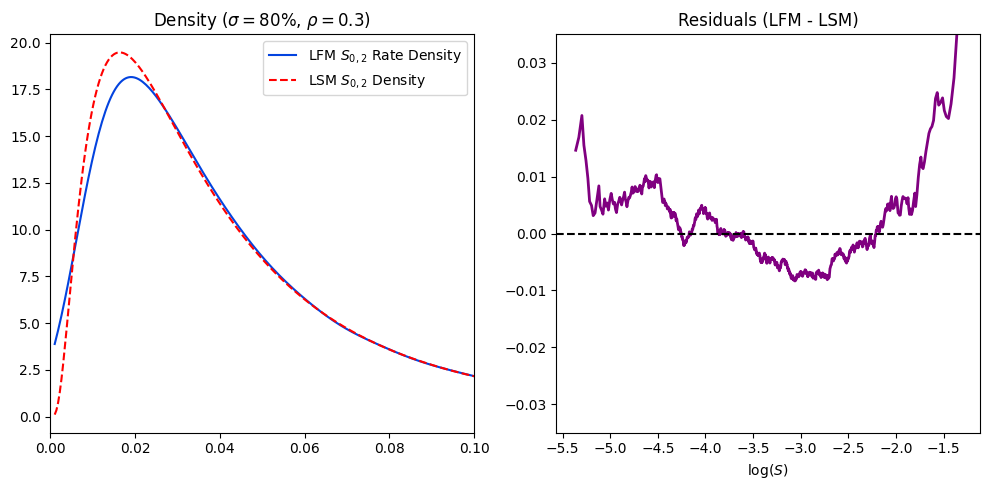
\includegraphics[width=0.48\linewidth]{images/swap_rate_0.8_0.3}\hfill
			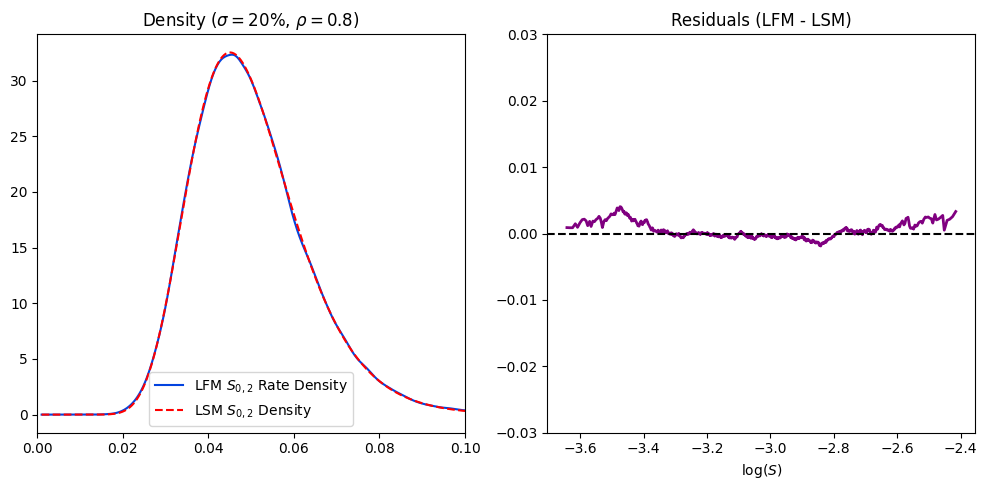
\includegraphics[width=0.48\linewidth]{images/swap_rate_0.2_0.8}
		\end{center}
	\end{itemize}
	\begin{tcolorbox}[colback=gray!5, colframe=maincolor, arc=0mm, boxrule=0.5pt]
		\footnotesize
		The discrepancy grows with: \textbf{high variance}: the log-normal distribution becomes increasingly skewed as volatility increases,
		\textbf{low correlation}: if $\rho = 1$, the sum behaves exactly like a single log-normal variable,	\textbf{long maturity}: Central Limit Theorem says that adding more variables, the sum moves toward a Normal distribution.
	\end{tcolorbox}
\end{frame}

\begin{frame}{Incompatibility between LFM and LSM}
	\begin{itemize}
		\item<1-> Consequently, it has been argued that, in normal market conditions, the two distributions are hardly distinguishable.
		\item<2-> Once ascertained the mathematical inconsistency of these two models, the problem left is choosing either of the two models for the whole market.
		\item<3-> After that choice, the half market consistent with the model is calibrated almost automatically, thanks to the corresponding Black’s formula, but the remaining half is a little more intricate to calibrate.
	\end{itemize}
\end{frame}

\begin{frame}{Proposed Solution}
	\begin{itemize}
		\item<1-> Although the LSM is particularly convenient when pricing a swaption, because it yields the practical Black’s formula for swaptions, for different products, even those involving the swap rate, there is no analytical formula in general.
		\item<2-> \textcolor{maincolor}{Also since the LIBOR forward rates, rather than swap rates, are more natural and representative coordinates of the yield curve usually considered}, besides being mathematically more manageable, the better choice of modeling may be to \textcolor{maincolor}{assume as framework the Log-normal Forward Libor Model}.
		\item<3-> Thus, hereafter, we are working under the hypothesis of the LFM.
		\item<4-> If we choose one of the discount bonds $P(\cdot, T_i)$ as a numeraire, one forward rate will be a martingale, however the swap rate, being a combination of several forward rates, will not.
		\item<5-> We thus conclude that \textcolor{maincolor}{swaption pricing via Black’s formula is not fully correct in the LFM}.
	\end{itemize}
\end{frame}

\begin{frame}{Proposed Solution}
	\begin{itemize}
		\item Brigo and Mercurio (2001) looked at the exact dynamics of the swap rate. Under the LFM, the swap rate follows a stochastic differential equation (SDE) where the drift and volatility terms are \textbf{incredibly messy} because they depend on the entire correlation structure of all underlying LIBOR rates.
		\begin{itemize}
			\item It involves complex integrals and state-dependent terms that make it nearly impossible to use for fast, real-time trading or "Greek" calculations.
		\end{itemize}
		\item Instead of using the exact SDE, they have developed Analytical Approximations (e.g. the Rebonato formula). These formulas "freeze" certain drift terms at their initial values ($t=0$), allowing you to map LFM volatilities to Swaption volatilities quite easily.
		\item Even if we can't find a pretty pencil-and-paper formula, swaptions under LFM can be easily evaluated with a Monte Carlo simulation.
	\end{itemize}
\end{frame}

\section{Monte Carlo Pricing}

\begin{frame}{Monte Carlo Pricing of Swaptions (LFM)}
	\begin{itemize}
		\item While Black-76 prices individual caplets/swaptions in \emph{isolation}, the LFM models the \textbf{joint dynamics} of the entire forward curve.
		\item You simulate the paths of all forward LIBOR rates $\{F_1, F_2, \ldots, F_n\}$ simultaneously, accounting for their correlations a.k.a.  their joint dynamics (SDEs) is discretized numerically.
		\item At the swaption expiry, you calculate the swap rate from those simulated LIBORs and check if it's "in the money."
		\item Unlike the approximations mentioned above, Monte Carlo doesn't care if the swap rate distribution is messy. It handles the complexity naturally. \textbf{The only downside is computational speed}.
		%		\item<1-> Brigo and Mercurio derived a complex expression for the swap rate dynamics under the $T$-forward measure induced by the numeraire $P(\cdot, T_i)$.
		%		\item<2-> But it is not much manageable. There exist, however, a very good approximate formulas to the swaption volatility which can be directly used to calibrate to a matrix of quoted swaption volatilities.
		%		\item<3-> Also, \textcolor{maincolor}{performing a Monte Carlo simulation to obtain the swaption price is anyway feasible.}
		
		%		\item It is the standard for path-dependent interest rate derivatives because it is calibrated directly to market-quoted volatilities.
		%		\item Rates $F_i(t)$ are modeled as diffusion processes. Because a swaption depends on a basket of these rates, we cannot price them independently; we must simulate the whole vector of rates simultaneously.
	\end{itemize}
\end{frame}

\begin{frame}{Monte Carlo Pricing of Swaptions (LFM)}
	\begin{itemize}
		\item First we need to decide which $T_i$ to use. A common (convenient) choice is to go with the \emph{Terminal Measure}, the one induced by the the bond maturing at the final tenor $P(t, T_\beta)$.
		\item The drift formula is significantly simpler and more computationally stable (note that only the final rate is a martingale).
		\item Recall the price of a payer swaption:
		\begin{equation*}
			\begin{aligned}
				\textbf{PSw} = \expect{Q}&\left[D(0, T_\alpha) (S_{\alpha,\beta}(T_\alpha) - K)^+ \sum_{i=\alpha+1}^\beta \tau_i P(T_\alpha, T_i)\right] \\
				&= P(0, T_i)\mathbb{E}^{T_i}\left[(S_{\alpha, \beta}(T_i) - K)^+ \sum^\beta_{i=\alpha+1} \tau_i P(T_i, T_{i+1})\right]
			\end{aligned}
		\end{equation*}
		by considering $P(\cdot, T_\beta)$ the numeraire.
	\end{itemize}
\end{frame}

\begin{frame}{Monte Carlo Pricing of Swaptions (LFM)}
	\begin{itemize}
		\item<1-> Keep in mind that $S_{\alpha,\beta}$ has an expression in terms of the relevant spanning forward rates, and notice that the expectation above depends on the joint distribution of the same $\bm{F}$’s.
		\item Under the Terminal Measure $P_N$, the dynamics for rate $F_i(t)$ are:
		\begin{equation*}
			\frac{dF_i(t)}{F_i(t)} =\sigma_i \sum_{k=1}^N C_{ik} dW_k(t) \underbrace{-\sum_{j=i+1}^{N-1} \frac{\delta_j F_j(t) \sigma_i \sigma_j \rho_{ij}}{1 + \delta_j F_j(t)}}_{\mu_i(t, F(t))}dt
		\end{equation*}
		\item The main component of the simulation are:
		\begin{itemize}
			\item $\sigma_i$: instantaneous volatility;
			\item $C$: Cholesky factor of the correlation matrix $\rho$ (if 2Y rate jumps, 3Y rate likely follows).
			\item drift $\mu_i$ is not constant; it changes as the rates $F_j$ evolve. To prevent arbitrage, we must adjust the drift of every rate that is not the numeraire (not martingale).
		\end{itemize}
		%		\item<2-> The dynamics of the $k$-th forward rate, for each $k = \alpha + 1,\ldots, \beta$, under $\mathbb{Q}^\alpha$ is (\cref{eq:forward_rat_dynamics_lfm})
		%		\begin{equation}
			%			dF_k(t) = \sigma_kF_k\sum_{j=\alpha+1}^k\frac{\rho_{kj}\tau_j\sigma_jF_j}{1+\tau_jF_j}dt+\sigma_kF_k dW^\alpha_k, \quad t<T_\alpha
			%			\label{eq:dynamics_4.1}
			%		\end{equation}
		%		and, in order to evaluate the swaption payoff we have to generate a number of realization of $F_{\alpha+1}(T_\alpha),\ldots, F_\beta(T_\alpha)$.
	\end{itemize}
\end{frame}

\begin{frame}{Algorithm Summary}
	The price of a payer swaption is estimated by simulating $m$ paths of the forward rates up to the option expiry $T_\alpha$.
	
	\begin{enumerate}
		\item Use an Euler scheme to update $F_i$ at each step $\Delta t$.
		\item For each path $j$, calculate the swap rate $S_{\alpha,\beta}^j$ and the annuity $A_{\alpha,\beta}^j$:
		\[ \Pi_j = (S_{\alpha,\beta}^j(T_\alpha) - K)^+ \sum_{i=\alpha+1}^\beta \tau_i P^j(T_\alpha, T_i) \]
		\item Finally you can estimate the swaption value as
		\begin{equation*}
			\mathbf{PSw} \approx \frac{P(0, T_\beta)}{m} \sum_{j=1}^m \frac{\Pi_j}{P^j(T_\alpha, T_\beta)}
		\end{equation*}
	\end{enumerate}
\end{frame}


\begin{frame}{Cholesky Decomposition \colablink{https://colab.research.google.com/drive/1p8aGbiX_tuetiuPx-lStR2EWDNZGCMrK}}
	\begin{itemize}
		\item Standard Monte Carlo generators produce \textbf{independent} random variables $Z \sim \mathcal{N}(0, I)$.
		\item But financial assets or physical variables are often \textbf{correlated}. We need a transformation matrix $C$ such that if we multiply it by independent "noise", the output has a specific covariance structure $\Sigma$.
	\end{itemize}
	
	\begin{block}{Definition}
		The Cholesky decomposition finds a lower triangular matrix $C$ such that:
		$$\Sigma = CC^T$$
		This $C$ acts as the "scaling factor" for correlation and results in
		\begin{equation*}
			C = \begin{bmatrix}
				1 & 0 \\
				\rho & \sqrt{1-\rho^2}
			\end{bmatrix}
		\end{equation*}.
	\end{block}
\end{frame}

\begin{frame}{LFM Calibration: From Market to Model}
	\begin{itemize}
		\item To get sensible results from our simulation we need to properly \textbf{calibrate} the LFM model, i.e. to find the set of parameters that best match the market values.
		\item In this particular case \emph{to calibrate} means to find $\sigma$ and $\rho$ such that the model recovers market prices of liquid instruments.
		\item When dealing with the pricing of swaptions under LFM the process is quite interesting and involves various steps:
	\end{itemize}
	\vfill
	\begin{enumerate}
		\item \textbf{Caplets} provide information about the \textbf{volatility} of individual forward rates;
		\item \textbf{Swaptions} provide information about the \textbf{correlation} between forward rates.
	\end{enumerate}
\end{frame}

\begin{frame}{LFM Calibration to Cap/Floor}
	\begin{itemize}
		\item Calibration of LFM to Cap/Floor is quite straightforward: you can derive the model volatilities $\sigma_i$ from the implied volatilities of cap, inverting the Black formula for cap from their market prices.
		\item The \textcolor{maincolor}{joint dynamics of forward rates is not involved in the pricing of a cap}, its payoff is just a sum of caplet payoffs, i.e. marginal distributions of forward rates are enough to compute the expectation, \textbf{correlation does not matter}.
		\item Indeed, there are no expectations involving two or more forward rates at the same time, so that correlations are not relevant.
	\end{itemize}
\end{frame}

\begin{frame}{Flat Volatilities}
	\begin{itemize}
		\item<1-> In the market, cap prices are \emph{not quoted in monetary terms}, but rather in terms \emph{of the implied Black volatilities}.
		\item<1-> When dealing with these contracts we need to distinguish two different kind of volatilities though.
		\item<2-> The implied \textcolor{blue}{flat volatilities} are the solutions ${\color{blue}v_{T_1-cap}},\ldots, \color{blue}{v_{T_n-cap}}$ of the equations
		\begin{equation*}
			\textbf{Cap}(t,\mathbf{F}, K) = \sum_{i=1}^j \textbf{Caplet}^{Bl}(t, F_i, K,{\color{blue}v_{T_j-cap}}),\quad j=1, \ldots,n
		\end{equation*}
		\item<3-> Although being quoted, \textcolor{maincolor}{flat volatilities have little financial meaning}.
		\item<3-> \textbf{Note} that the flat volatility $\color{blue}{v_{T_j-cap}}$ is that implied by the Black formula by putting the \textbf{same} average volatility in all caplets up to $T_j$.
	\end{itemize}
\end{frame}

\begin{frame}{Spot Volatilities}
	\begin{itemize}
		\item<1-> Conversely the \textcolor{green!50!black}{spot volatilities} cannot be observed directly but are the quantities \textcolor{maincolor}{naturally tied to forward rates as a measure of their uncertainty}.
		\item<1-> They are the solutions ${\color{green!50!black}v_{T_1-caplet}},\ldots, \color{green!50!black}{v_{T_n-caplet}}$ of
		\begin{equation*}
			\textbf{Caplet}(t,F_i,K) = \textbf{Caplet}^{Bl}(t, F_i, K,{\color{green!50!black}v_{T_i-caplet}}),\quad i=1, \ldots,n
		\end{equation*}
		so they are just the implied average volatility from a caplet over $[T_{i-1}, T_i]$.
		\item<2-> To recover correctly cap prices according to the LFM dynamics, we need to have
		\begin{equation}
			\textbf{Cap} = \sum_{i=1}^j\textbf{Caplet}^{Bl}(t,F_i, K,{\color{blue}v_{T_j-cap}}) = \sum_{i=1}^j\textbf{Caplet}^{Bl}(t,K,F_i,{\color{green!50!black}v_{T_i-caplet}})
			\label{eq:spot_flat_vola}
		\end{equation}
		\item<3-> Notice that since the same average volatility $\color{blue}{v_{T_{j-cap}}}$ is assumed for all caplets in the $T_j$-maturity cap, there is some inconsistency because the same caplet is linked to different volatilities when concurring to different caps.
	\end{itemize}
\end{frame}

\begin{frame}{Actual Calibration}
	The calibration procedure can be summarized as follows:
	\begin{enumerate}
		\item<1-> determine the implied volatilities of Cap/Floor by inverting the Black formula using the market quotes. Those are the ${\color{blue}v_{T_{j-cap}}}$ flat volatilities;
		\item<2-> recover the correct spot volatilities with a numerical procedure (i.e. \textbf{bootstrap}) from Eq.~\ref{eq:spot_flat_vola};
		\item<3-> finally we can go back to the instantaneous parameter of the model through
		\begin{equation}
			{\color{green!50!black}v_{T_{i-1}-caplet}^2} =\cfrac{1}{T_{i-1}} \int_0^{T_{i-1}}{\color{red}{\sigma^2_{i,j}}}dt %=\cfrac{1}{T_{i-1}}\sum_{j=1}^{i-1}\tau_{j-1,j}\sigma^2_{i,j}
		\end{equation}
		\textbf{Note} that different parametrizations of the instantaneous volatility $\sigma_{i,j}^2$ lead to different evolutions of its term-structures.
	\end{enumerate}
\end{frame}

\begin{frame}{Financial Bootstrapping}
	\begin{itemize}
		\item Bootstrapping is a widely used technique to derive financial quantities from others available in the market.
		\item The algorithm relies on a set of contracts (bonds, swaps, caps,\ldots) with different maturities from which, with an iterative procedure, the unknown variable can be extracted.
		\item As an example let's consider a set of coupon bearing bonds with annual frequency and with maturities ranging from 1 to 4Y. From the market we get their current quotes.
		\item Then we can solve the following system of equations:
		\begin{equation*}
			\begin{cases}
				\textbf{CB}_1(r_1) = P_1 \implies r_1 = \textbf{CB}_1^{-1}(P_1)\quad\text{(iter 1)}\\
				\textbf{CB}_2(r_1, r_2) = P_2 \implies r_2 = \textbf{CB}_2^{-1}(r_1, P_2)\quad\text{(iter 2)} \\
				\textbf{CB}_3(r_1, r_2, r_3) = P_3 \implies r_3 = \textbf{CB}_3^{-1}(r_1, r_2, P_3)\quad\text{(iter 3)} \\
				\textbf{CB}_4(r_1, r_2, r_3, r_4) = P_4 \ldots
			\end{cases}
		\end{equation*}
	\end{itemize}
\end{frame}

\begin{frame}{Caplet Volatility Bootstrapping \colablink{https://colab.research.google.com/drive/1rEtK3eFSZpvjDIBzHE_1PY1H-FBRr0Uv}}
	Let's \emph{strip} caplet volatilities from the following cap (\emph{flat}) volatilities (they referred to caps with 0.013 strike over EURIBOR-6M).
	\begin{columns}
		\column{0.5\linewidth}
		\begin{center}
			\begin{tabular}{|c|c|}
				\hline
				Maturity & Volatility \\
				\hline
				1y & 44\% \\
				\hline
				2y & 45\% \\
				\hline
				3y & 44\% \\
				\hline
				4y & 41\% \\
				\hline
				5y & 39\% \\
				\hline
			\end{tabular}
		\end{center}
		\column{0.5\linewidth}
		\begin{center}
			\begin{tabular}{|c|c|}
				\hline
				Pillar & Rate \\
				\hline
				3m & 0.0002 \\
				\hline
				6m & 0.0007 \\
				\hline
				12m & 0.0025 \\
				\hline
				2y & 0.0070 \\
				\hline
				3y & 0.0100 \\
				\hline
				5y & 0.0162 \\
				\hline
			\end{tabular}
		\end{center}
	\end{columns}
\end{frame}

\begin{frame}{Caplet Volatility Bootstrapping}
	\begin{enumerate}
		\item We start with the nearest instruments, i.e. the spot starting caplet with $6m$ maturity. For maturities shorter than the first quoted value we consider the volatility constant hence:
		\begin{equation*}
			\sigma^{spot}_{6m}= \sigma^{spot}_{6m,1y} = \color{green!50!black}{\sigma^{flat}_{1y}}
		\end{equation*}
		
		\item Let’s now price the $1y$ forward starting caplet with $6m$ maturity. Since market cap volatilities are quoted assuming \textbf{no-arbitrage} opportunities we can build the forward starting caplet as the difference of two caps:
		
		\begin{equation*}
			\begin{gathered}
				\textbf{Cpl}_{1y,1y6m}(\sigma^{spot}_{1y6m})=\textbf{Cap}_{1y6m}-\textbf{Cap}_{1y} \\[0.3cm]
				\textbf{Cap}_{1y6m}=\textbf{Cpl}_{6m}(\textcolor{red}{\sigma^{flat}_{1y6m}}) + \textbf{Cpl}_{6m,1y}(\textcolor{red}{\sigma^{flat}_{1y6m}}) + \textbf{Cpl}_{1y,1y6m}(\textcolor{red}{\sigma^{flat}_{1y6m}}) \\[0.3cm]
				\textbf{Cap}_{1y}=\textbf{Cpl}_{6m}(\textcolor{green!50!black}{\sigma^{flat}_{1y}}) + \textbf{Cpl}_{6m,1y}(\textcolor{green!50!black}{\sigma^{flat}_{1y}})
			\end{gathered}
		\end{equation*}
	\end{enumerate}
\end{frame}

\begin{frame}{Caplet Volatility Bootstrapping}
	\begin{columns}
		\column{0.5\linewidth}
		Unfortunately the $18m$ volatility is NOT quoted on the market, so we can:
		\begin{itemize}
			\item assume for the sake of simplicity that the volatility remains constant between $1y$ and $2y$ caps;
			\item use an interpolation method such as linear or cubic spline to get the $1y6m$ cap volatility.
		\end{itemize}
		\column{0.5\linewidth}
		\begin{center}
			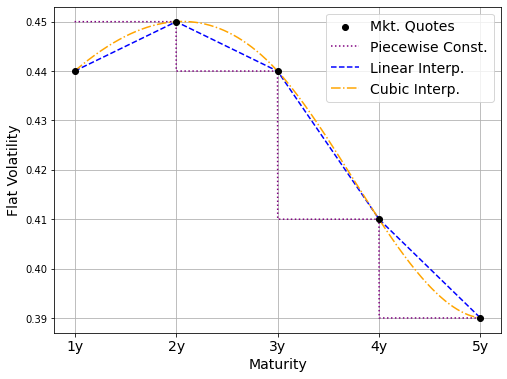
\includegraphics[width=0.8\linewidth]{images/flat_volatilities}
		\end{center}
	\end{columns}
	Once "estimated" $\sigma^{flat}_{1y6m}$ We will be able to solve a single volatility from previous Equation by using a Newton-Raphson or Brent methods.
\end{frame}

\begin{frame}{Caplet Volatility Bootstrapping}
	\begin{enumerate}
		\setcounter{enumi}{2}
		\item We can apply the same method for the $1y6m$ forward starting caplet to get the volatility, $\sigma^{flat}_{2y}$ is quoted so no interpolation is needed here.
		
		\begin{equation*}
			\begin{gathered}
				\textbf{Cpl}_{1y6m,2y}(\sigma^{spot}_{2y})=\textbf{Cap}_{2y}-\textbf{Cap}_{1y6m} \\[0.3cm]
				\textbf{Cap}_{2y}=\textbf{Cpl}_{6m}(\textcolor{green!50!black}{\sigma^{flat}_{2y}}) + \textbf{Cpl}_{6m,1y}(\textcolor{green!50!black}{\sigma^{flat}_{2y}}) + \ldots + \textbf{Cpl}_{1y6m,2y}(\textcolor{green!50!black}{\sigma^{flat}_{2y}}) \\[0.3cm]
				\textbf{Cap}_{1y6m}=\textbf{Cpl}_{6m}(\textcolor{green!50!black}{\sigma^{flat}_{1y6m}}) + \textbf{Cpl}_{6m,1y}(\textcolor{green!50!black}{\sigma^{flat}_{1y6m}}) + \textbf{Cpl}_{1y,1y6m}(\textcolor{green!50!black}{\sigma^{flat}_{1y6m}})
			\end{gathered}
		\end{equation*}
		
		\item Keep iteratively to solve for all the remaining volatilities using the very same technique.
	\end{enumerate}
\end{frame}

\begin{frame}[fragile]{Caplet Volatility Bootstrapping}
	\begin{center}
		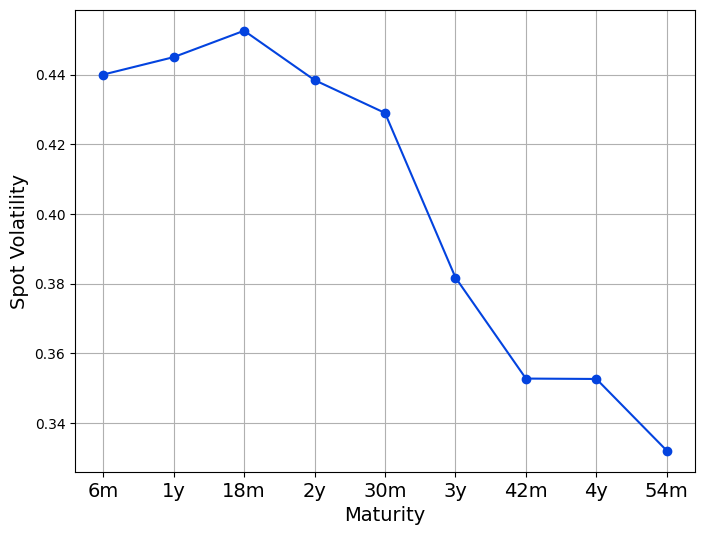
\includegraphics[width=0.65\linewidth]{images/spot_volatilities}
	\end{center}
\end{frame}

\begin{frame}{Instantaneous Volatility of Forward Rates}
	\begin{itemize}
		\item From \cref{eq:caplet_black_vol} ($v_i^2 = \frac{1}{T_{i-1}}\int_0^{T_{i-1}}\sigma_i^2(t)dt
		$) it is clear how it is impossible to uniquely determine the instantaneous volatility $\sigma_i(t)$ as there exist plenty of functions that would integrate to $v_i$.
		\item It is common to assume the $F_k$ has a \emph{piecewise-constant} volatility $\sigma_i(t)$ (constant in each maturity-expiry interval $i$).
		\item Nevertheless, to reduce the number of parameters of the model, further assumptions can be made (below some examples):
	\end{itemize}
	\begin{center}
		\begin{tabular}{|c|c|}
			\hline
			function of time-to-maturity & $\eta_{i-(\beta(t)-1)}$ \\ \hline
			constant regardless of $t$ & $s_i$ \\ \hline
			maturity/time to maturity & $\Phi_i\Psi_{i-(\beta(t)-1)}$ \\ \hline
			parametric & $[a(T_{i-1}-t) + d]e^{-b(T_{i-1}-t)} + c$ \\ \hline
		\end{tabular}
	\end{center}
\end{frame}

\begin{frame}{Remarks on LFM and Cap Pricing}
	\begin{itemize}
		\item In general, term structures of forward rate volatilities shape does not change significantly over time.
		\item Further, forward rate volatilites are low close to expiry, peak around 1-2 years and then fall off again (hump-shaped).
	\end{itemize}
	\begin{center}
		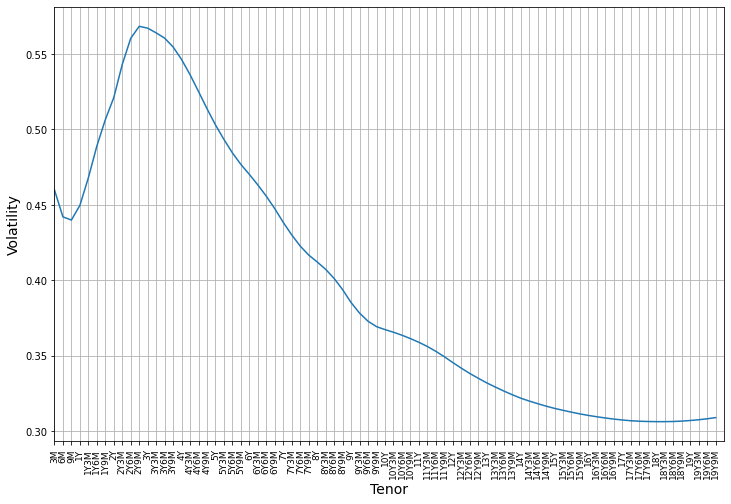
\includegraphics[width=0.5\linewidth]{images/cap_vola}
	\end{center}
\end{frame}

\begin{frame}{Remarks on LFM and Cap Pricing}
	\begin{itemize}
		\item A possible explanation of the humped shape is obtained by segmenting the caplet market across three maturities, (see Rebonato, 2002)
		\begin{enumerate}
			\item \textbf{Very short end of the curve}: central banks nowadays clearly communicate their strategy so that their actions are largely anticipated, leading to low volatilities in this region;
			\item \textbf{6M to 12-18M}: market participants continuously assess their expectations of future monetary policy, this is the region where subject beliefs have largest impact;
			\item \textbf{Longer maturities}: lastly, the third segment is much more affected by structural, long-term
			changes in expectations related to inflation and real rates/real returns. Thus, these long-term concerns are more or less independent of short-term monetary policies and the forward rate volatility is relatively low at the long end of the curve.
		\end{enumerate}
	\end{itemize}
\end{frame}

\begin{frame}{Functional Form for Instantaneous Volatility}
	One commonly used function is the parametric form specified in the previous table. This ensure a smooth term structure:
	\begin{equation*}
		\sigma_i(t) = [a(T_i - t) + b]e^{-c(T_i - t)} + d
	\end{equation*}
	\begin{columns}
		\column{0.5\linewidth}
		\begin{itemize}
			\item The parameters $\{a, b, c, d\}$ are calibrated to the entire Cap market simultaneously.
			\item This form captures the empirical reality that volatility often peaks for 1-2 year tenors before decaying (the hump).
			\item Finally it ensures that as time $t$ progresses in the Monte Carlo simulation, the volatility of the forward rates evolves realistically.
		\end{itemize}
		\column{0.5\linewidth}
		\begin{center}
			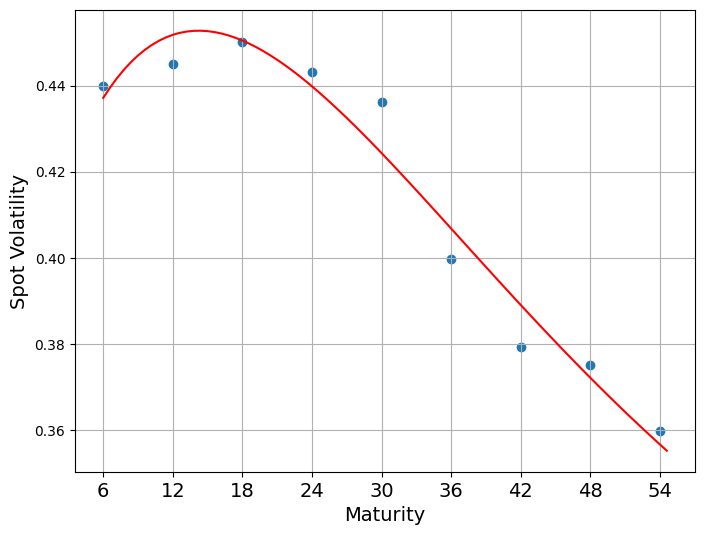
\includegraphics[width=0.8\linewidth]{images/caplet_spot_volatilities}
		\end{center}
	\end{columns}	
\end{frame}

\section{Correlated Brownian Motions}

\begin{frame}{Instantaneous vs. Terminal Correlation}
	\begin{itemize}
		\item<1-> Instantaneous Correlation ($\rho_{ij}$): summarizes the dependence between \textbf{changes} (shocks) of different forward rates at time $t$.
		\begin{equation*}
			\langle dW_i, dW_j \rangle = \rho_{ij} dt
		\end{equation*}
		\item<2-> Terminal Correlation: summarizes the dependence between the \textbf{levels} of two forward rates at a future time $T_i$.
		\item<3-> In the LFM, the terminal correlation is \textbf{not} solely determined by $\rho_{ij}$. It is heavily influenced by the \textit{path} of the instantaneous volatilities $\sigma_i(t)$.
	\end{itemize}
	\only<4-> {
		\begin{tcolorbox}[colback=gray!5, colframe=maincolor, arc=0mm, boxrule=0.5pt]
			\footnotesize
			While Caplets only care about the \textbf{average} volatility, Swaptions care about the \textbf{overlap} of volatility functions over time.
		\end{tcolorbox}
	}
\end{frame}

\begin{frame}{Terminal Correlation: An Example}
	Consider a payoff $\Pi = (\log F_3(T_1) - \log F_3(T_0))(F_2(T_1) - F_2(T_0))$ under the measure $\mathbb{Q}^2$:
	
	\begin{equation*}
		\begin{cases}
			dF_2(t) = \sigma_{2}(t)F_2(t)dW_2(t) \\
			dF_3(t) = \mu(t)dt + \sigma_{3}(t)F_3(t)dW_3(t)
		\end{cases}
	\end{equation*}
	
	\uncover<2->{
		The expectation $\mathbb{E}^2[\Pi]$ is a terminal-correlation dependent quantity:
		\begin{equation}
			\mathbb{E}^2[\Pi] = F_2(0)\rho_{2,3} \int_{0}^{T_1} \sigma_{2}(t)\sigma_{3}(t) dt
		\end{equation}
	}
	\uncover<3->{
		For a piecewise constant volatility ($\sigma_{k,1}$ on $[0, T_0]$ and $\sigma_{k,2}$ on $[T_0, T_1]$):
		\begin{equation*}
			\mathbb{E}^2[\Pi] = F_2(0)\rho_{2,3} \left( \sigma_{2,1}\sigma_{3,1}T_0 + \sigma_{2,2}\sigma_{3,2}(T_1 - T_0) \right)
		\end{equation*}
	}
\end{frame}

\begin{frame}{Derivation of the Expectation $\mathbb{E}^2[\Pi]$}
	\begin{itemize}
		\item \textbf{Step 1:} express increments as stochastic integrals:
		\[ \Delta F_2 \approx \int \sigma_2 F_2 dW_2, \quad \Delta \log F_3 \approx \int \sigma_3 dW_3 \]
		\item \textbf{Step 2:} use the property of \textbf{Stochastic Covariation}:
		\[ \mathbb{E}^2[\Delta \log F_3 \cdot \Delta F_2] =
		\mathbb{E}^2 \left[ \int \cdots dW_3 \cdot \int \cdots dW_2 \right] =
		\mathbb{E}^2 \left[ \int_{T_0}^{T_1} \sigma_2(t) F_2(t) \sigma_3(t) \rho_{2,3} dt \right] \]
		\item \textbf{Step 3:} Apply the Martingale property of $F_2$ under $\mathbb{Q}^2$:
		\[ \mathbb{E}^2[F_2(t)] = F_2(0) \]
		\item \textbf{Result:}
		\[ \mathbb{E}^2[\Pi] = F_2(0) \rho_{2,3} \int_{T_0}^{T_1} \sigma_2(t) \sigma_3(t) dt \]
	\end{itemize}
\end{frame}

\begin{frame}{Why Volatility Scheduling Matters}
	Assume $F_2(0)=F_3(0)=0.05$, $\rho_{2,3}=0.75$, and $\Delta T = 0.5$.
	Compare two cases that produce the \textbf{same Caplet prices} (same total variance):
	
	\vspace{0.4cm}
	\begin{center}
		\renewcommand{\arraystretch}{1.2}
		\begin{tabular}{lcccc}
			\toprule
			& \textbf{$\sigma_{2,1}$} & \textbf{$\sigma_{3,1}$} & \textbf{$\sigma_{2,2}$} & \textbf{$\sigma_{3,2}$} \\
			\midrule
			\textbf{Case A} & \textcolor{red}{0.50} & 0.10 & 0.10 & \textcolor{red}{0.50} \\
			\textbf{Case B} & 0.10 & 0.10 & \textcolor{blue}{0.50} & \textcolor{blue}{0.50} \\
			\bottomrule
		\end{tabular}
	\end{center}
	\vspace{0.4cm}
	
	\begin{itemize}
		\item \textbf{Case A (Low Overlap):} $F_2$ is volatile while $F_3$ is quiet. They don't "move together" in the same time bucket ($1.875\cdot 10^{-3}$).
		\item \textbf{Case B (High Overlap):} Both rates spike simultaneously in the second period. This creates much higher \textbf{joint covariance} ($4.875\cdot 10^{-3}$).
	\end{itemize}
	
	Even with the same correlation $\rho$, Case B will result in a \textbf{higher price} because the volatility "schedules" overlap (check the same exercise on Brigo-Mercurio pg. 235-236).
\end{frame}

\begin{frame}{Why Volatility Scheduling Matters}
	Check the same exercise on Brigo-Mercurio pg. 235-236.
	\begin{center}
		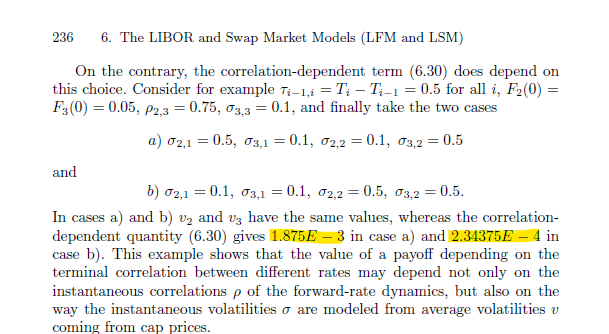
\includegraphics[width=0.8\linewidth]{images/brigo_mercurio_pg236}
	\end{center}
\end{frame}

\begin{frame}{Forward Rates Correlation}
	\begin{itemize}
		\item In order to calibrate $\rho$ we need to link the correlation to measurable quantity. It turns out that this link can be found with the swaption volatility.
		\item To compute it we need to express the variance of the swap rate $S_{\alpha,\beta}(t)$ in terms of the volatilities and correlations of the underlying forward rates $F_i(t)$.
		\item A swap rate for a period starting at $T_\alpha$ and ending at $T_\beta$ is defined as:
		\begin{equation*}
			S_{\alpha,\beta}(t) = \frac{P(t, T_\alpha)-P(t,T_\beta)}{\sum_{j=\alpha+1}^{\beta}\tau_jP(t,T_j)}
		\end{equation*}
		which is a non-linear function of multiple forward rates.
		\item To find how the volatility of the swap rate relates to the volatilities of the forward rates, we look at the change $dS$ (following Rebonato first order approximation)
		\begin{equation*}
			{dS} \approx \sum_{i=\alpha+1}^{\beta}\frac{\partial S}{\partial F_i}dF_i
		\end{equation*}
	\end{itemize}
\end{frame}

\begin{frame}{Rebonato Weights}
	\begin{itemize}
		\item To turn this into a relative change (which leads to volatility), we divide by $S$
		\begin{equation*}
			\frac{dS}{S} \approx \sum_{i=\alpha+1}^{\beta}\left(\frac{\partial S}{\partial F_i}\frac{F_i}{S}\right)\frac{dF_i}{F_i}
		\end{equation*}
		\item The term in the parentheses represents the elasticity ($w_i$) of the swap rate with respect to a specific forward rate.
		\item Rebonato’s idea has been to show that while $F_i$ and $S$ move over time, $\frac{\partial S}{\partial F_i}\frac{F_i}{S}$ stays constant (it can be considered \emph{frozen}).
	\end{itemize}
\end{frame}

\begin{frame}{Rebonato Weights}
	\begin{itemize}
		\item In practice, the most common analytical form for these weights is:
		\begin{equation*}
			w_i=\frac{\tau_i \prod_{j=n+1}^{i}\frac{1}{1+\tau_j F_j}}{\sum_{k=n+1}^{m}\tau_k\prod_{j=n+1}^{k}\frac{1}{1+\tau_jF_j}}
		\end{equation*}
		which can be derived considering that
		\begin{equation*}
			S(t) = \sum\frac{\tau_iP(t, T_i)}{A(t)}F_i(t)
		\end{equation*}
		\item This approximation is generally excellent for "at-the-money" (ATM) swaptions but can lose accuracy for deep out-of-the-money options where the skew becomes dominant.
	\end{itemize}
\end{frame}

\begin{frame}{The Connection}
	\begin{itemize}
		\item From the Taylor approximation we have seen before, we know:
		\begin{equation*}
			\frac{dS}{S} \approx \sum w_i \frac{dF_i}{F_i}
		\end{equation*}
		\item If we assume $dF_i/F_i=\sigma_i dW_i$, then the variance of the sum is the sum of the covariances:
		\begin{equation*}
			\text{Var}\left(\frac{dS}{S}\right) = \sum_i \sum_j w_i w_j \text{Cov} \left(\frac{dF_i}{F_i}\frac{dF_j}{F_j}\right) =
			\sum_{i=m}^{n-1} \sum_{j=m}^{n-1} w_i w_j \sigma_i \sigma_j \rho_{ij} \approx \sigma_{swaption}^2
		\end{equation*}
		where $\sigma_i$ have been determined from the caps, $w_i$ can be calculated with the Rebonato's formula and $\sigma_{swaption}$ can be read from the market.
		\item So solving for $\rho$ we can calibrate the forward rate correlation.
	\end{itemize}
\end{frame}

\begin{frame}{Parametric Correlation}
	\begin{itemize}
		\item Remember that $\rho$ is a $N\times N$ squared matrix with $N$ the number of forward rates modeled with LFM.
		\item To reduce the number of the model parameters, it is often assumed:
		\begin{equation*}
			\rho_{ij} = \exp(-\beta |T_i - T_j|)
		\end{equation*}
		where the coefficient $\beta$ has the opposite meaning of $\rho$\ldots
		\item If $\beta$ is high, rates are decoupled (low correlation).
		\item If $\beta = 0$, all rates move perfectly together.
		\item The calibration is performed by minimizing the error (distance between computed and market swaption volatilities) across a \textit{matrix} of swaptions with different maturities and tenors.
	\end{itemize}
\end{frame}

\begin{frame}{Two-Factor Correlation Model}
	\begin{itemize}
		\item The standard exponential decay $e^{-\beta \Delta T}$ often fails to capture long-term curve dynamics; a two-factor model can be then employed.
		\item We introduce a \textbf{Correlation Floor} $L$:
		\begin{equation*}
			\rho_{ij} = L + (1 - L)e^{-\beta |T_i - T_j|}
		\end{equation*}
		\item $L$ (Level): represents the "Parallel Shift". Even for rates very far apart, correlation never drops below $L$.
		\item $\beta$ (Decay): represents the "Twist." How quickly the curve decouples as tenors diverge.
	\end{itemize}
\end{frame}

\begin{frame}{Decorrelation}
	\begin{itemize}
		\item In the context of the Libor Forward Model (LFM) and the Two-Factor Correlation model we discussed, \textbf{decorrelation} refers to the phenomenon where forward rates of different tenors do not move perfectly in sync.
		\item If $\rho_{ij}=1$, rates are perfectly correlated. Decorrelation is the "slack" or "twist" in the curve.
		\item Recall the correlation structure: $\rho_{ij}=L+(1-L)e^{-\beta|T_i-T_j|}$, $\beta$ is the "decorrelation speed."
		\item If $\beta>0$, then as the distance between two tenors ($|T_i-T_j|$) increases, the correlation $\rho_{ij}$ drops.
		\item $L$ prevents "total decorrelation," ensuring that even the 1Y and 30Y rates maintain some fundamental connection.
	\end{itemize}
\end{frame}

\begin{frame}{Impact on Swaption Pricing}
	\begin{itemize}
		\item A Swaption is an option on a weighted basket of forward rates. Decorrelation is a primary driver of the basket's total volatility.
		\item If all rates are perfectly correlated, the volatility of the swap rate is simply the weighted average of the individual volatilities.
		\item If rates decorrelate, they can move in opposite directions. This "hedges" the basket, resulting in a lower swap rate volatility even if individual caplet volatilities remain high.
		\item By comparing the bootstrapped caplet volatilities to market swaption prices, you can "spot" whether the market is pricing in a high degree of decorrelation (a "twisting" curve) or low decorrelation (a "parallel" shifting curve).
	\end{itemize}
\end{frame}

\begin{frame}{Relation to the Terminal Measure Drift}
	\begin{itemize}
		\item Looking at the \textbf{drift} term in the Forward Rate SDE it is apparent how the decorrelation ($\rho_{ij}$) directly scales it.
		\item If rates are highly decorrelated (low $\rho_{ij}$), the "no-arbitrage" pull (the drift) exerted by the numeraire is weaker. If you assume perfect correlation when the market is actually decorrelated, your Monte Carlo simulation will overstate the drift, leading to biased prices.
		\item Decorrelation can be managed via PCA. The first component represents \emph{perfect correlation}, the second \emph{slope/twist} where one end of the curve goes up while the other goes down, the third \emph{curvature} further decorrelation of the belly of the curve relative to the wings.
		\item PCA reduces the original dimensions e.g. from $N\times N$ parameters in $\rho$ in the previous case you get $N\times N$ parameters only and the Euler scheme now needs three independent Brownian motions.
	\end{itemize}
\end{frame}

\begin{frame}{PCA on Term Structure \colablink{https://colab.research.google.com/drive/1DplGpcqLJRJp_xqeQPDfUFFnuuJtp3uX}}
	Historical data (2010-2025) tells how rates actually moved in the past. Can be used to determine the Correlation Matrix since it is generally stable.
	\begin{center}
		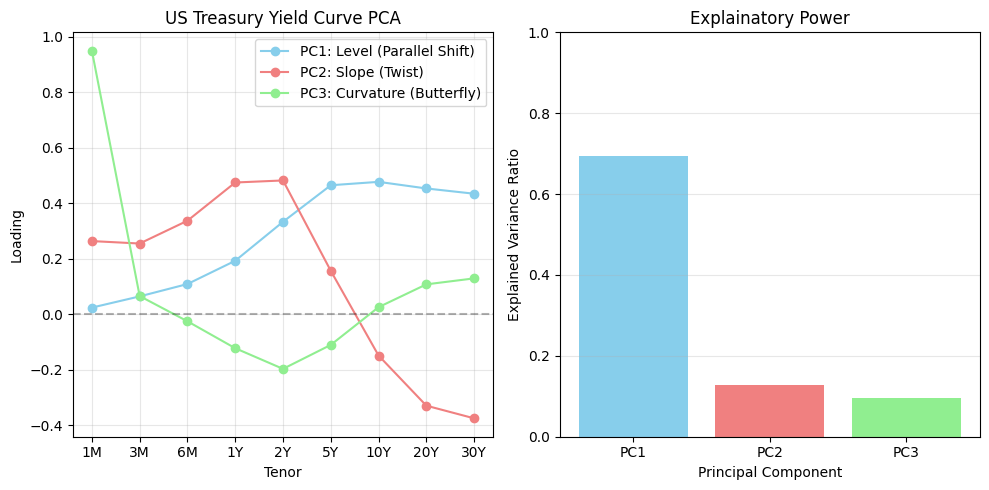
\includegraphics[width=0.65\linewidth]{images/pca_term_structure}
	\end{center}
	\begin{tcolorbox}[colback=gray!5, colframe=maincolor, arc=0mm, boxrule=0.5pt]
		\footnotesize
		PC1 the \emph{level} or parallel shift, explains about 70\% of the variance, PC2 the \emph{slope} or twist, explains 13\% of the variance, PC3 the \emph{curvature} or butterfly movement, explains another 9.6\% of the variance.
	\end{tcolorbox}	
\end{frame}

\subsection{Confidence Interval}
\begin{frame}{Confidence Interval}
	\begin{itemize}
		\item<1-> Consider a general payoff at time $T$, $\Pi(T)$, depending on a vector of spanning forward LIBOR rates $\bm{\tilde{F}}(t)$. %, for $t \in [0, T]$, where typically $T$ is smaller than or equal to the expiry of the first forward rate.
		\item<2-> We simulate various scenarios of $\Pi(T)$ under the $T$-forward measure. Let $m$ be the number of simulated paths, the Monte Carlo price of the payoff is
		\begin{equation*}
			\expect{Q}[D(0,T)\Pi(T)] = P(0,T)\mathbb{E}^T[\Pi(T)]\approx \frac{P(0,T)}{m}\sum_{j=1}^{m}\Pi_j(T)
		\end{equation*}
		\item<3-> Since $\Pi_1(T), \Pi_2(T),\ldots$ is a sequence of realizations of i.i.d. random variables distributed as $\Pi(T)$, the \textcolor{maincolor}{Central Limit Theorem} tell us that for $m\rightarrow\infty$
		\begin{equation*}
			\cfrac{\sum_{j=1}^{m}\Pi_j(T)-\mathbb{E}^T[\Pi(T)]}{\sqrt{m} \text{Std}(\Pi(T))}\rightarrow \mathcal{N}(0,1)
		\end{equation*}
	\end{itemize}
\end{frame}

\begin{frame}{Confidence Interval}
	\begin{columns}
		\column{0.6\linewidth}
		\begin{itemize}
			\item<1-> Thus, for large $m$, the following approximation holds
			\begin{equation*}
				\frac{\sum_{j=1}^{m}\Pi^j}{m}-\mathbb{E}^T[\Pi]\approx \frac{\text{Std}(\Pi)}{\sqrt{m}}\mathcal{N}(0,1)
			\end{equation*}
		\end{itemize}
		\column{0.4\linewidth}
		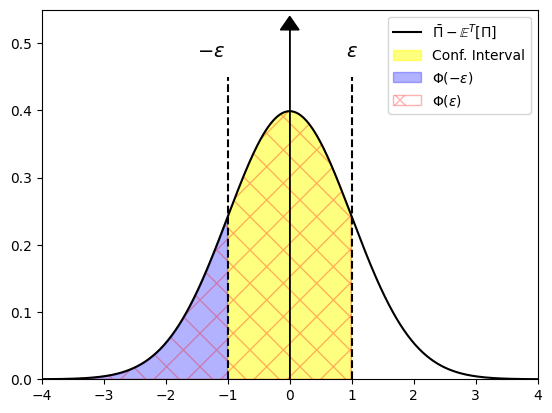
\includegraphics[width=0.9\linewidth]{images/epsilon}
	\end{columns}
	\begin{itemize}
		\item<2-> The probability that the MC estimate is closer than $\epsilon$ to the true price is
		\begin{equation*}
			P\left(\bigg|\frac{\sum_{j=1}^m\Pi_j}{m}-\mathbb{E}^T[\Pi]\bigg|<\epsilon\right) = P\left(|\mathcal{N}(0,1)|<\epsilon\frac{\sqrt{m}}{\text{Std}(\Pi)}\right) =
			2\Phi\left(\epsilon\frac{\sqrt{m}}{\text{Std}(\Pi)}\right)-1
		\end{equation*}
		where $\Phi$ denotes the CDF of the standard Gaussian distribution.
		\begin{equation*}
			P(|x|<\epsilon) = \Phi(\epsilon) - \Phi(-\epsilon) = \Phi(\epsilon) - (1 - \Phi(\epsilon)) = 2\Phi(\epsilon) - 1
		\end{equation*}
	\end{itemize}
\end{frame}

\subsection{Variance Reduction}
\begin{frame}{Monte Carlo Variance Reduction}
	To reduce the confidence interval without running too many simulations, i.e. reduce the sample variance, without increasing $m$, the \textcolor{maincolor}{control variate technique} can be used.
	\pause
	\begin{enumerate}
		\item<2-> Consider another payoff $\Pi_{an}$ which we can be evaluated analytically, whose expectation is denoted by $\mathbb{E}[\Pi_{an}] = \pi_{an}$, and simulate it together with $\Pi$ under the same scenarios.% for $\bar{F}$.
		\item<3-> Define an unbiased estimator for $\mathbb{E}[\Pi]$ as the sample mean of the random variable
		\begin{equation*}
			\Pi_c(\gamma) = \Pi + \gamma(\Pi_{an} - \pi_{an})
		\end{equation*}
		Hence $\Pi_c(\gamma)$ has expectation $\mathbb{E}[\Pi]$ and variance
		\begin{equation*}
			\text{Var}(\Pi_c(\gamma)) = \text{Var}(\Pi) + \gamma^2 \text{Var}(\Pi_{an}) + 2\gamma \text{Cov}(\Pi, \Pi_{an})
		\end{equation*}
	\end{enumerate}
\end{frame}

\begin{frame}{Monte Carlo Variance Reduction}
	\begin{enumerate}\addtocounter{enumi}{2}
		\item This can be minimized by choosing the appropriate $\gamma$ $\left(\text{from }\frac{\partial \text{Var}(\Pi_c)}{\partial\gamma}=0\right)$
		\begin{equation*}
			\gamma^* = -\frac{\text{Cov}(\Pi, \Pi_{an})}{\text{Var}(\Pi_{an})} = -\frac{\text{Corr}(\Pi, \Pi_{an})\text{Std}(\Pi)}{\text{Std}(\Pi_{an})}, \quad \left(\text{Corr}_{XY}=\frac{\text{Cov}_{XY}}{\text{Std}_X \text{Std}_Y}\right)
		\end{equation*}
		and the minimum variance of $\Pi_c$ is computed as
		\begin{equation*}
			\text{Var}(\Pi_c(\gamma^*)) = \text{Var}(\Pi)(1 - \text{Corr}(\Pi, \Pi_{an})^2)
		\end{equation*}
		that is \textcolor{maincolor}{smaller than the variance of $\Pi$}. Moreover, the \textcolor{maincolor}{larger the correlation between $\Pi$ and $\Pi_{an}$ the larger the difference between the two variances}.
	\end{enumerate}
\end{frame}

\begin{frame}{Monte Carlo Variance Reduction}
	\begin{enumerate}\addtocounter{enumi}{3}
		\item<1-> Moving to the standard deviation
		\begin{equation*}
			\text{Std}(\Pi_c(\gamma^*)) = \text{Std}(\Pi) \sqrt{1 - \text{Corr}(\Pi, \Pi_{an})^2}
		\end{equation*}
		the variance reduction will increase with the correlation between $\Pi$ and $\Pi_{an}$.
		\item<2-> Now if we consider the confidence interval for $\Pi_c$
		\begin{equation*}
			98\% C.L. =\left[\Pi_c(\gamma,m) - 2.33\cdot\frac{\text{Std}(\Pi_c)}{\sqrt{m}};\Pi_c(\gamma,m) + 2.33\cdot\frac{\text{Std}(\Pi_c)}{\sqrt{m}}\right]
		\end{equation*}
		we get a narrower width by a factor of
		\begin{equation*}
			\sqrt{1 - \text{Corr}(\Pi, \Pi_{an}; m)^2}
		\end{equation*}
	\end{enumerate}
	\only<3->{
		This technique is quite general and the \textcolor{maincolor}{choice of $\Pi_{an}$ is theoretically free}.
		In the case of the pricing of swaptions in the LFM, we select as $\Pi_{an}$ one of the simplest choice, the Black price of the swaption.
	}
\end{frame}

\begin{frame}{The "Black Formula" as Control Variate}
	\begin{itemize}
		\item While the LFM doesn't perfectly match the Black formula (due to the swap rate not being strictly log-normal), they are highly correlated ($>90\%$).
		\item We define the control variate based on the terminal payoff predicted by the Black model:
		\begin{equation*}
			\Pi_{an} = \frac{A_{\alpha,\beta}(T_\alpha)\cdot\textbf{Payoff}(S_{\alpha,\beta}(T_\alpha),K))}{P(T_\alpha, T_\beta)}
		\end{equation*}
		\item The current market price (today) of this "proxy" is known analytically
		\begin{equation*}
			\pi_{an}=PSw^{\text{Bl}}(0, S_{\alpha,\beta}, K, \sigma_{mkt})
		\end{equation*}
	\end{itemize}
\end{frame}

\begin{frame}{Implementation \& Efficiency}
	\begin{itemize}
		\item To reduce the width of the Confidence Interval, we construct the controlled estimator:
		\begin{equation*}
			\Pi_c(\gamma) = \Pi_{LFM} + \gamma(\Pi_{an} - \pi_{an})
		\end{equation*}
		\item Use the Black-76 formula with an approximate swap volatility (e.g., Rebonato’s formula) as $\pi_{an}$.
		\item To minimize variance, we set $\gamma^*=-\frac{\text{Cov}(\Pi_{LFM}, \Pi_{an})}{-\text{Var}(\Pi_{an})}$. %In practice, since they are so similar, $\gamma\approx -1$ is often used.
		\item The variance is reduced by $(1-\rho^2)$. Because the LFM swap rate is "nearly" log-normal, the correlation $\rho$ is nearly 1, making the Monte Carlo converge significantly faster.
	\end{itemize}
\end{frame}

\begin{frame}{LFM Swaption Pricing Summary \colablink{https://colab.research.google.com/drive/1mg-yoaZaKrhCQO7p0nzBnmV1X9Rfeuse}}
	\begin{enumerate}
		\item Bootstrap Cap volatilities to determine $v_{caplet}$;
		\item fit a parametric model for the volatilities to get $\sigma_i(t)$;
		\item compute Ribonato's weights and calibrate $\rho$ to the Swaption volatilities;
		\item reduce model parameters using a parametric expression for the correlation matrix;
		\item using Euler schema simulate LFM paths and compute the corresponding swap rate;
		\item improve MC efficiency using Control Variate with Swaption Black price;
		\item calculate the swaption payoffs and average to find the price estimate.
	\end{enumerate}
\end{frame}

\begin{frame}{LFM Simulation Checks (1/2)}
	A first set of checks can be done on swap rate expected properties.
	\begin{columns}
		\column{0.5\linewidth}
		\begin{center}
			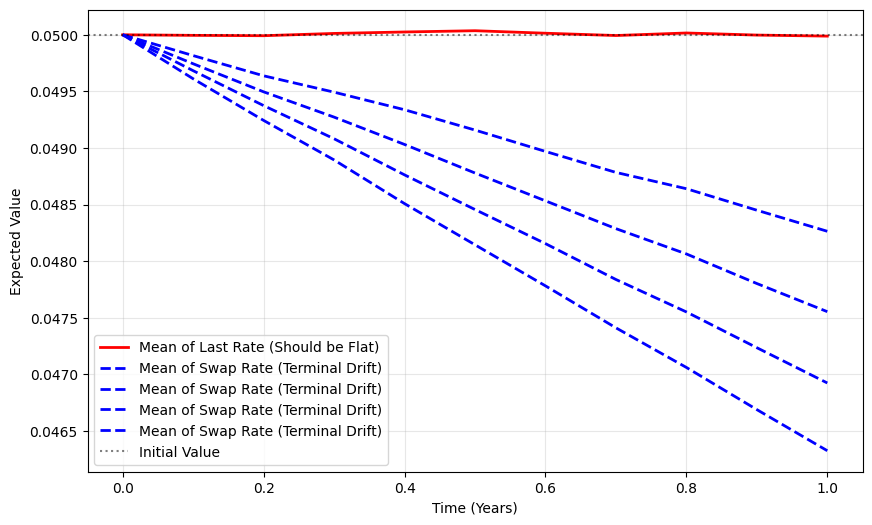
\includegraphics[width=0.85\linewidth]{images/lfm_martingale_check}
		\end{center}
		\begin{tcolorbox}[colback=gray!5, colframe=maincolor, arc=0mm, boxrule=0.5pt]
			\footnotesize
			In the Terminal Measure, the last rate $F_N$ must be a martingale, while the Swap Rate $S(t)$ will typically show a downward drift.
		\end{tcolorbox}	
		\column{0.5\linewidth}
		\begin{center}
			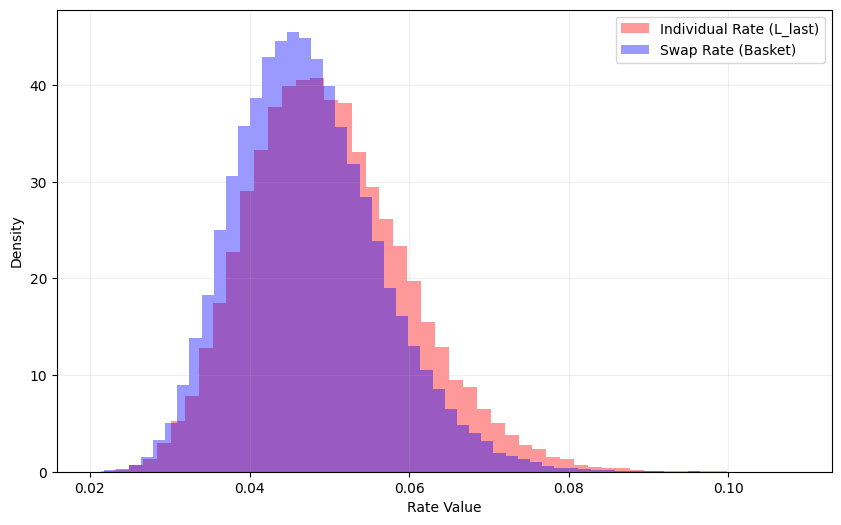
\includegraphics[width=0.85\linewidth]{images/lfm_log_normality_check}
		\end{center}
		\begin{tcolorbox}[colback=gray!5, colframe=maincolor, arc=0mm, boxrule=0.5pt]
			\footnotesize
			The comparison of a rate and the swap rate density should show a difference: the former is log-normal, the latter no.
		\end{tcolorbox}			
	\end{columns}
\end{frame}

\begin{frame}{LFM Simulation Checks (2/2)}
	A second set of checks can be devoted to the control variate technique.
	\begin{columns}
		\column{0.5\linewidth}
		\begin{center}
			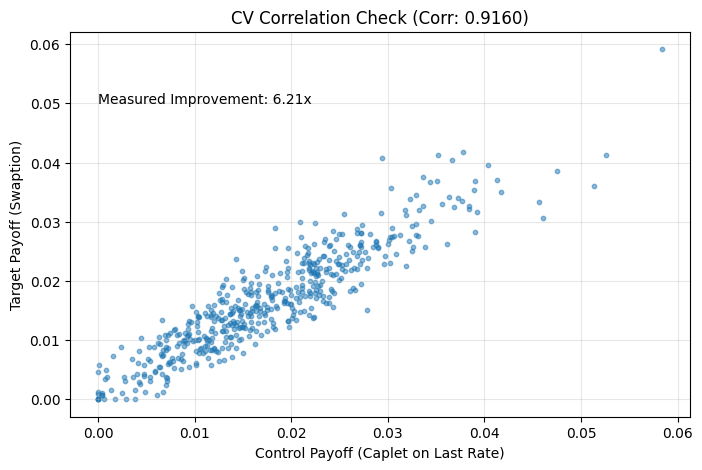
\includegraphics[width=0.85\linewidth]{images/lfm_correlation_check}
		\end{center}
		\begin{tcolorbox}[colback=gray!5, colframe=maincolor, arc=0mm, boxrule=0.5pt]
			\footnotesize
			Variance improvement is proportional to $k = \frac{1}{1-\rho^2}$. In our simulation $\rho = 0.916$ so $k\approx 6.2$.
		\end{tcolorbox}	
		\column{0.5\linewidth}
		\begin{center}
			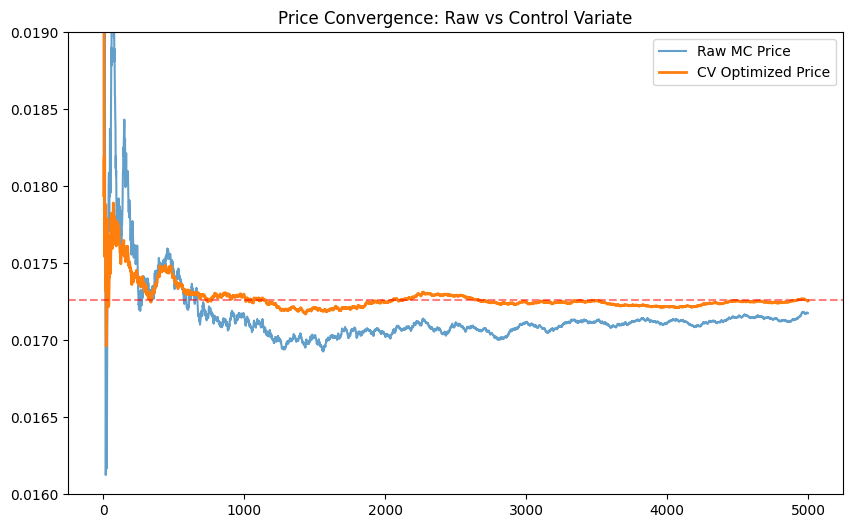
\includegraphics[width=0.85\linewidth]{images/lfm_convergence_check}
		\end{center}
		\begin{tcolorbox}[colback=gray!5, colframe=maincolor, arc=0mm, boxrule=0.5pt]
			\footnotesize
			The control variate MC should converge faster to the actual swaption price.
		\end{tcolorbox}			
	\end{columns}	
\end{frame}

\end{document}
